% ------------------------------------------------------------------------------
\subsection*{Exercise 4.2.1}

Figure \ref{fig:mp_421} illustrates the response of the minimum phase system
to step input changes and introduction of disturbances. Table \ref{tbl:mp_421}
summarizes some important performance metrics under this experiment.

\begin{figure}[H]\centering
  % This file was created by matlab2tikz.
%
%The latest updates can be retrieved from
%  http://www.mathworks.com/matlabcentral/fileexchange/22022-matlab2tikz-matlab2tikz
%where you can also make suggestions and rate matlab2tikz.
%
\definecolor{mycolor1}{rgb}{0.00000,0.44700,0.74100}%
\definecolor{mycolor2}{rgb}{0.85000,0.32500,0.09800}%
\definecolor{mycolor3}{rgb}{0.92900,0.69400,0.12500}%
\definecolor{mycolor4}{rgb}{0.49400,0.18400,0.55600}%
\definecolor{mycolor5}{rgb}{0.46600,0.67400,0.18800}%
%
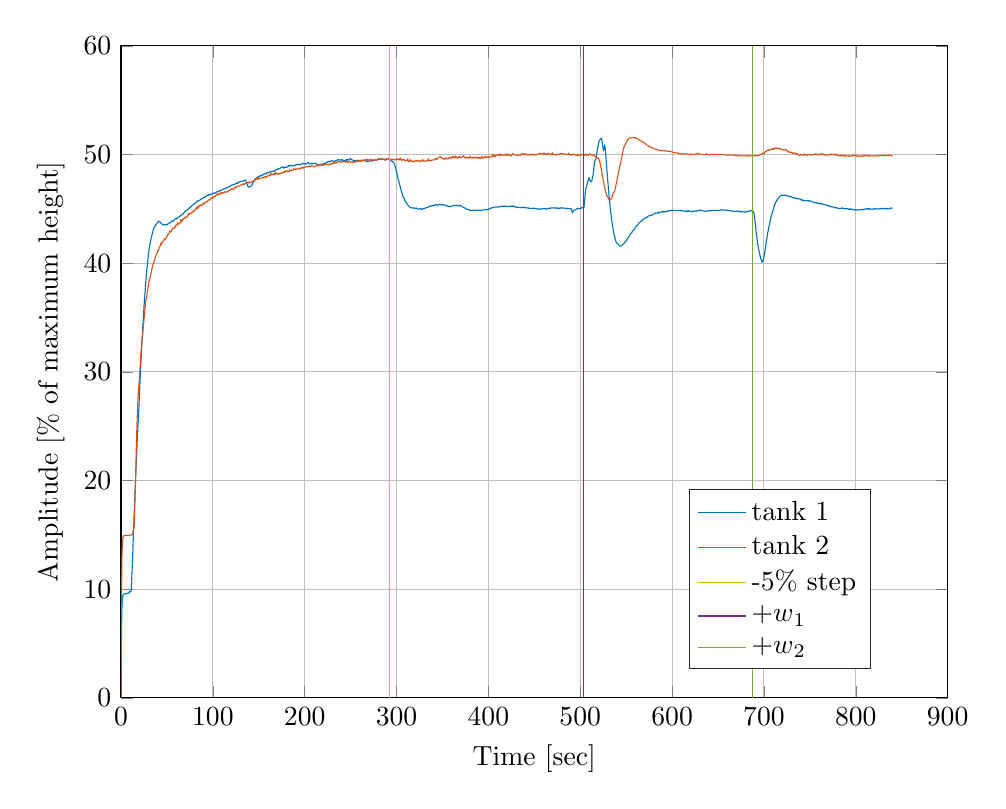
\begin{tikzpicture}

\begin{axis}[%
width=4.133in,
height=3.26in,
at={(0.693in,0.44in)},
scale only axis,
xmin=0,
xmax=900,
xlabel={Time [sec]},
xmajorgrids,
ymin=0,
ymax=60,
ylabel={Amplitude [$\%$ of maximum height]},
ymajorgrids,
axis background/.style={fill=white},
legend style={at={(0.687,0.044)},anchor=south west,legend cell align=left,align=left,draw=white!15!black}
]
\addplot [color=mycolor1,solid]
  table[row sep=crcr]{%
0	0\\
0.5	6.05648996035922\\
1	8.27496520165899\\
1.5	9.09141326001653\\
2	9.39373850655813\\
2.5	9.50319035988797\\
3	9.54271998908473\\
3.5	9.55567406789618\\
4	9.55699824870567\\
4.5	9.55931477514911\\
5	9.56777329017423\\
5.5	9.57999751748418\\
6	9.60899039734679\\
6.5	9.6240330140092\\
7	9.61232770196325\\
7.5	9.60328013367505\\
8	9.59094506325919\\
8.5	9.64673696195824\\
9	9.77553005657605\\
9.5	9.79964635400611\\
10	9.75602286264602\\
10.5	9.73215387778925\\
11	9.77855919164219\\
11.5	10.6796803553943\\
12	11.5925030910019\\
12.5	12.5985352442606\\
13	13.8354173155728\\
13.5	15.1224525875574\\
14	16.2814045483825\\
14.5	17.3717944671664\\
15	18.4212575587341\\
15.5	19.4571427850433\\
16	20.4886739640449\\
16.5	21.4376381632283\\
17	22.3981680058011\\
17.5	23.3589650895925\\
18	24.2199440692414\\
18.5	25.0347517586564\\
19	25.879778460284\\
19.5	26.8036323392352\\
20	27.8035813030334\\
20.5	28.7277776056845\\
21	29.6251537206489\\
21.5	30.5523284606727\\
22	31.4179095070416\\
22.5	32.2834706767403\\
23	33.084055637761\\
23.5	33.8249944853584\\
24	34.4998612414941\\
24.5	35.208646210549\\
25	35.9487454717547\\
25.5	36.567443451479\\
26	37.1446424403115\\
26.5	37.7676928027616\\
27	38.3591568755384\\
27.5	38.8450320285194\\
28	39.3083674345993\\
28.5	39.6993037910912\\
29	40.1340778400331\\
29.5	40.5525206801139\\
30	40.8880629024995\\
30.5	41.2133912965805\\
31	41.5196727125552\\
31.5	41.7651857383592\\
32	41.9941233708017\\
32.5	42.1741563691814\\
33	42.3512659655244\\
33.5	42.5199452839771\\
34	42.6788644620273\\
34.5	42.820236853883\\
35	43.0284524490621\\
35.5	43.18015359417\\
36	43.2698598001775\\
36.5	43.3401709415356\\
37	43.3927099908391\\
37.5	43.5096040136081\\
38	43.538507909481\\
38.5	43.6054404836658\\
39	43.6403442829823\\
39.5	43.7044392093669\\
40	43.7632444641656\\
40.5	43.8546067584914\\
41	43.8464810287199\\
41.5	43.8386465510536\\
42	43.7986974151758\\
42.5	43.7909124780781\\
43	43.7375137041423\\
43.5	43.6993329431254\\
44	43.6455381478744\\
44.5	43.6001677263587\\
45	43.5822834897525\\
45.5	43.566984919605\\
46	43.5313111053154\\
46.5	43.5416403336274\\
47	43.5586674928476\\
47.5	43.56505588797\\
48	43.5331604034799\\
48.5	43.5079067895594\\
49	43.5588569918585\\
49.5	43.525110044465\\
50	43.5335892220688\\
50.5	43.5644338699497\\
51	43.5964018361503\\
51.5	43.6456362082316\\
52	43.6652033723393\\
52.5	43.6905478760571\\
53	43.7282468999678\\
53.5	43.7386258397644\\
54	43.7631756010393\\
54.5	43.7815969275164\\
55	43.8702945439889\\
55.5	43.8599360773525\\
56	43.8724957828666\\
56.5	43.8802830938072\\
57	43.8618828049794\\
57.5	43.9214731848495\\
58	43.9908466503222\\
58.5	44.0228706614456\\
59	44.0639796528643\\
59.5	44.0846532433952\\
60	44.1195665714774\\
60.5	44.084168782271\\
61	44.0997640295739\\
61.5	44.1278305522506\\
62	44.1852914050014\\
62.5	44.2448397108019\\
63	44.2461395405653\\
63.5	44.2738871152909\\
64	44.3210661241488\\
64.5	44.3428660723137\\
65	44.3984971359819\\
65.5	44.4195230821752\\
66	44.4341188716654\\
66.5	44.4539187801774\\
67	44.4904008945571\\
67.5	44.5260450908966\\
68	44.5646969568448\\
68.5	44.6271618971908\\
69	44.6779689382947\\
69.5	44.7230992054857\\
70	44.7524775318636\\
70.5	44.8061740452256\\
71	44.844699351898\\
71.5	44.8603028384075\\
72	44.8893630129222\\
72.5	44.9484813923773\\
73	44.9724262061734\\
73.5	45.0036061771487\\
74	45.0213858434661\\
74.5	45.0841743181292\\
75	45.1327987887811\\
75.5	45.1455229840483\\
76	45.2058046948046\\
76.5	45.2253107807398\\
77	45.2605513394129\\
77.5	45.3124919002729\\
78	45.3348310730367\\
78.5	45.3806915715502\\
79	45.415114237437\\
79.5	45.460846896523\\
80	45.4706382079899\\
80.5	45.5388037639404\\
81	45.5409265639366\\
81.5	45.5853472758255\\
82	45.6080493926106\\
82.5	45.6541773420642\\
83	45.729671037972\\
83.5	45.7258886361353\\
84	45.7031153717253\\
84.5	45.7283435003738\\
85	45.7632236234671\\
85.5	45.7992889068998\\
86	45.8186063926102\\
86.5	45.8458127276863\\
87	45.9024402912497\\
87.5	45.8844178012695\\
88	45.9241491715061\\
88.5	45.9507004296008\\
89	45.9663682372009\\
89.5	45.9901833604842\\
90	46.0308712043831\\
90.5	46.0635335954851\\
91	46.0630890234275\\
91.5	46.0859470851161\\
92	46.0879791146156\\
92.5	46.1445779062804\\
93	46.1731449989387\\
93.5	46.2124282716135\\
94	46.259911531177\\
94.5	46.260885471609\\
95	46.2405429364195\\
95.5	46.290370287592\\
96	46.2904730582002\\
96.5	46.2880294879813\\
97	46.307281583696\\
97.5	46.3405630130023\\
98	46.3469046927393\\
98.5	46.3333283929033\\
99	46.3456102308556\\
99.5	46.3778456937301\\
100	46.4151436346193\\
100.5	46.4501836676011\\
101	46.4134768975807\\
101.5	46.4436568286815\\
102	46.4609174771516\\
102.5	46.4384420956924\\
103	46.492974096219\\
103.5	46.5161478978925\\
104	46.5380667805892\\
104.5	46.5767165258705\\
105	46.5610865108445\\
105.5	46.583282069026\\
106	46.5835505883255\\
106.5	46.6293321549721\\
107	46.6531290926095\\
107.5	46.632274216592\\
108	46.6912047245751\\
108.5	46.6753681800298\\
109	46.7036926757322\\
109.5	46.7288818492022\\
110	46.7656408693659\\
110.5	46.7734302579921\\
111	46.7835223558854\\
111.5	46.7965779429662\\
112	46.8282891124945\\
112.5	46.8436282539338\\
113	46.8430202312961\\
113.5	46.8604747286862\\
114	46.8861488663279\\
114.5	46.9243648680561\\
115	46.9670128901893\\
115.5	46.9719284988687\\
116	46.9827374815598\\
116.5	46.9754068941314\\
117	46.9954226958543\\
117.5	47.0031534193734\\
118	47.0498631361501\\
118.5	47.073357921183\\
119	47.0884994889779\\
119.5	47.135181694106\\
120	47.1770391207528\\
120.5	47.1613609032645\\
121	47.1725350640315\\
121.5	47.2007324865999\\
122	47.2240820791102\\
122.5	47.2480779080571\\
123	47.2506200817254\\
123.5	47.2516793398448\\
124	47.2820850239886\\
124.5	47.2954359934059\\
125	47.3027583254763\\
125.5	47.3198003297132\\
126	47.3941147255551\\
126.5	47.3472586438955\\
127	47.3544650115281\\
127.5	47.3798587944136\\
128	47.4371611404798\\
128.5	47.4493203950149\\
129	47.4866092786753\\
129.5	47.5163949160224\\
130	47.502500753781\\
130.5	47.5185514081343\\
131	47.5152550510035\\
131.5	47.5288455386484\\
132	47.5297014187604\\
132.5	47.5395812313484\\
133	47.5484332680582\\
133.5	47.5916249442752\\
134	47.60607054523\\
134.5	47.6155243702396\\
135	47.6529157137482\\
135.5	47.6299675801162\\
136	47.5524027286382\\
136.5	47.4376611149709\\
137	47.3202374577413\\
137.5	47.2004415512448\\
138	47.0907197937719\\
138.5	47.0315806699588\\
139	46.9983428254119\\
139.5	47.0134084097629\\
140	47.0355594419876\\
140.5	47.0456249580874\\
141	47.0653473346374\\
141.5	47.0908170976104\\
142	47.1317648384796\\
142.5	47.2016409562991\\
143	47.28568707249\\
143.5	47.367337185571\\
144	47.4509302799085\\
144.5	47.4958855790873\\
145	47.5747473505743\\
145.5	47.6576561007766\\
146	47.722174556831\\
146.5	47.7715040827569\\
147	47.8023208848885\\
147.5	47.8143886994259\\
148	47.867495263445\\
148.5	47.9132718634003\\
149	47.9303081732105\\
149.5	47.9485768886981\\
150	47.9677199839092\\
150.5	48.0050162233373\\
151	48.0084553921616\\
151.5	48.0335929781356\\
152	48.0403608266856\\
152.5	48.0819570500981\\
153	48.0848861220172\\
153.5	48.0417462960642\\
154	48.1023825907539\\
154.5	48.1389682903439\\
155	48.1321421234436\\
155.5	48.1735265037141\\
156	48.2275885400751\\
156.5	48.2168944480595\\
157	48.2214037303941\\
157.5	48.243424916674\\
158	48.2778163043274\\
158.5	48.2532955270738\\
159	48.3085751691793\\
159.5	48.2801525574489\\
160	48.2781021854048\\
160.5	48.3149587633933\\
161	48.3457226839872\\
161.5	48.3537823440687\\
162	48.3916538895877\\
162.5	48.3898178930458\\
163	48.4030498599323\\
163.5	48.4191328800562\\
164	48.4638828104738\\
164.5	48.4479433144995\\
165	48.4719357364311\\
165.5	48.4718941680474\\
166	48.4620769548832\\
166.5	48.4729379774751\\
167	48.4483909726292\\
167.5	48.4639308891879\\
168	48.5391927901733\\
168.5	48.5595096105072\\
169	48.5882107169439\\
169.5	48.6283148555518\\
170	48.6522766103857\\
170.5	48.6339524249146\\
171	48.6589352226761\\
171.5	48.6563865520607\\
172	48.6886347883209\\
172.5	48.6930100504318\\
173	48.7298903794382\\
173.5	48.7434414624618\\
174	48.7825991985674\\
174.5	48.8222822276557\\
175	48.8339942223745\\
175.5	48.8505575489304\\
176	48.7907001648176\\
176.5	48.770905097419\\
177	48.8178464350878\\
177.5	48.7626832721894\\
178	48.7854475856351\\
178.5	48.7988641404765\\
179	48.8448810052987\\
179.5	48.8154267988513\\
180	48.8134597649611\\
180.5	48.8118353887566\\
181	48.8581427771494\\
181.5	48.8924031589891\\
182	48.9035120072853\\
182.5	48.9701731876062\\
183	48.9513333126478\\
183.5	48.9403370800856\\
184	48.9756691924093\\
184.5	49.000736290941\\
185	48.9632577410309\\
185.5	48.9380131857206\\
186	48.9613328073419\\
186.5	48.9716500639442\\
187	48.9849563810944\\
187.5	48.9606049629947\\
188	48.9636238610329\\
188.5	48.9885985954222\\
189	48.9941230179204\\
189.5	49.0050270664154\\
190	49.0259800675891\\
190.5	49.0566545105091\\
191	49.0435175182975\\
191.5	49.0823217453664\\
192	49.0820490467779\\
192.5	49.056704198966\\
193	49.0780726552977\\
193.5	49.0765050232036\\
194	49.0540401288876\\
194.5	49.0444494591761\\
195	49.0530960927816\\
195.5	49.0635174570437\\
196	49.0651782086427\\
196.5	49.1134732759914\\
197	49.1221411343716\\
197.5	49.1572573019462\\
198	49.1940082578575\\
198.5	49.1527685065817\\
199	49.1434127213968\\
199.5	49.1291537129586\\
200	49.138973281758\\
200.5	49.1171472611454\\
201	49.1662250749989\\
201.5	49.1548316745862\\
202	49.1713324621916\\
202.5	49.2125686983631\\
203	49.2561237259927\\
203.5	49.2675745801298\\
204	49.2462937548808\\
204.5	49.1871566695126\\
205	49.166880672442\\
205.5	49.1359038464752\\
206	49.1659738588677\\
206.5	49.1606922130963\\
207	49.1324942691081\\
207.5	49.1329362901665\\
208	49.1488496133525\\
208.5	49.1530343286458\\
209	49.1378326620691\\
209.5	49.1451798932695\\
210	49.1748391415885\\
210.5	49.1779284149053\\
211	49.1752463700126\\
211.5	49.151674089913\\
212	49.1742529115418\\
212.5	49.1585327635677\\
213	49.1171311358253\\
213.5	49.0517963644007\\
214	49.0354460794176\\
214.5	49.0411887387587\\
215	49.0464792710607\\
215.5	49.0451889866814\\
216	49.0677862175393\\
216.5	49.0779729590547\\
217	49.091264006471\\
217.5	49.0426359184253\\
218	49.0970803471835\\
218.5	49.0629094175454\\
219	49.0770949698758\\
219.5	49.0904479000391\\
220	49.1333149099181\\
220.5	49.158815157662\\
221	49.1598060325066\\
221.5	49.2005621032811\\
222	49.1942686928579\\
222.5	49.1720924164025\\
223	49.2081024184738\\
223.5	49.2463548145821\\
224	49.2474380946035\\
224.5	49.3083616953051\\
225	49.3241918512617\\
225.5	49.3391757234278\\
226	49.3608980938548\\
226.5	49.3505977172369\\
227	49.349478315429\\
227.5	49.3604963070078\\
228	49.3325907217254\\
228.5	49.397521960182\\
229	49.4225144246033\\
229.5	49.4250987613711\\
230	49.3990199223884\\
230.5	49.394833982702\\
231	49.3683301378529\\
231.5	49.3363734272157\\
232	49.3687661100373\\
232.5	49.3809719325121\\
233	49.4038905524776\\
233.5	49.4504752848092\\
234	49.4524616126462\\
234.5	49.4616907384431\\
235	49.4775237735982\\
235.5	49.50301123172\\
236	49.4859047465191\\
236.5	49.5237847067005\\
237	49.5127610656761\\
237.5	49.5139169850399\\
238	49.4886989557894\\
238.5	49.4928847868928\\
239	49.4980652350817\\
239.5	49.5121114950453\\
240	49.5099411438827\\
240.5	49.4775900354986\\
241	49.5094935728028\\
241.5	49.4672066913846\\
242	49.4538312150432\\
242.5	49.426475777615\\
243	49.4319136537242\\
243.5	49.4417006852128\\
244	49.4477215143788\\
244.5	49.4778202707683\\
245	49.4846058314479\\
245.5	49.5238033877904\\
246	49.4659177181112\\
246.5	49.5181014199035\\
247	49.4943689517427\\
247.5	49.5294245729451\\
248	49.5452304546159\\
248.5	49.567944302183\\
249	49.592461783612\\
249.5	49.6113078250024\\
250	49.6105752011231\\
250.5	49.5460726601175\\
251	49.5490871577881\\
251.5	49.4789226028851\\
252	49.4792028713201\\
252.5	49.4748142965491\\
253	49.469877967526\\
253.5	49.4032634557576\\
254	49.3815240795817\\
254.5	49.4147135225147\\
255	49.3913281218661\\
255.5	49.43713172764\\
256	49.4207330392769\\
256.5	49.4219571636577\\
257	49.4431592086596\\
257.5	49.4231564610923\\
258	49.4471562340702\\
258.5	49.4630818271951\\
259	49.3937911336035\\
259.5	49.374974229459\\
260	49.4019686254999\\
260.5	49.3943477339273\\
261	49.403144773402\\
261.5	49.4040578219739\\
262	49.427012382677\\
262.5	49.439689165853\\
263	49.4375912251094\\
263.5	49.4334868916147\\
264	49.4577364708419\\
264.5	49.4692624023912\\
265	49.5009113746312\\
265.5	49.4829147510826\\
266	49.4941502026346\\
266.5	49.4443147179951\\
267	49.4077866766727\\
267.5	49.3734641810276\\
268	49.4021219340927\\
268.5	49.3693116088503\\
269	49.3269917665987\\
269.5	49.3748155835614\\
270	49.4056509983435\\
270.5	49.4194072056631\\
271	49.4088329003966\\
271.5	49.4194585753729\\
272	49.3986071869735\\
272.5	49.380949882133\\
273	49.3927502567072\\
273.5	49.4286424640005\\
274	49.4495604213425\\
274.5	49.4267434102216\\
275	49.4147209103409\\
275.5	49.4417070927315\\
276	49.4977053563626\\
276.5	49.4740548391446\\
277	49.4840099592172\\
277.5	49.4984221035098\\
278	49.5083207509431\\
278.5	49.495488494265\\
279	49.5229972935159\\
279.5	49.5467784052927\\
280	49.5801346424079\\
280.5	49.5636954760501\\
281	49.5743302402542\\
281.5	49.5816556079378\\
282	49.5520593874353\\
282.5	49.5554759230868\\
283	49.5823478135048\\
283.5	49.569976224796\\
284	49.5549500154589\\
284.5	49.6031491976606\\
285	49.560543980863\\
285.5	49.54961984422\\
286	49.5496170050566\\
286.5	49.5562273592521\\
287	49.5548175660826\\
287.5	49.5004836142512\\
288	49.5309251397488\\
288.5	49.5005067871668\\
289	49.5213720710214\\
289.5	49.5523372037312\\
290	49.5882609419837\\
290.5	49.584031707286\\
291	49.5666785629811\\
291.5	49.5836824207308\\
292	49.5442240888207\\
292.5	49.5075662893614\\
293	49.4466496895525\\
293.5	49.4346570964975\\
294	49.4107876203403\\
294.5	49.3966064056327\\
295	49.3656188186177\\
295.5	49.3452253610313\\
296	49.366565073089\\
296.5	49.3323045330627\\
297	49.2504563926321\\
297.5	49.1269421417695\\
298	49.0405697758976\\
298.5	48.898955187693\\
299	48.7404409769411\\
299.5	48.5653764829879\\
300	48.3610341458366\\
300.5	48.2142050675606\\
301	48.02712506016\\
301.5	47.8239996608017\\
302	47.6872391339362\\
302.5	47.5105136591953\\
303	47.3518314605574\\
303.5	47.1873466021359\\
304	47.0193654933265\\
304.5	46.8836977002652\\
305	46.740040658762\\
305.5	46.5495549322805\\
306	46.4294076670506\\
306.5	46.2241600317458\\
307	46.1299542801525\\
307.5	46.018459117547\\
308	45.9754422834087\\
308.5	45.9408295910208\\
309	45.7654858164252\\
309.5	45.7031001751752\\
310	45.6477490404436\\
310.5	45.5966288010733\\
311	45.5291207704213\\
311.5	45.443882446261\\
312	45.4000368083407\\
312.5	45.321991538602\\
313	45.2842651221903\\
313.5	45.2462303043153\\
314	45.2054493556829\\
314.5	45.1676349200052\\
315	45.1189164313693\\
315.5	45.1090332754924\\
316	45.1020077259385\\
316.5	45.0827895171134\\
317	45.0737802904847\\
317.5	45.0733920073759\\
318	45.0924190156117\\
318.5	45.0731424443257\\
319	45.0741299554903\\
319.5	45.0583653646703\\
320	45.0456772803023\\
320.5	45.0583596469517\\
321	45.0414815948342\\
321.5	45.0720645650069\\
322	45.0327571349295\\
322.5	45.0039580979395\\
323	44.9990067312025\\
323.5	44.9729327305861\\
324	44.977394530945\\
324.5	44.9774431721468\\
325	44.9779585581479\\
325.5	45.0029881052865\\
326	44.9886713690906\\
326.5	45.0327337084159\\
327	44.9858225599668\\
327.5	44.9369995208057\\
328	44.9666934578475\\
328.5	44.9816137840378\\
329	45.0298618533908\\
329.5	45.006102437743\\
330	45.0240835313939\\
330.5	45.0561044791282\\
331	45.0523044045697\\
331.5	45.0764892293499\\
332	45.0890488367452\\
332.5	45.0962654718701\\
333	45.1102127212131\\
333.5	45.1222804993146\\
334	45.1270323656678\\
334.5	45.1422042323367\\
335	45.15328454959\\
335.5	45.2033873679757\\
336	45.2360045172575\\
336.5	45.2594188168822\\
337	45.2696308674992\\
337.5	45.2408898194701\\
338	45.2351353794615\\
338.5	45.2571118262742\\
339	45.3013156430478\\
339.5	45.3117099687839\\
340	45.2890282422888\\
340.5	45.3174311023976\\
341	45.3098087468796\\
341.5	45.3288575176832\\
342	45.3371479058977\\
342.5	45.3887261435661\\
343	45.3830199870615\\
343.5	45.3667707678745\\
344	45.3587161330849\\
344.5	45.331940346544\\
345	45.3300669383779\\
345.5	45.3431293370974\\
346	45.3790257806515\\
346.5	45.4074018601937\\
347	45.3993990173593\\
347.5	45.3819063569748\\
348	45.3803092457667\\
348.5	45.3577099758489\\
349	45.3529715645996\\
349.5	45.3825714002703\\
350	45.3918837742845\\
350.5	45.3907796123151\\
351	45.366108789347\\
351.5	45.3501583195167\\
352	45.3576120426791\\
352.5	45.342864067412\\
353	45.2898360368705\\
353.5	45.2919136140518\\
354	45.2822717479204\\
354.5	45.2728952633274\\
355	45.2376131891012\\
355.5	45.254811981331\\
356	45.246839880605\\
356.5	45.2350114869687\\
357	45.2130224565916\\
357.5	45.1892765560238\\
358	45.2210606602207\\
358.5	45.218081826496\\
359	45.2190312543647\\
359.5	45.2453303417509\\
360	45.2491711710758\\
360.5	45.2599875888824\\
361	45.2917458308352\\
361.5	45.2972880641832\\
362	45.3166527098532\\
362.5	45.3004645406179\\
363	45.2927220363431\\
363.5	45.3106536659314\\
364	45.3154984443413\\
364.5	45.3199579982515\\
365	45.2943915792229\\
365.5	45.3279753533628\\
366	45.281971557783\\
366.5	45.2683154915273\\
367	45.2590123476355\\
367.5	45.2899714720021\\
368	45.3034716741844\\
368.5	45.2906221633884\\
369	45.3206560756932\\
369.5	45.2809688315294\\
370	45.279207484076\\
370.5	45.2521491240988\\
371	45.2502109880083\\
371.5	45.2232015601053\\
372	45.1762473196959\\
372.5	45.1412136747613\\
373	45.1164459068543\\
373.5	45.1070458455704\\
374	45.080880543568\\
374.5	45.071063662151\\
375	45.0355630508019\\
375.5	45.0071586600308\\
376	44.9742109766708\\
376.5	44.9655474115044\\
377	44.9518725274194\\
377.5	44.9420617350388\\
378	44.9259666586248\\
378.5	44.92250407416\\
379	44.9214356353743\\
379.5	44.8676211014634\\
380	44.8736893923697\\
380.5	44.8716602787808\\
381	44.8607608747359\\
381.5	44.8452372419456\\
382	44.851189031271\\
382.5	44.8428435089689\\
383	44.850345605149\\
383.5	44.8734749313914\\
384	44.8649643721515\\
384.5	44.8786332269673\\
385	44.8582113360847\\
385.5	44.8606532110635\\
386	44.8354485477535\\
386.5	44.8490648171278\\
387	44.8776604911869\\
387.5	44.8851025532322\\
388	44.8842721437833\\
388.5	44.863901361648\\
389	44.8643887888518\\
389.5	44.8473112651968\\
390	44.8392208327799\\
390.5	44.8617999096612\\
391	44.8688472043679\\
391.5	44.839136459829\\
392	44.8319053014284\\
392.5	44.8589279628672\\
393	44.8712058459305\\
393.5	44.8807883449332\\
394	44.8980641829053\\
394.5	44.8999928306767\\
395	44.8978355640898\\
395.5	44.9020495580427\\
396	44.8933485315507\\
396.5	44.9327788121348\\
397	44.9380044768807\\
397.5	44.9412475010665\\
398	44.9467824826101\\
398.5	44.904604670227\\
399	44.9438324705486\\
399.5	44.9547718470081\\
400	44.9681665072908\\
400.5	44.9589345639149\\
401	44.9910128278619\\
401.5	45.0083014076311\\
402	45.0272816547228\\
402.5	45.0413950517128\\
403	45.0771749149941\\
403.5	45.0701304627134\\
404	45.0876575151635\\
404.5	45.1182808496432\\
405	45.1169225802751\\
405.5	45.1173338390013\\
406	45.1236720250415\\
406.5	45.1502957986737\\
407	45.1564878761893\\
407.5	45.1554497112981\\
408	45.1707190554628\\
408.5	45.1754086173937\\
409	45.1501273492752\\
409.5	45.1578389814969\\
410	45.1546591605029\\
410.5	45.1569430762954\\
411	45.1738017205191\\
411.5	45.1886134626021\\
412	45.1695630046735\\
412.5	45.2147306581063\\
413	45.2382955488637\\
413.5	45.2329893931602\\
414	45.2279615645983\\
414.5	45.2247770013908\\
415	45.2227887240658\\
415.5	45.2439961395715\\
416	45.2305458646241\\
416.5	45.2549934427722\\
417	45.2363407398068\\
417.5	45.2224841703082\\
418	45.2309498943148\\
418.5	45.227181142372\\
419	45.2376836886724\\
419.5	45.2467830950952\\
420	45.2425029581668\\
420.5	45.2178436191239\\
421	45.1887676226989\\
421.5	45.1986118096427\\
422	45.2107978860563\\
422.5	45.2279138721185\\
423	45.218340151985\\
423.5	45.2320950189645\\
424	45.2549530513671\\
424.5	45.2567139222945\\
425	45.2340029347392\\
425.5	45.2387329262251\\
426	45.2364207367847\\
426.5	45.2560841372703\\
427	45.2041475574088\\
427.5	45.2332597452051\\
428	45.245344403977\\
428.5	45.2286958043711\\
429	45.1803276578267\\
429.5	45.1681639657607\\
430	45.1298076448154\\
430.5	45.1395235202414\\
431	45.1352009909979\\
431.5	45.1400107704704\\
432	45.1322673185969\\
432.5	45.1214323187958\\
433	45.1395931954385\\
433.5	45.134204791097\\
434	45.1382812244526\\
434.5	45.1304637562994\\
435	45.1262263259265\\
435.5	45.1088846690557\\
436	45.0938550134499\\
436.5	45.1310702893846\\
437	45.1305641260004\\
437.5	45.1435785547856\\
438	45.1353327140376\\
438.5	45.1480613790718\\
439	45.1059447724504\\
439.5	45.1216739692725\\
440	45.1119824393251\\
440.5	45.0965744019346\\
441	45.1000861856683\\
441.5	45.0954139907324\\
442	45.0846990918193\\
442.5	45.0777410235252\\
443	45.0602200273395\\
443.5	45.0823989282845\\
444	45.0607252794866\\
444.5	45.0450505385486\\
445	45.0126180208305\\
445.5	45.0297735763975\\
446	45.0495629337062\\
446.5	45.0349145125753\\
447	45.0319628946816\\
447.5	45.0404246994746\\
448	45.0499243036454\\
448.5	45.0620437596151\\
449	45.0408367957013\\
449.5	45.0394490009377\\
450	45.0523937634842\\
450.5	45.0272081652893\\
451	45.0204732045564\\
451.5	45.0307449380722\\
452	45.0293288260979\\
452.5	45.008546350654\\
453	44.9825856611204\\
453.5	44.9855553731982\\
454	44.9664971123583\\
454.5	44.9837406476317\\
455	44.9691082577025\\
455.5	44.9642567561863\\
456	44.9811899627829\\
456.5	44.9697268702088\\
457	44.9785687522915\\
457.5	44.9729086523263\\
458	45.001237626859\\
458.5	45.0172703049614\\
459	45.0368077451069\\
459.5	45.0097610620674\\
460	45.0244620155713\\
460.5	45.0275651865865\\
461	45.0198375020793\\
461.5	45.0298161076897\\
462	44.9905109663136\\
462.5	45.0105752986996\\
463	44.9752343976838\\
463.5	44.9896277304369\\
464	44.9964305262104\\
464.5	44.9920660986467\\
465	45.0400089009253\\
465.5	45.050549070041\\
466	45.0360991666124\\
466.5	45.0449251202505\\
467	45.0250433739639\\
467.5	45.0681670231166\\
468	45.0652345137335\\
468.5	45.0642888312848\\
469	45.0892906406128\\
469.5	45.0759209393537\\
470	45.0854998929149\\
470.5	45.0996219225681\\
471	45.067884390078\\
471.5	45.0887248585102\\
472	45.0768052833702\\
472.5	45.0633348718176\\
473	45.0741932344488\\
473.5	45.0735847348486\\
474	45.0765577736453\\
474.5	45.0502210668105\\
475	45.0613838579991\\
475.5	45.0903904425083\\
476	45.0223214765032\\
476.5	45.0219603457605\\
477	45.038761760339\\
477.5	45.0405355623648\\
478	45.059090688422\\
478.5	45.0664639786612\\
479	45.0821123280923\\
479.5	45.09176768918\\
480	45.0654175024347\\
480.5	45.0759841123406\\
481	45.0896188132931\\
481.5	45.0682426584674\\
482	45.0608531653565\\
482.5	45.0573479784743\\
483	45.0597276599081\\
483.5	45.0547248612461\\
484	45.0602458107854\\
484.5	45.0119893994665\\
485	45.0377744829597\\
485.5	45.0431151363946\\
486	45.0507014359991\\
486.5	45.0333793448575\\
487	45.0227737274557\\
487.5	45.0378545614634\\
488	45.0366652359212\\
488.5	45.0106457743129\\
489	44.9972523106587\\
489.5	45.004261538629\\
490	44.9635669450374\\
490.5	44.9798637169382\\
491	44.7852367277274\\
491.5	44.6650128206247\\
492	44.7063026947148\\
492.5	44.780740378885\\
493	44.8552673041516\\
493.5	44.887705027558\\
494	44.9010048080245\\
494.5	44.9057824320879\\
495	44.9105957352421\\
495.5	44.9439740224144\\
496	44.9756614053625\\
496.5	45.0083993603758\\
497	45.02954995677\\
497.5	45.0181808528049\\
498	45.0252181699175\\
498.5	45.0222221812323\\
499	44.997466539708\\
499.5	44.9984145325262\\
500	45.0053938511219\\
500.5	45.0568686991428\\
501	45.046958386952\\
501.5	45.0970577955208\\
502	45.098166579405\\
502.5	45.1177174558457\\
503	45.1244985821178\\
503.5	45.1289473977935\\
504	45.1026311705368\\
504.5	45.527641681859\\
505	45.9746511732828\\
505.5	46.4768778683657\\
506	46.7807526765792\\
506.5	46.9887902171606\\
507	47.0966277913026\\
507.5	47.2836714753737\\
508	47.444912256501\\
508.5	47.5721304589481\\
509	47.7325303802678\\
509.5	47.8310149538778\\
510	47.7734668001504\\
510.5	47.6256921100446\\
511	47.522057000809\\
511.5	47.4847586113586\\
512	47.512345308931\\
512.5	47.5676397622659\\
513	47.7057132443286\\
513.5	47.9445826002613\\
514	48.1094617719998\\
514.5	48.4808684920401\\
515	48.9619655972472\\
515.5	49.2964498974991\\
516	49.4528385112999\\
516.5	49.480387590756\\
517	49.550915141576\\
517.5	49.7160772572319\\
518	50.0802857474486\\
518.5	50.3692067769884\\
519	50.5410240742397\\
519.5	50.8217708754132\\
520	50.9953356183274\\
520.5	51.2278633821683\\
521	51.304574598064\\
521.5	51.3703436375169\\
522	51.4166067595155\\
522.5	51.4738890927902\\
523	51.469999903071\\
523.5	51.3578583947234\\
524	51.0760563480234\\
524.5	50.7202814371551\\
525	50.4574689023581\\
525.5	50.3924024401467\\
526	50.5431375381369\\
526.5	50.7913360892052\\
527	50.6760522507036\\
527.5	50.2740481885696\\
528	49.746271156132\\
528.5	49.1410740604767\\
529	48.5853392858267\\
529.5	48.0544653351997\\
530	47.5612002978665\\
530.5	47.0512379767323\\
531	46.563706897519\\
531.5	46.0911475502657\\
532	45.6482028680573\\
532.5	45.2162775927804\\
533	44.8148357305154\\
533.5	44.4693609454421\\
534	44.1318085097755\\
534.5	43.8090361437385\\
535	43.5359091900317\\
535.5	43.275189552203\\
536	43.0196677545113\\
536.5	42.7556889460667\\
537	42.6232475218357\\
537.5	42.4257518374312\\
538	42.2314411254756\\
538.5	42.0910149579364\\
539	41.9682105558353\\
539.5	41.8772762408515\\
540	41.8352794743761\\
540.5	41.8159387209298\\
541	41.7600471528342\\
541.5	41.7141505438521\\
542	41.6485542267397\\
542.5	41.6118169769829\\
543	41.5776227328356\\
543.5	41.5893896138354\\
544	41.5852084254278\\
544.5	41.582512846463\\
545	41.6183430112559\\
545.5	41.6668784005471\\
546	41.6768970866908\\
546.5	41.7191245792441\\
547	41.7623465296456\\
547.5	41.8159045345614\\
548	41.8485503056989\\
548.5	41.8903992403155\\
549	41.9483098198598\\
549.5	42.0105711170564\\
550	42.0385109216396\\
550.5	42.1096447405534\\
551	42.1923683092352\\
551.5	42.2440842962437\\
552	42.2975500320003\\
552.5	42.3766844448174\\
553	42.4514407487553\\
553.5	42.5168133521541\\
554	42.5806766289946\\
554.5	42.6742101032671\\
555	42.7094556707377\\
555.5	42.7467607823208\\
556	42.7759922846428\\
556.5	42.8901528525819\\
557	42.9455002047882\\
557.5	43.0093316131289\\
558	43.0494031254186\\
558.5	43.0823629864856\\
559	43.1542350976557\\
559.5	43.227477194793\\
560	43.3046799374533\\
560.5	43.354560059985\\
561	43.4181084920206\\
561.5	43.4260067830199\\
562	43.4589674543564\\
562.5	43.5109624186383\\
563	43.5909284394285\\
563.5	43.6426902576723\\
564	43.7218997797565\\
564.5	43.7326018651179\\
565	43.7626484472546\\
565.5	43.8028607346357\\
566	43.8231702966289\\
566.5	43.8932178834647\\
567	43.9216017217275\\
567.5	43.9532541677183\\
568	43.9945858083863\\
568.5	44.0546102899238\\
569	44.0607384172605\\
569.5	44.0890290980798\\
570	44.103463077174\\
570.5	44.1420931857731\\
571	44.1720696774335\\
571.5	44.1996610992854\\
572	44.2199982939869\\
572.5	44.2319661844244\\
573	44.2168898573423\\
573.5	44.268280461055\\
574	44.3261178728817\\
574.5	44.3449902107936\\
575	44.3501352752916\\
575.5	44.4006272709232\\
576	44.3872816116011\\
576.5	44.4140758654238\\
577	44.3891957005226\\
577.5	44.3885916110753\\
578	44.4026096429297\\
578.5	44.4547626133291\\
579	44.4695674627695\\
579.5	44.5064977602628\\
580	44.5106727963002\\
580.5	44.5411016342411\\
581	44.5574865634038\\
581.5	44.60711197491\\
582	44.6133399417842\\
582.5	44.6060215800182\\
583	44.6083881035042\\
583.5	44.6158928336134\\
584	44.6247557203283\\
584.5	44.6080377390324\\
585	44.6827916493338\\
585.5	44.6489441154742\\
586	44.6359338571704\\
586.5	44.6479732004424\\
587	44.6707533291089\\
587.5	44.6874392778296\\
588	44.7005952842658\\
588.5	44.720059435149\\
589	44.7520145003658\\
589.5	44.7124054236882\\
590	44.7094489316471\\
590.5	44.7563105415351\\
591	44.7087964450504\\
591.5	44.7269919067011\\
592	44.7110126733351\\
592.5	44.7251888203267\\
593	44.7561098378338\\
593.5	44.7241386163487\\
594	44.7611541603958\\
594.5	44.7562162100232\\
595	44.7694317799461\\
595.5	44.784797002716\\
596	44.8236221466891\\
596.5	44.8097372694359\\
597	44.8091200298324\\
597.5	44.8451265210137\\
598	44.82868345283\\
598.5	44.8302181969308\\
599	44.8557318879989\\
599.5	44.8529683561492\\
600	44.8302866849026\\
600.5	44.8525203301793\\
601	44.8634140602973\\
601.5	44.8497421825325\\
602	44.8679787361748\\
602.5	44.846829050653\\
603	44.844378179046\\
603.5	44.8528763938165\\
604	44.8473702233925\\
604.5	44.8507308775489\\
605	44.8575720685206\\
605.5	44.8547542586541\\
606	44.8427718622243\\
606.5	44.8367646252545\\
607	44.8622817577383\\
607.5	44.8619069622039\\
608	44.8273633499568\\
608.5	44.8233061408477\\
609	44.8285589350398\\
609.5	44.8209874508092\\
610	44.8262819538053\\
610.5	44.853678537738\\
611	44.8267322261536\\
611.5	44.8048701274781\\
612	44.8127762916523\\
612.5	44.8038302074895\\
613	44.780075932676\\
613.5	44.7787350016343\\
614	44.7630828173937\\
614.5	44.7927901801401\\
615	44.776971079916\\
615.5	44.8008542860866\\
616	44.7793627813093\\
616.5	44.7998073374811\\
617	44.7719960950341\\
617.5	44.803998867369\\
618	44.8342311933003\\
618.5	44.7845604474904\\
619	44.7644617964001\\
619.5	44.7577353702385\\
620	44.7703470875611\\
620.5	44.7607000839713\\
621	44.7522009557092\\
621.5	44.7368562046205\\
622	44.7458829123527\\
622.5	44.7793174889377\\
623	44.7635701777551\\
623.5	44.772263789223\\
624	44.7903469011864\\
624.5	44.7864676598879\\
625	44.7898523644611\\
625.5	44.7635186465185\\
626	44.793266011721\\
626.5	44.8130222344683\\
627	44.7966204058803\\
627.5	44.7899421612602\\
628	44.803679820862\\
628.5	44.8245014776579\\
629	44.8271200143922\\
629.5	44.8358999658239\\
630	44.8354961970772\\
630.5	44.8626379795121\\
631	44.882151244302\\
631.5	44.8284432922354\\
632	44.8301298031771\\
632.5	44.8144369803274\\
633	44.802673755979\\
633.5	44.8139068852056\\
634	44.8146019781534\\
634.5	44.8069407201516\\
635	44.7969280541507\\
635.5	44.7836248986234\\
636	44.7961849423873\\
636.5	44.7671605418299\\
637	44.7754487471017\\
637.5	44.7772161152582\\
638	44.7913225692971\\
638.5	44.7968098543629\\
639	44.8049463774959\\
639.5	44.8207114782064\\
640	44.8230223742794\\
640.5	44.8310045506446\\
641	44.8229552152465\\
641.5	44.8176971498209\\
642	44.8295737819442\\
642.5	44.8319165584452\\
643	44.8435512914517\\
643.5	44.8379063147381\\
644	44.8382331193307\\
644.5	44.8624119233784\\
645	44.8597127119371\\
645.5	44.8320943008745\\
646	44.8335156844391\\
646.5	44.8624400264526\\
647	44.8611979121574\\
647.5	44.8592324828691\\
648	44.8526034159334\\
648.5	44.8603033260879\\
649	44.8547387466399\\
649.5	44.8331565468159\\
650	44.8386093235791\\
650.5	44.8512111365687\\
651	44.8485193001356\\
651.5	44.8766235616546\\
652	44.8572834562634\\
652.5	44.8833472291366\\
653	44.8890521797406\\
653.5	44.9078554369266\\
654	44.8831294015791\\
654.5	44.9067341362845\\
655	44.9016672509283\\
655.5	44.8981118204084\\
656	44.8910247231321\\
656.5	44.8960568037245\\
657	44.8912088885082\\
657.5	44.8924093915531\\
658	44.900069559231\\
658.5	44.8923159582172\\
659	44.8698801106245\\
659.5	44.8847004981684\\
660	44.84892361432\\
660.5	44.8376661178056\\
661	44.8330540856734\\
661.5	44.8268586034856\\
662	44.8447579164069\\
662.5	44.8585296686552\\
663	44.8560676538966\\
663.5	44.8203593271541\\
664	44.7918591464795\\
664.5	44.8094335135522\\
665	44.7906518796317\\
665.5	44.7831610689625\\
666	44.7786362069856\\
666.5	44.7768000892949\\
667	44.7689269583516\\
667.5	44.7492555994716\\
668	44.74862088846\\
668.5	44.7443465631294\\
669	44.7559717986064\\
669.5	44.7505184708649\\
670	44.7785435085159\\
670.5	44.7807675228952\\
671	44.8151728697659\\
671.5	44.781736462099\\
672	44.7735249208421\\
672.5	44.7455236778678\\
673	44.7549064077304\\
673.5	44.7786034419449\\
674	44.7474663590657\\
674.5	44.7207854373238\\
675	44.7032620512981\\
675.5	44.7333032907555\\
676	44.7338520534017\\
676.5	44.7369732444982\\
677	44.7464177447468\\
677.5	44.7463419867693\\
678	44.7411049497819\\
678.5	44.7460717017595\\
679	44.7192442901367\\
679.5	44.694633598057\\
680	44.6852450457119\\
680.5	44.7132836494454\\
681	44.7338188150613\\
681.5	44.767546988675\\
682	44.770082310378\\
682.5	44.7343323727806\\
683	44.740773895396\\
683.5	44.7807740560057\\
684	44.7950174690206\\
684.5	44.7960157914281\\
685	44.8002113394178\\
685.5	44.8301996781779\\
686	44.823057367425\\
686.5	44.8156020210197\\
687	44.8338810823529\\
687.5	44.8028002686873\\
688	44.7915054728714\\
688.5	44.7216042751368\\
689	44.6304753072072\\
689.5	44.4218437383643\\
690	44.0805322766576\\
690.5	43.7091401057585\\
691	43.2943391578444\\
691.5	42.9013064303225\\
692	42.571247883816\\
692.5	42.2464488980339\\
693	41.962418824157\\
693.5	41.6696243204364\\
694	41.4026350906487\\
694.5	41.1868309503237\\
695	40.9893542470663\\
695.5	40.7810490770038\\
696	40.6142273502429\\
696.5	40.4436952993929\\
697	40.3447863670535\\
697.5	40.1934298074685\\
698	40.0944063521647\\
698.5	40.0914043051032\\
699	40.1868032586211\\
699.5	40.3630141582966\\
700	40.5654105434466\\
700.5	40.7868853353329\\
701	41.0374622430237\\
701.5	41.3296044008422\\
702	41.6246018229521\\
702.5	41.927011637183\\
703	42.2004803440903\\
703.5	42.4575432523942\\
704	42.7483167095557\\
704.5	42.9233984040477\\
705	43.138729409193\\
705.5	43.3846417152277\\
706	43.5560843447644\\
706.5	43.7662762221583\\
707	43.9571124226232\\
707.5	44.1704888326288\\
708	44.3406469095148\\
708.5	44.4628271827435\\
709	44.5996274206535\\
709.5	44.7437333709798\\
710	44.8800583928639\\
710.5	45.0151761713132\\
711	45.1784057645571\\
711.5	45.2981668979752\\
712	45.4418233958327\\
712.5	45.533835178229\\
713	45.6026603748648\\
713.5	45.703874695978\\
714	45.7843629113197\\
714.5	45.8326060014644\\
715	45.9114801802519\\
715.5	45.9453781116996\\
716	46.006298268773\\
716.5	46.0710393126035\\
717	46.1044399510964\\
717.5	46.1509447570867\\
718	46.1780718378918\\
718.5	46.2359684685584\\
719	46.223031552066\\
719.5	46.2456636467501\\
720	46.2331957441454\\
720.5	46.2594776861033\\
721	46.2629315121973\\
721.5	46.2361114523863\\
722	46.2502593515865\\
722.5	46.2421113033435\\
723	46.2264890531379\\
723.5	46.2490879495986\\
724	46.2312006882531\\
724.5	46.2371292486122\\
725	46.222172761496\\
725.5	46.1769801232109\\
726	46.1431603496219\\
726.5	46.1488803377606\\
727	46.1594479132776\\
727.5	46.1599748714903\\
728	46.1307591360547\\
728.5	46.1339818741639\\
729	46.1173591579152\\
729.5	46.1155189727091\\
730	46.0918531481924\\
730.5	46.0815551399481\\
731	46.0325092282355\\
731.5	46.05498290539\\
732	46.0342264309239\\
732.5	45.9986596008665\\
733	46.0099822055275\\
733.5	46.03439967383\\
734	45.9824951930459\\
734.5	45.9460204034527\\
735	45.9565468404087\\
735.5	45.9379494372695\\
736	45.9307216780879\\
736.5	45.9538401228439\\
737	45.9396532906144\\
737.5	45.9155135538639\\
738	45.9189578806488\\
738.5	45.92049272663\\
739	45.909798528551\\
739.5	45.8839240464267\\
740	45.8564069321878\\
740.5	45.8266657186797\\
741	45.7934684878164\\
741.5	45.831483836332\\
742	45.791582796316\\
742.5	45.7707083485639\\
743	45.7840623523434\\
743.5	45.7594707431144\\
744	45.7273952602438\\
744.5	45.7259501002747\\
745	45.7487262089718\\
745.5	45.7502330665309\\
746	45.7486377524778\\
746.5	45.7355118136598\\
747	45.7344240179984\\
747.5	45.7576943594971\\
748	45.7327828993589\\
748.5	45.7217157332085\\
749	45.7478780717753\\
749.5	45.747855101675\\
750	45.7200054504874\\
750.5	45.7085489110241\\
751	45.7169348084007\\
751.5	45.6710560098871\\
752	45.6486178861448\\
752.5	45.6357774772328\\
753	45.6375288584935\\
753.5	45.6104184304102\\
754	45.587812525935\\
754.5	45.5711783004524\\
755	45.5719458514157\\
755.5	45.574569311588\\
756	45.559588496423\\
756.5	45.5611324828963\\
757	45.5584036370598\\
757.5	45.5510018178835\\
758	45.5378010102966\\
758.5	45.4984718054264\\
759	45.487093806269\\
759.5	45.5042280072294\\
760	45.4751745009275\\
760.5	45.4629513651393\\
761	45.4792390798271\\
761.5	45.4651443244525\\
762	45.4908972272879\\
762.5	45.4836366867792\\
763	45.4685327276513\\
763.5	45.4320873564321\\
764	45.4081684445735\\
764.5	45.4098157086529\\
765	45.4108112246185\\
765.5	45.3925929899103\\
766	45.3830798941401\\
766.5	45.3949713303149\\
767	45.360393984161\\
767.5	45.3448093396832\\
768	45.3286688207954\\
768.5	45.2918582585957\\
769	45.2892127526828\\
769.5	45.3183082377863\\
770	45.280893755496\\
770.5	45.2549202442742\\
771	45.2567559322029\\
771.5	45.2541015401418\\
772	45.2126945109726\\
772.5	45.2145400258584\\
773	45.1874421173049\\
773.5	45.1893345132988\\
774	45.1912913729261\\
774.5	45.1795512921404\\
775	45.1659622007513\\
775.5	45.1545260589186\\
776	45.1508653206605\\
776.5	45.1285892192385\\
777	45.1087789562462\\
777.5	45.0892276787919\\
778	45.1013452767014\\
778.5	45.0926083618601\\
779	45.0938211360871\\
779.5	45.0845751619168\\
780	45.080291422778\\
780.5	45.0434140249997\\
781	45.0279861742511\\
781.5	45.0324867224792\\
782	45.0332933173263\\
782.5	45.0379033398487\\
783	45.012368135974\\
783.5	45.042296330137\\
784	45.0424741394818\\
784.5	45.0377285370935\\
785	45.0889663083465\\
785.5	45.0702398633686\\
786	45.0299822579157\\
786.5	45.0268315179075\\
787	45.0152461874009\\
787.5	45.0262577449601\\
788	45.0164141355463\\
788.5	44.9912869053215\\
789	45.0088302699114\\
789.5	45.0163059194015\\
790	45.0022023378661\\
790.5	45.0337057760483\\
791	45.0154448215445\\
791.5	44.9762778693604\\
792	44.9595559165182\\
792.5	44.9666203759819\\
793	44.9582376534781\\
793.5	45.0102343131418\\
794	44.9861196905355\\
794.5	44.9590667501608\\
795	44.9598141268719\\
795.5	44.9549915778702\\
796	44.9439998839935\\
796.5	44.9127304432314\\
797	44.9475042199566\\
797.5	44.9458692697176\\
798	44.899364874188\\
798.5	44.8982223536167\\
799	44.8901488754669\\
799.5	44.8962909379426\\
800	44.8836463791585\\
800.5	44.8919624840416\\
801	44.8848768611257\\
801.5	44.8961593786786\\
802	44.8871458329179\\
802.5	44.8827803964934\\
803	44.9026149930254\\
803.5	44.8950915100078\\
804	44.8947841144329\\
804.5	44.9211279561097\\
805	44.9309352440777\\
805.5	44.9081575260656\\
806	44.9184429075589\\
806.5	44.9274517234791\\
807	44.9276627109186\\
807.5	44.924858606623\\
808	44.9092706485569\\
808.5	44.9559638776901\\
809	44.9516538305227\\
809.5	44.9599224530901\\
810	44.9700212775382\\
810.5	44.9651639413193\\
811	45.0011668791721\\
811.5	45.00975150843\\
812	44.9899713372528\\
812.5	45.0181363974845\\
813	44.9870785130114\\
813.5	44.9997813082502\\
814	44.9685290531493\\
814.5	45.0192411772006\\
815	44.9690056597897\\
815.5	44.9791334617409\\
816	44.988535174689\\
816.5	44.9643008847868\\
817	44.9802844043565\\
817.5	44.9713625207043\\
818	44.9614091092722\\
818.5	44.9785221026368\\
819	44.9879421685088\\
819.5	44.9772993597362\\
820	44.9816269811624\\
820.5	45.0075343801886\\
821	44.9773485311058\\
821.5	44.9897379051637\\
822	45.0152016190803\\
822.5	44.9948262743383\\
823	44.999336055393\\
823.5	44.9881479352332\\
824	44.9904643274063\\
824.5	44.9920883979581\\
825	44.9874982114776\\
825.5	44.9736956545615\\
826	45.0029132906417\\
826.5	44.9930540107676\\
827	45.0144699430921\\
827.5	45.0426545132909\\
828	45.0249092364427\\
828.5	45.0227583351984\\
829	44.9978186363559\\
829.5	44.9949015569199\\
830	45.0339123429833\\
830.5	45.0202638265122\\
831	45.0275892356136\\
831.5	45.0407002957124\\
832	44.9991467075692\\
832.5	45.0073189681384\\
833	45.034429668091\\
833.5	45.015382945045\\
834	44.9910461223096\\
834.5	45.0232249882994\\
835	44.9813445511556\\
835.5	44.9973621706187\\
836	44.9872784930475\\
836.5	45.0290200007051\\
837	45.0245888084772\\
837.5	45.0316767780799\\
838	45.071573322048\\
838.5	45.0376466922561\\
839	45.0688618326781\\
839.5	45.0599650111225\\
840	45.0571319771424\\
};
\addlegendentry{tank 1};

\addplot [color=mycolor2,solid]
  table[row sep=crcr]{%
0	0\\
0.5	9.45409767787351\\
1	12.9313504344382\\
1.5	14.2104620353333\\
2	14.6793059155364\\
2.5	14.8521949801876\\
3	14.9161727057087\\
3.5	14.9378794167784\\
4	14.9474950257461\\
4.5	14.9510589025513\\
5	14.9501948758027\\
5.5	14.9511712940483\\
6	14.9508649827198\\
6.5	14.9477471827965\\
7	14.9457940170248\\
7.5	14.9448894754273\\
8	14.945883476838\\
8.5	14.9435668748379\\
9	14.9570011618668\\
9.5	14.9710111863529\\
10	14.9743988948455\\
10.5	14.975829107102\\
11	14.9818827837664\\
11.5	14.9851697436847\\
12	14.9873829366569\\
12.5	15.0060798169144\\
13	15.1783280801686\\
13.5	15.509096365028\\
14	15.5299977038011\\
14.5	16.260883316423\\
15	17.5479346813157\\
15.5	18.9579164883946\\
16	20.6027416574459\\
16.5	22.5532809247946\\
17	24.1340870474649\\
17.5	25.493798004952\\
18	26.5943822850828\\
18.5	27.6733602915395\\
19	28.2375150353567\\
19.5	28.7995921733243\\
20	29.422901510337\\
20.5	30.171864381369\\
21	30.7696258098397\\
21.5	31.4213259392402\\
22	32.0842013676181\\
22.5	32.4980116244946\\
23	32.9993403513618\\
23.5	33.4030248649374\\
24	33.892572917629\\
24.5	34.3512141730148\\
25	34.7687291675355\\
25.5	35.2005202181137\\
26	35.6166881003969\\
26.5	36.2586254237119\\
27	36.5972091416578\\
27.5	36.7018091898993\\
28	36.9224531370832\\
28.5	37.3580640949125\\
29	37.5144159497602\\
29.5	37.8037739192436\\
30	38.0935184596224\\
30.5	38.2984845143984\\
31	38.5307443190798\\
31.5	38.6190094725642\\
32	38.7754332178632\\
32.5	38.9589337916241\\
33	39.1949535431925\\
33.5	39.4773799841725\\
34	39.5366895914726\\
34.5	39.8082447461938\\
35	39.9345094114201\\
35.5	40.050864314703\\
36	40.1650379922726\\
36.5	40.320117031332\\
37	40.4026073417875\\
37.5	40.5378321018342\\
38	40.7066492038071\\
38.5	40.809428451767\\
39	40.8931972644294\\
39.5	40.9616578739819\\
40	41.1554892534377\\
40.5	41.1486432807726\\
41	41.2320171531962\\
41.5	41.3725610531842\\
42	41.4784049747976\\
42.5	41.5711665265975\\
43	41.7321453290878\\
43.5	41.8241249929877\\
44	41.7455703345359\\
44.5	41.8935138951656\\
45	41.9376904788739\\
45.5	41.9586103028005\\
46	41.9947737771412\\
46.5	42.0659515145191\\
47	42.2105390836613\\
47.5	42.2375852781536\\
48	42.198527314117\\
48.5	42.2581625869118\\
49	42.2736417002566\\
49.5	42.4016804441143\\
50	42.4444624284864\\
50.5	42.5183158264031\\
51	42.6470114507324\\
51.5	42.6280161118208\\
52	42.7103695121445\\
52.5	42.7820856165815\\
53	42.9325851109834\\
53.5	42.8802009976376\\
54	42.8633503447885\\
54.5	42.8733387087481\\
55	42.9957273356795\\
55.5	43.1245098968351\\
56	43.1940861917006\\
56.5	43.2237512676065\\
57	43.1918816868844\\
57.5	43.1836910745121\\
58	43.2316194904245\\
58.5	43.2834431935599\\
59	43.2933568770775\\
59.5	43.4619252141571\\
60	43.4441642962557\\
60.5	43.517282508511\\
61	43.5596980044544\\
61.5	43.6891967234287\\
62	43.6516367542411\\
62.5	43.5768336854981\\
63	43.6020534235331\\
63.5	43.6344757566744\\
64	43.6693893313469\\
64.5	43.7838068341958\\
65	43.9808835936122\\
65.5	43.9528752079304\\
66	43.8354447944845\\
66.5	43.9696140504714\\
67	44.0396088932421\\
67.5	44.0011232265833\\
68	44.0453062321717\\
68.5	44.1025321193921\\
69	44.145983720231\\
69.5	44.2033390426415\\
70	44.1562220975709\\
70.5	44.216419270255\\
71	44.2576403681004\\
71.5	44.2388635083922\\
72	44.2621655127703\\
72.5	44.3287567899106\\
73	44.5006243644275\\
73.5	44.5153279572195\\
74	44.469444628919\\
74.5	44.5852626051241\\
75	44.5491199218254\\
75.5	44.5294680653925\\
76	44.5363447563023\\
76.5	44.6569680588542\\
77	44.6420953312867\\
77.5	44.6654733352032\\
78	44.7358586034262\\
78.5	44.7299041223109\\
79	44.8451270512782\\
79.5	44.8638087608607\\
80	44.8162972488582\\
80.5	44.8675054843439\\
81	44.9110376529808\\
81.5	44.9509033723926\\
82	45.0975087346766\\
82.5	45.0084603914888\\
83	45.0463685273722\\
83.5	45.1275953159116\\
84	45.2202031716462\\
84.5	45.150605466263\\
85	45.233233618824\\
85.5	45.2598942543992\\
86	45.3565344207241\\
86.5	45.3574782835204\\
87	45.3107079785624\\
87.5	45.2855900245869\\
88	45.3328169336237\\
88.5	45.3777737335519\\
89	45.4189326504733\\
89.5	45.515120879925\\
90	45.4500574050621\\
90.5	45.4906771438118\\
91	45.5340669980928\\
91.5	45.5480317888775\\
92	45.5416912133329\\
92.5	45.6141386150486\\
93	45.645278500929\\
93.5	45.6342223002075\\
94	45.6836480551006\\
94.5	45.7226590680531\\
95	45.7770478757534\\
95.5	45.8106165918868\\
96	45.8442137678647\\
96.5	45.8376568886837\\
97	45.8156617894819\\
97.5	45.952870224178\\
98	45.9798679530169\\
98.5	45.9808785285981\\
99	46.004335483896\\
99.5	45.9663304360631\\
100	45.9581519124667\\
100.5	46.0488413239165\\
101	46.1031910181348\\
101.5	46.1052410704667\\
102	46.1255136036198\\
102.5	46.1416977662099\\
103	46.2126760430899\\
103.5	46.2315127688496\\
104	46.2615162338733\\
104.5	46.3770811719001\\
105	46.2920527053102\\
105.5	46.2796501736575\\
106	46.3354319558815\\
106.5	46.3909464358284\\
107	46.3680960282739\\
107.5	46.4267462054783\\
108	46.3891790724604\\
108.5	46.4197360240667\\
109	46.4739570828595\\
109.5	46.4907416673769\\
110	46.4273219152112\\
110.5	46.4350734815511\\
111	46.4864307678759\\
111.5	46.4719543099372\\
112	46.5008465330354\\
112.5	46.560721223393\\
113	46.5190263165701\\
113.5	46.5457860132199\\
114	46.5458508043281\\
114.5	46.5266551376002\\
115	46.5257675302082\\
115.5	46.5762006815786\\
116	46.5725558880713\\
116.5	46.5904703776344\\
117	46.6273232147859\\
117.5	46.678595457476\\
118	46.680616190579\\
118.5	46.6681866115734\\
119	46.7858892405982\\
119.5	46.8022243546699\\
120	46.7968649364609\\
120.5	46.8386395205335\\
121	46.830508223986\\
121.5	46.8083172631037\\
122	46.7660646874565\\
122.5	46.7732605156085\\
123	46.8711999132752\\
123.5	46.9549595253092\\
124	46.9328053879917\\
124.5	46.9437162440556\\
125	47.0096568954053\\
125.5	46.9882323302664\\
126	47.0266378033788\\
126.5	47.0350000568443\\
127	47.0699291337936\\
127.5	47.0949660589238\\
128	47.127314555339\\
128.5	47.1104674188488\\
129	47.1154974760719\\
129.5	47.1030018273816\\
130	47.1459103789008\\
130.5	47.1812540150626\\
131	47.2285337907265\\
131.5	47.2419835960378\\
132	47.2378844376173\\
132.5	47.2787730776627\\
133	47.2880755062926\\
133.5	47.2810836131467\\
134	47.242315101303\\
134.5	47.2490858898355\\
135	47.3263871258765\\
135.5	47.3270794365234\\
136	47.3516671599982\\
136.5	47.3797864964067\\
137	47.4167793404584\\
137.5	47.3991050342672\\
138	47.4243227624692\\
138.5	47.4357218463403\\
139	47.3942176999469\\
139.5	47.3996673470326\\
140	47.4523503907925\\
140.5	47.4220951032652\\
141	47.4139564268623\\
141.5	47.4152814427288\\
142	47.5132967316754\\
142.5	47.5328046374981\\
143	47.5183415927836\\
143.5	47.5103781570636\\
144	47.5554697866553\\
144.5	47.5974378102233\\
145	47.5865340050297\\
145.5	47.6042188311817\\
146	47.620161582743\\
146.5	47.6490301847384\\
147	47.7581039711336\\
147.5	47.8002265772265\\
148	47.7585829437595\\
148.5	47.7136388298611\\
149	47.7673346243119\\
149.5	47.7521420969029\\
150	47.8605671052432\\
150.5	47.8162989946809\\
151	47.7736654061233\\
151.5	47.8250382874648\\
152	47.8294268725757\\
152.5	47.8219781591392\\
153	47.8424831156892\\
153.5	47.8503167171078\\
154	47.8777546406586\\
154.5	47.8930088398914\\
155	47.8394927080102\\
155.5	47.8444426781011\\
156	47.9360629251175\\
156.5	47.9438816193552\\
157	47.9240001277884\\
157.5	47.9666023198235\\
158	47.9285095510273\\
158.5	47.9133326360411\\
159	47.9904084904187\\
159.5	48.0039545071364\\
160	48.0570709060154\\
160.5	48.0810603244008\\
161	48.075896188163\\
161.5	48.0242132489505\\
162	48.0405434300082\\
162.5	48.174435833751\\
163	48.2740911347847\\
163.5	48.1169026272665\\
164	48.1245934450588\\
164.5	48.1567339509824\\
165	48.1706365466515\\
165.5	48.1392958651463\\
166	48.1633464907107\\
166.5	48.2610401944013\\
167	48.2290433951959\\
167.5	48.1451835078021\\
168	48.248227341418\\
168.5	48.3202594558731\\
169	48.2746866494197\\
169.5	48.2712796567942\\
170	48.2323837649558\\
170.5	48.1799866825426\\
171	48.162785529847\\
171.5	48.241185324169\\
172	48.2469959063388\\
172.5	48.233692756038\\
173	48.2550423273734\\
173.5	48.2250233631535\\
174	48.2673283075773\\
174.5	48.2708070762905\\
175	48.3217733668488\\
175.5	48.3001950512017\\
176	48.3071744060074\\
176.5	48.3197031430979\\
177	48.3913229440099\\
177.5	48.4333540725888\\
178	48.3668488193448\\
178.5	48.3838375104616\\
179	48.4732310394948\\
179.5	48.4821108189953\\
180	48.445615038797\\
180.5	48.4893542690718\\
181	48.4337684733053\\
181.5	48.4394536901986\\
182	48.4147545060238\\
182.5	48.4215507166637\\
183	48.4116031260451\\
183.5	48.5805021034768\\
184	48.5484327436162\\
184.5	48.5311674688703\\
185	48.5162489425564\\
185.5	48.5741816248125\\
186	48.5659863479131\\
186.5	48.5555648460202\\
187	48.5532292248808\\
187.5	48.5720717056487\\
188	48.6706750804675\\
188.5	48.6362956027219\\
189	48.6043630536956\\
189.5	48.6479963544015\\
190	48.6636233350082\\
190.5	48.6308236501603\\
191	48.6280802625607\\
191.5	48.6632552665876\\
192	48.6801561488203\\
192.5	48.6811381903323\\
193	48.7077099543957\\
193.5	48.7061163902432\\
194	48.6934319997306\\
194.5	48.7391021692614\\
195	48.6908133803513\\
195.5	48.6675136019139\\
196	48.739253070166\\
196.5	48.8028821251097\\
197	48.7970007434238\\
197.5	48.7570063950435\\
198	48.7550191689147\\
198.5	48.8173619030663\\
199	48.7555145195764\\
199.5	48.7798981219316\\
200	48.811504713115\\
200.5	48.8636077133664\\
201	48.8518902855203\\
201.5	48.8441020732513\\
202	48.8402867669182\\
202.5	48.8321902954837\\
203	48.8725979944415\\
203.5	48.8869871883167\\
204	48.9081286516349\\
204.5	48.9189990556357\\
205	48.9174968170044\\
205.5	48.8790299942933\\
206	48.8803378907986\\
206.5	48.9011949396207\\
207	48.932474243921\\
207.5	48.965697767835\\
208	48.9431578681601\\
208.5	48.9253667825655\\
209	48.9061540677726\\
209.5	48.8558026867329\\
210	48.8626515848618\\
210.5	48.9012331598976\\
211	48.8909155385434\\
211.5	48.9059712891541\\
212	48.9302061528012\\
212.5	48.9532920655076\\
213	48.9632487405355\\
213.5	48.9620058242503\\
214	48.9512258249245\\
214.5	48.9469519548909\\
215	49.0564637952509\\
215.5	49.0527482337635\\
216	49.0078303957975\\
216.5	49.067187310666\\
217	49.041226833259\\
217.5	49.0359828594296\\
218	49.0270362508879\\
218.5	49.044180731497\\
219	48.9982158281821\\
219.5	48.9959022683766\\
220	49.0563219908568\\
220.5	49.0139206202728\\
221	49.056465929792\\
221.5	49.0869505166466\\
222	49.0918228505946\\
222.5	49.0907827522822\\
223	49.1438093816223\\
223.5	49.141357583382\\
224	49.0901506442698\\
224.5	49.0884242804949\\
225	49.08674222381\\
225.5	49.1112057003146\\
226	49.0467266091556\\
226.5	49.0342779892953\\
227	49.0455620257531\\
227.5	49.1370830663109\\
228	49.1358077921897\\
228.5	49.1020798357928\\
229	49.1267016995618\\
229.5	49.1330454187611\\
230	49.1801344832768\\
230.5	49.1574124442083\\
231	49.1472149340608\\
231.5	49.3126738605432\\
232	49.2661713122995\\
232.5	49.207006816179\\
233	49.2028012939181\\
233.5	49.2051709438997\\
234	49.2985416122331\\
234.5	49.2413903243096\\
235	49.2341882618867\\
235.5	49.2571964770505\\
236	49.3498322746167\\
236.5	49.3373454346313\\
237	49.3885558505186\\
237.5	49.393685996774\\
238	49.3671990631448\\
238.5	49.3081741491622\\
239	49.3300753051864\\
239.5	49.3473912732194\\
240	49.3054689954382\\
240.5	49.2901458729119\\
241	49.3331162513628\\
241.5	49.3774035576748\\
242	49.3893025020428\\
242.5	49.3619855441584\\
243	49.3661223225228\\
243.5	49.3362246833761\\
244	49.3382910190142\\
244.5	49.289451723313\\
245	49.356685106632\\
245.5	49.341926815804\\
246	49.3151458272848\\
246.5	49.2718569619582\\
247	49.3272914391276\\
247.5	49.2895942097603\\
248	49.3610191286488\\
248.5	49.4057722434937\\
249	49.3917093585086\\
249.5	49.3181174535072\\
250	49.2905540091949\\
250.5	49.2857503430352\\
251	49.3165989375254\\
251.5	49.2995123627705\\
252	49.3017366175379\\
252.5	49.3527292001125\\
253	49.2979282222212\\
253.5	49.2680668675229\\
254	49.2689876733433\\
254.5	49.30854517225\\
255	49.335855997816\\
255.5	49.3749726165\\
256	49.3752756320765\\
256.5	49.3701640224739\\
257	49.3786415833501\\
257.5	49.3418117341598\\
258	49.413203926721\\
258.5	49.4557266490049\\
259	49.4281840133785\\
259.5	49.4390231517998\\
260	49.4416146756565\\
260.5	49.3727607781631\\
261	49.4398943684298\\
261.5	49.4876285688096\\
262	49.4750031793277\\
262.5	49.4141556980883\\
263	49.4684387088235\\
263.5	49.4676749812037\\
264	49.4695497823054\\
264.5	49.4050948355431\\
265	49.3952365890395\\
265.5	49.4315116768228\\
266	49.4186515505111\\
266.5	49.5120002094247\\
267	49.5433705824997\\
267.5	49.5394749836043\\
268	49.5222846667679\\
268.5	49.4923092483717\\
269	49.5116431972793\\
269.5	49.5035108063318\\
270	49.4767786253338\\
270.5	49.4739515925956\\
271	49.4682484149318\\
271.5	49.5286384111781\\
272	49.5193024503634\\
272.5	49.471985217068\\
273	49.501585436798\\
273.5	49.5440855384737\\
274	49.5260606759806\\
274.5	49.4717667514625\\
275	49.4564251523395\\
275.5	49.4636753096294\\
276	49.4859192028208\\
276.5	49.5309035105285\\
277	49.4958506793178\\
277.5	49.4716027089512\\
278	49.4688550844151\\
278.5	49.4724235082291\\
279	49.4934966468359\\
279.5	49.5196025326848\\
280	49.5904106279508\\
280.5	49.5895115323778\\
281	49.6382098049238\\
281.5	49.6058970145511\\
282	49.5966307439229\\
282.5	49.5430574017982\\
283	49.5521072345384\\
283.5	49.5685238327454\\
284	49.5832299279176\\
284.5	49.5618039895639\\
285	49.539467994349\\
285.5	49.5725132322373\\
286	49.5585170690514\\
286.5	49.5556054555535\\
287	49.5024120466386\\
287.5	49.5074024836596\\
288	49.4879852282257\\
288.5	49.615035091351\\
289	49.6046392485263\\
289.5	49.5583507548356\\
290	49.5515368736004\\
290.5	49.5556641860581\\
291	49.5696104463882\\
291.5	49.6301122667253\\
292	49.5600035658858\\
292.5	49.5277636516183\\
293	49.4957469071715\\
293.5	49.5567410504259\\
294	49.5604929358302\\
294.5	49.5738582154332\\
295	49.5488468906113\\
295.5	49.5281316170835\\
296	49.5337839756604\\
296.5	49.5506227275676\\
297	49.5643383137056\\
297.5	49.5059893369955\\
298	49.5278193182705\\
298.5	49.539618106738\\
299	49.5217034514379\\
299.5	49.4949732435931\\
300	49.5762546767224\\
300.5	49.5645275689966\\
301	49.5605136840698\\
301.5	49.5285912202925\\
302	49.5728573141283\\
302.5	49.5331204862577\\
303	49.5830057654056\\
303.5	49.5128947090625\\
304	49.5307680828919\\
304.5	49.6239816658507\\
305	49.5403872345023\\
305.5	49.4644675723029\\
306	49.4832688290907\\
306.5	49.5113241925994\\
307	49.5142324318311\\
307.5	49.5142928906003\\
308	49.4962619156353\\
308.5	49.5423076520703\\
309	49.4630783113694\\
309.5	49.4177119265586\\
310	49.4311335173637\\
310.5	49.438596009617\\
311	49.4676351274905\\
311.5	49.4591140042128\\
312	49.5464195481841\\
312.5	49.4028775250414\\
313	49.3450789674681\\
313.5	49.3624751236865\\
314	49.4290430236371\\
314.5	49.5202639751829\\
315	49.3812564602924\\
315.5	49.4010342221994\\
316	49.4190174617637\\
316.5	49.4065038158293\\
317	49.3617401788857\\
317.5	49.3257408978873\\
318	49.3429798257886\\
318.5	49.3289931192321\\
319	49.3334728511366\\
319.5	49.3671191922202\\
320	49.4546720040233\\
320.5	49.4507368388807\\
321	49.4511020365243\\
321.5	49.4305914933248\\
322	49.3867917548463\\
322.5	49.379013938559\\
323	49.4543206269761\\
323.5	49.4589484709257\\
324	49.4611486163149\\
324.5	49.4281839692049\\
325	49.3724362158023\\
325.5	49.3355609953824\\
326	49.4103294921896\\
326.5	49.3998315072705\\
327	49.3808269769255\\
327.5	49.4032606469344\\
328	49.4927603864366\\
328.5	49.5226078087012\\
329	49.4460781131276\\
329.5	49.3966030906658\\
330	49.3640702680771\\
330.5	49.4030634453125\\
331	49.3850057063138\\
331.5	49.3897504990301\\
332	49.4167666891104\\
332.5	49.430304623834\\
333	49.4158301387996\\
333.5	49.4152303585403\\
334	49.4191731147856\\
334.5	49.5845868365617\\
335	49.5182027081786\\
335.5	49.4492615711014\\
336	49.4066997035337\\
336.5	49.4083174196552\\
337	49.4645625601461\\
337.5	49.4567253237208\\
338	49.4821895550216\\
338.5	49.4461677954476\\
339	49.4914403849774\\
339.5	49.5066710052184\\
340	49.5083282416621\\
340.5	49.5081643539263\\
341	49.5090861933159\\
341.5	49.5178845444368\\
342	49.5780927427974\\
342.5	49.6342906663438\\
343	49.6083894049185\\
343.5	49.5529172964903\\
344	49.5751933013329\\
344.5	49.6050823442791\\
345	49.6140973565016\\
345.5	49.7318567800386\\
346	49.7491098972846\\
346.5	49.7688664426041\\
347	49.7701016477234\\
347.5	49.7635253303183\\
348	49.7364250079955\\
348.5	49.7606788713402\\
349	49.6798737220419\\
349.5	49.6878487698086\\
350	49.6333416599173\\
350.5	49.5986356354368\\
351	49.6150680170626\\
351.5	49.5664138447284\\
352	49.6164692255081\\
352.5	49.6005889783\\
353	49.5877744006829\\
353.5	49.5872805490745\\
354	49.6971248521525\\
354.5	49.6637619762016\\
355	49.6300823539889\\
355.5	49.5851224179326\\
356	49.5974215650587\\
356.5	49.6230956231774\\
357	49.616210695121\\
357.5	49.7467541097813\\
358	49.7414791379617\\
358.5	49.7240197604552\\
359	49.6582188745646\\
359.5	49.7288227132878\\
360	49.6863886500626\\
360.5	49.679252350836\\
361	49.8063011822927\\
361.5	49.8167914983138\\
362	49.7597679252041\\
362.5	49.7731011075025\\
363	49.6777850263814\\
363.5	49.6662360170476\\
364	49.8332452182885\\
364.5	49.7990517663947\\
365	49.7965598468999\\
365.5	49.7618021130065\\
366	49.694120270919\\
366.5	49.6514845244395\\
367	49.7172282050817\\
367.5	49.7756303700729\\
368	49.7410844908522\\
368.5	49.7876066199426\\
369	49.736736273049\\
369.5	49.7188177013541\\
370	49.7142518611858\\
370.5	49.749804031844\\
371	49.7387966236082\\
371.5	49.7774211595392\\
372	49.7891430695767\\
372.5	49.8697869516437\\
373	49.813596846887\\
373.5	49.809113704205\\
374	49.7407173916028\\
374.5	49.675104476686\\
375	49.7054074831389\\
375.5	49.7157197938844\\
376	49.7634668664834\\
376.5	49.7358496888699\\
377	49.7062618037418\\
377.5	49.6785219770021\\
378	49.6996956677731\\
378.5	49.7084971689401\\
379	49.6760834246605\\
379.5	49.7353808583943\\
380	49.7942209591109\\
380.5	49.8089090623959\\
381	49.7408292250112\\
381.5	49.6821621681824\\
382	49.6934198746276\\
382.5	49.7095071150622\\
383	49.7343047860232\\
383.5	49.6992439417578\\
384	49.7061446805564\\
384.5	49.6782102494275\\
385	49.6968434795716\\
385.5	49.7155477146889\\
386	49.7685730209976\\
386.5	49.7627022092336\\
387	49.7149708188095\\
387.5	49.6598201986192\\
388	49.7153596130733\\
388.5	49.7430616517324\\
389	49.7237662378169\\
389.5	49.6638108404333\\
390	49.6559927689547\\
390.5	49.7238548934503\\
391	49.7033931297104\\
391.5	49.6423078762491\\
392	49.654835473945\\
392.5	49.7440645380777\\
393	49.8008779919291\\
393.5	49.7120770214096\\
394	49.6639931653937\\
394.5	49.6591858147888\\
395	49.7265147233106\\
395.5	49.719030274502\\
396	49.8234318502431\\
396.5	49.8166553680379\\
397	49.744996332125\\
397.5	49.7143554663559\\
398	49.7642569237297\\
398.5	49.762619872792\\
399	49.7494484866591\\
399.5	49.767201628015\\
400	49.7275348879775\\
400.5	49.7939160217787\\
401	49.7921243046596\\
401.5	49.7532503965451\\
402	49.7613236543095\\
402.5	49.7792355955286\\
403	49.7899089722472\\
403.5	49.7674903416471\\
404	49.8038982713343\\
404.5	50.0146107456856\\
405	50.000686713178\\
405.5	49.8836858145787\\
406	49.8151636477004\\
406.5	49.9125723515973\\
407	49.8709070988765\\
407.5	49.8240275853435\\
408	49.907452657763\\
408.5	49.8987839748246\\
409	49.8832974186613\\
409.5	49.959186923641\\
410	50.0017427832054\\
410.5	50.0004887537181\\
411	49.9701745306022\\
411.5	49.9347463702697\\
412	49.9265108237937\\
412.5	50.0423628332037\\
413	50.0139356493588\\
413.5	49.9312895256892\\
414	49.9121502726305\\
414.5	49.9153642148221\\
415	49.9640369137383\\
415.5	49.9350552605105\\
416	49.9492209182728\\
416.5	49.9547061524704\\
417	49.9530158635434\\
417.5	49.9765962989704\\
418	49.9395816055305\\
418.5	49.9203415518035\\
419	49.9004542759142\\
419.5	49.9661825029111\\
420	50.034076026484\\
420.5	49.9725880888522\\
421	49.9490469127424\\
421.5	50.0114173762136\\
422	50.0341359261878\\
422.5	49.9471071554126\\
423	49.9279359052301\\
423.5	49.8837877888017\\
424	49.8720730725358\\
424.5	49.8834875690951\\
425	49.8813321660104\\
425.5	49.9817655607445\\
426	50.0059081153638\\
426.5	50.0663914979821\\
427	50.0129944213942\\
427.5	50.0056613349383\\
428	50.0101631022887\\
428.5	49.9981254857\\
429	49.9540729634895\\
429.5	49.9492567052865\\
430	49.9543835222756\\
430.5	49.9500333781832\\
431	49.9385058353521\\
431.5	49.9045441180745\\
432	49.8850529111124\\
432.5	49.9145515927284\\
433	49.956989670483\\
433.5	49.9445814615107\\
434	49.9486759468291\\
434.5	49.9354869719958\\
435	49.9293110674849\\
435.5	49.9607862190828\\
436	50.0802122797502\\
436.5	50.0670083402406\\
437	50.0551487341768\\
437.5	50.004709736424\\
438	50.0145841099643\\
438.5	50.0553979124218\\
439	50.0685866591436\\
439.5	50.0053159347197\\
440	50.0422628118487\\
440.5	50.0342705434412\\
441	50.0153367007391\\
441.5	50.0251303516675\\
442	49.9493756016637\\
442.5	49.9838288089517\\
443	49.9805539318127\\
443.5	49.969130606577\\
444	49.9429060326057\\
444.5	49.9394245747661\\
445	50.0244888783408\\
445.5	50.0172804637718\\
446	49.9857159213298\\
446.5	49.9464173470247\\
447	49.9703512968815\\
447.5	49.9676015616876\\
448	50.0324742789987\\
448.5	50.0431323324784\\
449	50.0100916644448\\
449.5	49.973297867564\\
450	49.9314933444719\\
450.5	49.9388566946049\\
451	49.9937056348273\\
451.5	49.9696981858128\\
452	50.0064316455416\\
452.5	50.01185188715\\
453	49.9821559018831\\
453.5	50.0327813053967\\
454	50.036052064256\\
454.5	50.049283739495\\
455	50.0430918442829\\
455.5	50.0652212345023\\
456	50.1177588531186\\
456.5	50.0945935941821\\
457	50.0605573559901\\
457.5	50.0852217745622\\
458	50.0538631727607\\
458.5	50.0515002294203\\
459	50.0795333278433\\
459.5	50.0232178377744\\
460	50.0216097547828\\
460.5	50.1267006959019\\
461	50.1268425133285\\
461.5	50.0315371232223\\
462	50.0459357120668\\
462.5	50.0607043628214\\
463	50.0204420671358\\
463.5	50.023271467439\\
464	50.0023076356279\\
464.5	50.0077292710959\\
465	50.1204127317843\\
465.5	50.0930156874698\\
466	50.0476401588611\\
466.5	50.0648249966784\\
467	50.0577568486801\\
467.5	50.0096993925431\\
468	49.9816335576146\\
468.5	49.9733085432012\\
469	50.050285057838\\
469.5	50.1433167783662\\
470	50.0409719942309\\
470.5	49.9906335355545\\
471	50.0084588306661\\
471.5	50.0237745230747\\
472	50.0042060498564\\
472.5	49.983514213388\\
473	49.9399879759831\\
473.5	49.9932524243125\\
474	50.0234088383991\\
474.5	49.9994514796945\\
475	49.9822183293368\\
475.5	49.9778225654457\\
476	49.972348204625\\
476.5	49.9912036205705\\
477	50.0158258446573\\
477.5	50.0599013667271\\
478	50.0701197466099\\
478.5	50.0494723837755\\
479	50.0836035656897\\
479.5	50.0955769585163\\
480	50.0905144244725\\
480.5	50.0725211456819\\
481	50.0679076900736\\
481.5	50.0287165946759\\
482	50.0297799638995\\
482.5	50.0600507810937\\
483	50.0395566551293\\
483.5	50.0156947117965\\
484	50.0012371546995\\
484.5	50.0324083073421\\
485	49.9930222210889\\
485.5	49.9900922411518\\
486	49.9822933301521\\
486.5	49.9842896149819\\
487	50.0968138096302\\
487.5	50.1163132778444\\
488	50.053067873395\\
488.5	50.0186678938546\\
489	50.0017483015335\\
489.5	49.9504121206747\\
490	49.9357987029503\\
490.5	49.9762726683828\\
491	49.9746688383732\\
491.5	49.9767764868498\\
492	49.9822234972802\\
492.5	50.0311504504846\\
493	50.0209153485155\\
493.5	49.9850376122894\\
494	49.9870123766431\\
494.5	49.9885299173965\\
495	49.9271660060859\\
495.5	49.9125124017232\\
496	49.9070931655518\\
496.5	49.9094770891438\\
497	49.9893148385631\\
497.5	49.9420524311544\\
498	49.9241355607536\\
498.5	49.9579395487096\\
499	49.9222767395375\\
499.5	49.9173939571463\\
500	49.9691673322092\\
500.5	49.9767914160183\\
501	50.0039784989345\\
501.5	50.0240106018733\\
502	50.0100738301928\\
502.5	49.9659319381182\\
503	49.9573490247398\\
503.5	49.9853213073003\\
504	49.9981463351166\\
504.5	49.9322992488966\\
505	49.979827984459\\
505.5	50.0122559290005\\
506	50.0265720284644\\
506.5	49.9662306630138\\
507	49.9141133463824\\
507.5	49.9767813619909\\
508	49.9981900185702\\
508.5	49.9581450365874\\
509	49.929270851716\\
509.5	49.9512584376266\\
510	50.0079623375372\\
510.5	50.0537877914442\\
511	49.990770129584\\
511.5	49.987641718613\\
512	49.9847678168167\\
512.5	49.9576870126838\\
513	49.9768565277324\\
513.5	49.9618696919158\\
514	49.9182117633059\\
514.5	49.9544687356139\\
515	49.9244011786332\\
515.5	49.8895729033704\\
516	49.8364140752676\\
516.5	49.8158067297018\\
517	49.8023413625713\\
517.5	49.7572596589148\\
518	49.7437165141256\\
518.5	49.7044247676605\\
519	49.6387417267764\\
519.5	49.6392369560852\\
520	49.6463038844026\\
520.5	49.5034005750225\\
521	49.4251762915596\\
521.5	49.2341689066609\\
522	49.0251541786063\\
522.5	48.8054269391488\\
523	48.6132832034271\\
523.5	48.3921986523725\\
524	48.0626922960932\\
524.5	47.8697629808452\\
525	47.6303985072453\\
525.5	47.3873692391837\\
526	47.198875238787\\
526.5	46.9983470339398\\
527	46.8180792338106\\
527.5	46.6000154886716\\
528	46.4941406033792\\
528.5	46.3277832019035\\
529	46.2082126069816\\
529.5	46.0940455421236\\
530	46.0852874481175\\
530.5	46.0359726175782\\
531	45.8982982776023\\
531.5	45.8560777805807\\
532	45.8101623143529\\
532.5	45.8105928037133\\
533	45.8390372660593\\
533.5	45.8925489115203\\
534	45.9473373512102\\
534.5	46.0504909244667\\
535	46.176437547179\\
535.5	46.3511934538829\\
536	46.4851066324291\\
536.5	46.5047885499809\\
537	46.5625164702129\\
537.5	46.651585722243\\
538	46.8210080021062\\
538.5	47.0224846815212\\
539	47.2299716859473\\
539.5	47.4313498032091\\
540	47.6439864288562\\
540.5	47.9060806019657\\
541	48.1064976985632\\
541.5	48.2979982259443\\
542	48.4803378934397\\
542.5	48.6775400684776\\
543	48.884433217136\\
543.5	49.0640507196572\\
544	49.2527836505707\\
544.5	49.4451947474149\\
545	49.6655615127287\\
545.5	49.8996082838239\\
546	50.1130577612563\\
546.5	50.3116857798956\\
547	50.4863811009495\\
547.5	50.6452219908924\\
548	50.7575694206443\\
548.5	50.8173440820597\\
549	50.9152132742462\\
549.5	51.0174708951919\\
550	51.1088259528541\\
550.5	51.2002056144032\\
551	51.2736264096847\\
551.5	51.3432436726021\\
552	51.3896189598666\\
552.5	51.4208610785946\\
553	51.4604074515464\\
553.5	51.4882899967236\\
554	51.5081879030968\\
554.5	51.5170008706745\\
555	51.523600872883\\
555.5	51.534090585378\\
556	51.5280783312613\\
556.5	51.5238990086026\\
557	51.5342550994154\\
557.5	51.5522820220399\\
558	51.5603318257932\\
558.5	51.5479095028568\\
559	51.5356115289464\\
559.5	51.5113290381698\\
560	51.5389122642404\\
560.5	51.521563861919\\
561	51.4948911940879\\
561.5	51.4890743013354\\
562	51.456783639137\\
562.5	51.4362079108111\\
563	51.4176416110346\\
563.5	51.3924226127077\\
564	51.3576811623959\\
564.5	51.3276151057405\\
565	51.3020702220305\\
565.5	51.2810706983373\\
566	51.2585970849144\\
566.5	51.2192811589263\\
567	51.2035939213283\\
567.5	51.1739968361499\\
568	51.146128097611\\
568.5	51.1291294056801\\
569	51.1185830137276\\
569.5	51.0824498726025\\
570	51.0434136161996\\
570.5	50.9976849158701\\
571	50.9858212633872\\
571.5	50.9552381743777\\
572	50.909475098622\\
572.5	50.8720211847925\\
573	50.8389612680285\\
573.5	50.8061831889021\\
574	50.7844727590115\\
574.5	50.7580009523855\\
575	50.7390803002162\\
575.5	50.7226972722436\\
576	50.7004541868493\\
576.5	50.6836324458964\\
577	50.6635967242334\\
577.5	50.6538132357646\\
578	50.6368868781531\\
578.5	50.6141300652902\\
579	50.598448608411\\
579.5	50.5790126077362\\
580	50.5549351611298\\
580.5	50.5368767756015\\
581	50.5138628769525\\
581.5	50.5040499310421\\
582	50.4924845617947\\
582.5	50.4836212113235\\
583	50.4718844822795\\
583.5	50.4478682027228\\
584	50.4308180301663\\
584.5	50.4184862595627\\
585	50.4005064073413\\
585.5	50.3917195376401\\
586	50.3751590722002\\
586.5	50.3669960557757\\
587	50.3568677787437\\
587.5	50.34958058595\\
588	50.3371108695774\\
588.5	50.3481826791756\\
589	50.3445429418788\\
589.5	50.3386807154845\\
590	50.3400405044039\\
590.5	50.3422379102649\\
591	50.350883993652\\
591.5	50.3632376276785\\
592	50.3451089642702\\
592.5	50.3264575546725\\
593	50.3087802650444\\
593.5	50.3317607840663\\
594	50.3110032533676\\
594.5	50.2975878434234\\
595	50.2848865324016\\
595.5	50.286796155229\\
596	50.2940546647698\\
596.5	50.2940129821705\\
597	50.3175084351308\\
597.5	50.2943644297427\\
598	50.2737909327629\\
598.5	50.2551025073859\\
599	50.2553992048092\\
599.5	50.2446649972438\\
600	50.2384261028932\\
600.5	50.2192126847628\\
601	50.2069103605238\\
601.5	50.1882382373032\\
602	50.1783831885747\\
602.5	50.1776619978973\\
603	50.1658656247838\\
603.5	50.1713518697807\\
604	50.1536598123645\\
604.5	50.1439197532493\\
605	50.1386751707857\\
605.5	50.136360093313\\
606	50.1339377910134\\
606.5	50.1231982642742\\
607	50.1130912166273\\
607.5	50.097013544057\\
608	50.088126772086\\
608.5	50.0771257753742\\
609	50.0701385210012\\
609.5	50.0647711332489\\
610	50.0534670228192\\
610.5	50.0565636656317\\
611	50.0667495807259\\
611.5	50.0804061655268\\
612	50.0773632204989\\
612.5	50.0671959096683\\
613	50.0699094598649\\
613.5	50.0617463385184\\
614	50.0585568408527\\
614.5	50.0606575537694\\
615	50.0475723866441\\
615.5	50.0350632757565\\
616	50.0370568572814\\
616.5	50.0551121358859\\
617	50.0360434605302\\
617.5	50.0231964541311\\
618	50.0168186200334\\
618.5	50.0199951290158\\
619	50.0174032817973\\
619.5	50.0184431099461\\
620	50.0163004765671\\
620.5	50.0204809122478\\
621	50.0214303141778\\
621.5	50.022586638936\\
622	50.0056836665868\\
622.5	50.00880870373\\
623	50.0105941877745\\
623.5	50.012234363556\\
624	50.0153074618463\\
624.5	50.0184825792067\\
625	50.0192299839667\\
625.5	50.0391329168103\\
626	50.0409850692326\\
626.5	50.0471164088999\\
627	50.047770877642\\
627.5	50.0890510121395\\
628	50.1101362044492\\
628.5	50.096806610741\\
629	50.0691712624246\\
629.5	50.0705732149211\\
630	50.0448945985555\\
630.5	50.0307818752405\\
631	50.006603234797\\
631.5	49.9960295143144\\
632	49.987875606696\\
632.5	49.9844661440225\\
633	49.9928887766362\\
633.5	49.9849535839695\\
634	49.9791682059756\\
634.5	49.9828118815813\\
635	49.9733032219337\\
635.5	49.9756861675233\\
636	49.9712557311749\\
636.5	49.9731337075422\\
637	49.9906910300174\\
637.5	50.0618650882275\\
638	50.0133237983528\\
638.5	50.003725931525\\
639	50.0126765692585\\
639.5	49.9918200369256\\
640	49.977390047762\\
640.5	49.9711887956041\\
641	49.9867977942706\\
641.5	50.0100193195128\\
642	49.9997797064673\\
642.5	50.0064894084132\\
643	50.0082709484342\\
643.5	50.0006284542223\\
644	49.994585661603\\
644.5	50.0072077047137\\
645	50.0192013001357\\
645.5	50.0284690444898\\
646	50.0347295233269\\
646.5	50.0080274013885\\
647	49.9988183044224\\
647.5	50.0113091445954\\
648	50.010704037799\\
648.5	49.9995953519386\\
649	50.0104941075509\\
649.5	50.0078285943216\\
650	50.0009279329874\\
650.5	50.0005465254374\\
651	50.0121388245979\\
651.5	50.0138976004512\\
652	50.0071563515233\\
652.5	49.9971953199854\\
653	49.9940686278282\\
653.5	49.993292452281\\
654	49.9961165020186\\
654.5	49.9938038301203\\
655	49.9952980653507\\
655.5	49.9911571288499\\
656	49.9964546481579\\
656.5	49.9757830189585\\
657	49.9650509388575\\
657.5	49.9574999724148\\
658	49.9416680063228\\
658.5	49.9395071574728\\
659	49.9383544148549\\
659.5	49.9472525866988\\
660	49.9408865827597\\
660.5	49.9402180899653\\
661	49.9445696932683\\
661.5	49.9643410109833\\
662	49.9476180302677\\
662.5	49.9550386090984\\
663	49.9583435980802\\
663.5	49.9517187014871\\
664	49.9601666256905\\
664.5	49.9479712004567\\
665	49.9387145251951\\
665.5	49.9368752189883\\
666	49.9407136040176\\
666.5	49.9443404178022\\
667	49.9429228172882\\
667.5	49.9236378947808\\
668	49.9227367006405\\
668.5	49.9092060102067\\
669	49.9001267357497\\
669.5	49.9032597582748\\
670	49.911731035\\
670.5	49.9066045549286\\
671	49.9090750083265\\
671.5	49.9014159605862\\
672	49.8951924937695\\
672.5	49.9007038764936\\
673	49.8990208304101\\
673.5	49.8898876593547\\
674	49.8713847414175\\
674.5	49.8753069257555\\
675	49.8736049470336\\
675.5	49.8723421271591\\
676	49.8808834153581\\
676.5	49.8765309048512\\
677	49.8721277682307\\
677.5	49.864080998657\\
678	49.8708772301978\\
678.5	49.8649313692884\\
679	49.8568320210109\\
679.5	49.8634586520709\\
680	49.8649304194649\\
680.5	49.8728220615096\\
681	49.8800458039209\\
681.5	49.8852188181809\\
682	49.8747766973285\\
682.5	49.8812038756883\\
683	49.8834196201228\\
683.5	49.8616842980443\\
684	49.8666200845334\\
684.5	49.877730238287\\
685	49.8806322542465\\
685.5	49.8823251859825\\
686	49.872910902825\\
686.5	49.87224836916\\
687	49.8783719569524\\
687.5	49.8811871280446\\
688	49.8837354129196\\
688.5	49.8902687750081\\
689	49.8796492395662\\
689.5	49.8703918757429\\
690	49.8834284118244\\
690.5	49.8840114577294\\
691	49.899100238308\\
691.5	49.8908093642035\\
692	49.8942785753334\\
692.5	49.8875397559093\\
693	49.8943277223856\\
693.5	49.90633466771\\
694	49.9130274716695\\
694.5	49.9126266150849\\
695	49.9498561380318\\
695.5	49.9728228932241\\
696	50.0004595956467\\
696.5	50.0141986874153\\
697	50.0165971941629\\
697.5	50.0168367843434\\
698	50.0196642571063\\
698.5	50.0778144270008\\
699	50.1219371795392\\
699.5	50.1006720593124\\
700	50.076971394561\\
700.5	50.124825067\\
701	50.2146326883928\\
701.5	50.2613552904099\\
702	50.275856871305\\
702.5	50.2922175670187\\
703	50.3325851665092\\
703.5	50.357567864897\\
704	50.4013136128358\\
704.5	50.3966553479098\\
705	50.3924616069284\\
705.5	50.4405838430316\\
706	50.4190521365325\\
706.5	50.4435594743022\\
707	50.4445927998035\\
707.5	50.473538051381\\
708	50.4701502760648\\
708.5	50.5011957505607\\
709	50.4791002329581\\
709.5	50.4707963958531\\
710	50.534849679009\\
710.5	50.5645574064565\\
711	50.5011623778683\\
711.5	50.5092997912653\\
712	50.5330606734971\\
712.5	50.5398945121108\\
713	50.6225178708242\\
713.5	50.5906967855209\\
714	50.5614862451682\\
714.5	50.5259649875584\\
715	50.536839982309\\
715.5	50.5602446459574\\
716	50.5854846475794\\
716.5	50.5305097306867\\
717	50.5419619798004\\
717.5	50.5271359899171\\
718	50.4874150589027\\
718.5	50.4831177927209\\
719	50.5037842871543\\
719.5	50.458970204343\\
720	50.445764730365\\
720.5	50.4409187586634\\
721	50.4418426694877\\
721.5	50.4142145935849\\
722	50.4092751633502\\
722.5	50.3939975789964\\
723	50.4054046039435\\
723.5	50.4563685774515\\
724	50.4524493650443\\
724.5	50.4158108199424\\
725	50.3531259819397\\
725.5	50.3095539890496\\
726	50.2635061748001\\
726.5	50.2296171905123\\
727	50.2251008828565\\
727.5	50.2452066109462\\
728	50.2295253312804\\
728.5	50.2021897286802\\
729	50.1738269662032\\
729.5	50.1703287603289\\
730	50.2041544897742\\
730.5	50.1807734728519\\
731	50.1411317601598\\
731.5	50.1033676956\\
732	50.1340293964019\\
732.5	50.1120042745415\\
733	50.1189263101124\\
733.5	50.1412301803287\\
734	50.1243943255751\\
734.5	50.0553941299361\\
735	50.0450657595734\\
735.5	50.0978587233747\\
736	50.0927587613721\\
736.5	50.0591821667706\\
737	50.0115798746206\\
737.5	49.9667816691406\\
738	49.9366269115746\\
738.5	49.9274539923926\\
739	49.9294164596987\\
739.5	49.9520154553601\\
740	50.008780897286\\
740.5	50.0028701497621\\
741	49.9601048640537\\
741.5	49.9696801990506\\
742	49.9486608390854\\
742.5	49.9385971482765\\
743	49.9316674746121\\
743.5	49.9468799974246\\
744	50.032796187371\\
744.5	49.9723555122364\\
745	49.9799425314764\\
745.5	49.9853815668497\\
746	49.946430153804\\
746.5	49.9509824305446\\
747	49.9429691646518\\
747.5	49.919576891841\\
748	49.9793171400304\\
748.5	49.9884883007863\\
749	49.9829116848951\\
749.5	49.9591117726335\\
750	49.9725517042654\\
750.5	49.9968211664404\\
751	49.9942527923213\\
751.5	49.9415132642144\\
752	49.9355552582505\\
752.5	49.9532792650462\\
753	49.9561533847073\\
753.5	50.0127198794822\\
754	49.9920920558789\\
754.5	49.9727349560353\\
755	49.9976014890813\\
755.5	50.0498976366996\\
756	50.0624893070514\\
756.5	49.99980984154\\
757	50.029168459611\\
757.5	49.9894494167383\\
758	49.9765995515136\\
758.5	50.0119769416612\\
759	49.9843189350265\\
759.5	49.9767095352659\\
760	50.001871249037\\
760.5	49.999690189465\\
761	50.01104624419\\
761.5	49.9964938979341\\
762	49.9791484947649\\
762.5	50.0757577936553\\
763	50.062206439578\\
763.5	50.046029140134\\
764	50.0356900083952\\
764.5	50.0408479231603\\
765	49.9998674601377\\
765.5	49.969569140972\\
766	49.9753957039017\\
766.5	49.9466532228714\\
767	49.9194054665281\\
767.5	49.9492163635871\\
768	49.9751114449733\\
768.5	49.9774144816887\\
769	49.9620434317654\\
769.5	49.9704159357767\\
770	49.9638753187713\\
770.5	49.9380853096725\\
771	49.9403736106211\\
771.5	49.9631108213547\\
772	49.9921864048098\\
772.5	50.0049481805754\\
773	49.9999445932706\\
773.5	50.0378252087013\\
774	50.0107830324546\\
774.5	49.9830240357556\\
775	49.974836765814\\
775.5	49.9534620893156\\
776	49.9837236611819\\
776.5	50.0115640319347\\
777	50.039548618051\\
777.5	49.9886714224948\\
778	49.9862744640993\\
778.5	49.9393629033985\\
779	49.9806369278404\\
779.5	50.0143921685853\\
780	49.9267923861443\\
780.5	49.8709720297303\\
781	49.868691491849\\
781.5	49.8689493099742\\
782	49.8708675438343\\
782.5	49.8998789135534\\
783	49.8682755342933\\
783.5	49.9317471921957\\
784	49.8951949618545\\
784.5	49.8967390093612\\
785	49.9215338701472\\
785.5	49.8715665041541\\
786	49.8725106608488\\
786.5	49.9219814171057\\
787	49.9228547812614\\
787.5	49.8777596500897\\
788	49.8455593714336\\
788.5	49.9162228521304\\
789	49.8714017158393\\
789.5	49.8540562943761\\
790	49.8675563538515\\
790.5	49.8698105000609\\
791	49.8499005106172\\
791.5	49.8374889642955\\
792	49.8382578674608\\
792.5	49.8778353127269\\
793	49.837000432995\\
793.5	49.8440448578913\\
794	49.867394415859\\
794.5	49.8505036582185\\
795	49.8623595229247\\
795.5	49.8523333567006\\
796	49.877536123005\\
796.5	49.9268452714685\\
797	49.9280031205151\\
797.5	49.8818461801442\\
798	49.892977963258\\
798.5	49.9124649313584\\
799	49.8934063638989\\
799.5	49.9098814770393\\
800	49.9394925861078\\
800.5	49.8798252085212\\
801	49.8722981060003\\
801.5	49.8373677670526\\
802	49.8117733341663\\
802.5	49.8638448220379\\
803	49.8439448965161\\
803.5	49.8624328730582\\
804	49.8685719228586\\
804.5	49.8583168006933\\
805	49.8334015317672\\
805.5	49.8456310732224\\
806	49.8221699735515\\
806.5	49.8162515135386\\
807	49.8440886968371\\
807.5	49.9078803199081\\
808	49.8654178931631\\
808.5	49.8603729732857\\
809	49.8623540330445\\
809.5	49.889932123835\\
810	49.9142726111825\\
810.5	49.9152798315525\\
811	49.9061424865432\\
811.5	49.8893021371495\\
812	49.88039402165\\
812.5	49.8601568655987\\
813	49.8695117663423\\
813.5	49.9023241631278\\
814	49.9265002449182\\
814.5	49.8841227623475\\
815	49.8446674234503\\
815.5	49.8761358981284\\
816	49.8659061030493\\
816.5	49.8566978156823\\
817	49.8587883176239\\
817.5	49.869307361507\\
818	49.8770357366078\\
818.5	49.8580249515399\\
819	49.8715933332711\\
819.5	49.8636893612853\\
820	49.8628021619096\\
820.5	49.8718225835855\\
821	49.8573370301287\\
821.5	49.8616406397047\\
822	49.8645741188943\\
822.5	49.8876822024792\\
823	49.9003914062013\\
823.5	49.8799714344849\\
824	49.8695680118094\\
824.5	49.8642922390247\\
825	49.8683624113629\\
825.5	49.8593310811898\\
826	49.8880092612707\\
826.5	49.88793707813\\
827	49.8804187542186\\
827.5	49.8920955217034\\
828	49.9163329563381\\
828.5	49.915317034491\\
829	49.9041090944708\\
829.5	49.8872274344094\\
830	49.8937056211441\\
830.5	49.8854625054125\\
831	49.9042678480402\\
831.5	49.9318092144876\\
832	49.9211119736209\\
832.5	49.8997152382891\\
833	49.895628257736\\
833.5	49.8909030900106\\
834	49.9044862086177\\
834.5	49.8934347664314\\
835	49.9092145201621\\
835.5	49.8955384334119\\
836	49.9173138926455\\
836.5	49.9333976976432\\
837	49.9482171655904\\
837.5	49.9362210918346\\
838	49.9153179821508\\
838.5	49.8873473988136\\
839	49.8639310798449\\
839.5	49.8573602544677\\
840	49.8614305300346\\
};
\addlegendentry{tank 2};

\addplot [color=mycolor3,solid]
  table[row sep=crcr]{%
292	0\\
292	60\\
};
\addlegendentry{-5\% step};

\addplot [color=mycolor4,solid]
  table[row sep=crcr]{%
504	0\\
504	60\\
};
\addlegendentry{$\text{+w}_\text{1}$};

\addplot [color=mycolor5,solid]
  table[row sep=crcr]{%
688	0\\
688	60\\
};
\addlegendentry{$\text{+w}_\text{2}$};

\end{axis}
\end{tikzpicture}%

  \caption{Response of the minimum phase system while under control from a
    controller derived with the Glover-McFarlae method. At time $t = 292$ a
    step of $-5\%$ is introduced in $u_1$. At time $t = 504$ a cup of water is
    poured into tank 1. At time $t = 688$ the extra outlet of tank 3 is opened.}
  \label{fig:mp_421}
\end{figure}

\begin{table}[H]\centering
    \begin{tabular}{l|l}
    Step response rise time     & 14 \\
    Overshoot                   & 0   \\
    Recovery time from $w_1$    & 100 \\
    Recovery time from $w_2$    & 120 \\
    \end{tabular}
    \caption{Rise time and overshoot of the step response, and recovery times
      from the introduction of disturbances $w_1$ and $w_2$.}
    \label{tbl:mp_421}
\end{table}


Figure \ref{fig:nmp_421} illustrates the response of the minimum phase system
to step input changes and introduction of disturbances. Table \ref{tbl:nmp_421}
summarizes some important performance metrics under this experiment.

\begin{figure}[H]\centering
  % This file was created by matlab2tikz.
%
%The latest updates can be retrieved from
%  http://www.mathworks.com/matlabcentral/fileexchange/22022-matlab2tikz-matlab2tikz
%where you can also make suggestions and rate matlab2tikz.
%
\definecolor{mycolor1}{rgb}{0.00000,0.44700,0.74100}%
\definecolor{mycolor2}{rgb}{0.85000,0.32500,0.09800}%
\definecolor{mycolor3}{rgb}{0.92900,0.69400,0.12500}%
\definecolor{mycolor4}{rgb}{0.49400,0.18400,0.55600}%
\definecolor{mycolor5}{rgb}{0.46600,0.67400,0.18800}%
%
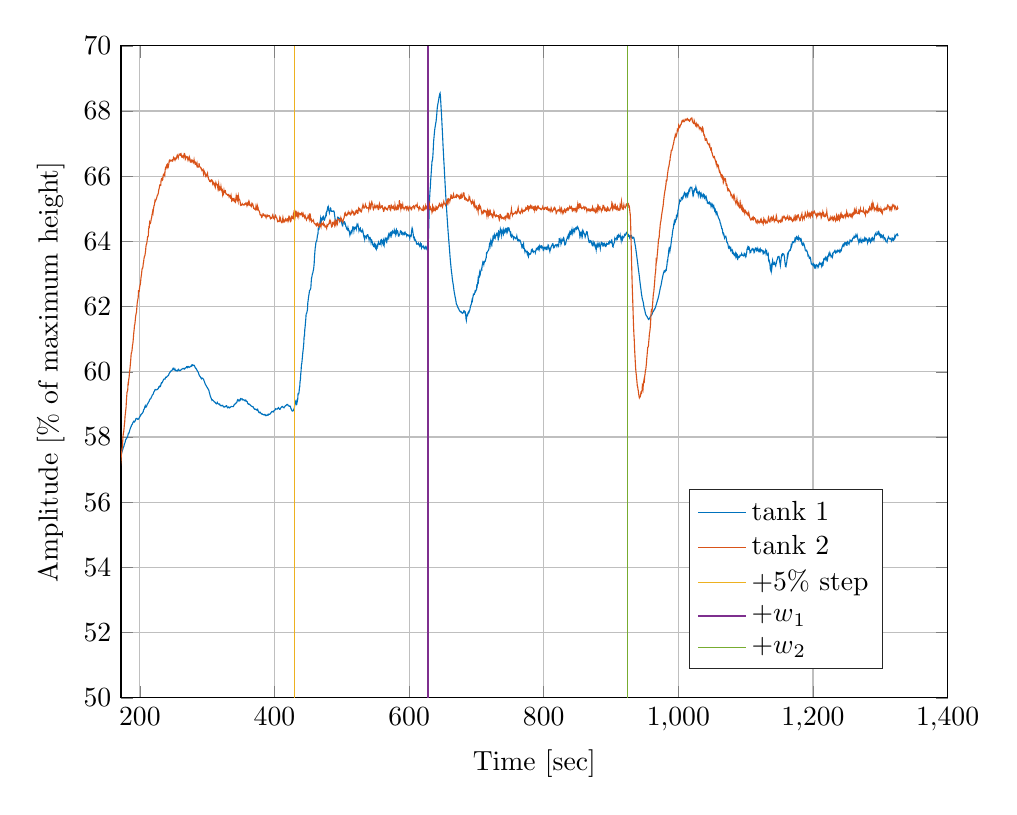
\begin{tikzpicture}

\begin{axis}[%
width=4.133in,
height=3.26in,
at={(0.693in,0.44in)},
scale only axis,
xmin=172,
xmax=1400,
xlabel={Time [sec]},
xmajorgrids,
ymin=50,
ymax=70,
ylabel={Amplitude [$\%$ of maximum height]},
ymajorgrids,
axis background/.style={fill=white},
legend style={at={(0.687,0.044)},anchor=south west,legend cell align=left,align=left,draw=white!15!black}
]
\addplot [color=mycolor1,solid]
  table[row sep=crcr]{%
0	0\\
0.5	6.37086838494614\\
1	8.87018050724773\\
1.5	9.90041293775157\\
2	10.2280940322231\\
2.5	10.3020695925616\\
3	10.3033753948326\\
3.5	10.2870447571123\\
4	10.2727362485081\\
4.5	10.3326531363245\\
5	10.4251998058761\\
5.5	10.7470829453362\\
6	11.2002857199791\\
6.5	11.7331459763235\\
7	12.5354114045817\\
7.5	13.5815785449345\\
8	14.7769954645503\\
8.5	16.027761852635\\
9	17.2894098920943\\
9.5	18.4846025533966\\
10	19.7304143288499\\
10.5	20.9200043735451\\
11	22.0044885161087\\
11.5	23.1254114230498\\
12	24.2128407711278\\
12.5	25.356669265986\\
13	26.4486754088501\\
13.5	27.5645597525778\\
14	28.7099825127061\\
14.5	29.9421524776252\\
15	31.1881891154552\\
15.5	32.3935563383846\\
16	33.6400257785647\\
16.5	34.6138429885366\\
17	35.7056489468352\\
17.5	36.8139894636719\\
18	37.8223913549983\\
18.5	38.8892180208648\\
19	39.8893189322075\\
19.5	40.8089832977934\\
20	41.7118780384786\\
20.5	42.6088496628783\\
21	43.4917031520194\\
21.5	44.4524562515855\\
22	45.3832955742187\\
22.5	46.3305904793534\\
23	47.2912933892248\\
23.5	48.2806063084621\\
24	49.2648425538595\\
24.5	50.2276530181434\\
25	51.2831166272103\\
25.5	52.3181486533861\\
26	53.3320275947761\\
26.5	54.3670195411393\\
27	55.2206096491879\\
27.5	56.0918954206275\\
28	56.8777559432397\\
28.5	57.6725577645916\\
29	58.4180187374056\\
29.5	59.2732591594309\\
30	60.2991144936972\\
30.5	61.8624828249468\\
31	64.1419630909057\\
31.5	65.6574323088567\\
32	66.645133502243\\
32.5	67.2100435703799\\
33	67.6299136620593\\
33.5	67.9484625433785\\
34	68.1922382462525\\
34.5	68.3959776809318\\
35	68.5996013501062\\
35.5	68.7991221915288\\
36	68.8930257918282\\
36.5	68.99371000455\\
37	69.0703983974824\\
37.5	69.1070456527151\\
38	69.1817309846936\\
38.5	69.2304312668921\\
39	69.2407748573722\\
39.5	69.1962920003471\\
40	69.1780608058879\\
40.5	69.1217581342617\\
41	69.0670567526498\\
41.5	69.0185342732204\\
42	68.9404427316898\\
42.5	68.8701409045804\\
43	68.7953946882381\\
43.5	68.6724557424588\\
44	68.585387591916\\
44.5	68.4257726667812\\
45	68.2482921165305\\
45.5	68.1288939254888\\
46	67.9264942763579\\
46.5	67.6521986032064\\
47	67.5317881523442\\
47.5	67.4958702027599\\
48	67.3727160409948\\
48.5	67.2682810639115\\
49	67.0482195412091\\
49.5	66.7172246106823\\
50	66.3317768739943\\
50.5	65.9019594970727\\
51	65.4686429491328\\
51.5	64.9944351180248\\
52	64.4964611777371\\
52.5	63.9727200581048\\
53	63.4770296360872\\
53.5	62.9485157541199\\
54	62.3545719945457\\
54.5	61.7586152953\\
55	61.1555549086955\\
55.5	60.587301285499\\
56	60.0851708777534\\
56.5	59.6077676041866\\
57	59.1301599304939\\
57.5	58.6208022043928\\
58	58.2886076974972\\
58.5	58.3708333953909\\
59	58.5641467343312\\
59.5	58.8339523415672\\
60	59.1705786873173\\
60.5	59.4545561553444\\
61	59.7354237489483\\
61.5	59.9395599873818\\
62	60.1472526357082\\
62.5	60.2815662174188\\
63	60.2645230960031\\
63.5	60.1397650507772\\
64	60.0845469265221\\
64.5	60.0522435827239\\
65	60.1046290915027\\
65.5	59.9821753285592\\
66	59.9510527859412\\
66.5	59.8088219012024\\
67	59.7521695668768\\
67.5	59.6043525870382\\
68	59.4018644100052\\
68.5	59.2050479559305\\
69	59.0254360114208\\
69.5	58.6579017765856\\
70	58.2127005169141\\
70.5	57.7828614650177\\
71	57.3319950627559\\
71.5	56.9094280344418\\
72	56.4436225981927\\
72.5	55.8666719165337\\
73	55.3098645692094\\
73.5	54.8084847484132\\
74	54.321666349058\\
74.5	53.8375904769879\\
75	53.3327633486709\\
75.5	52.8312792692075\\
76	52.3263130179114\\
76.5	51.8407646033233\\
77	51.3872216692564\\
77.5	50.9260823203274\\
78	50.4714551494329\\
78.5	50.0267942574867\\
79	49.6042833164978\\
79.5	49.2072875999696\\
80	48.8351923715029\\
80.5	48.4563611566966\\
81	48.0972656280289\\
81.5	47.762187103102\\
82	47.3844119520126\\
82.5	47.0416580588607\\
83	46.7399721123996\\
83.5	46.4727436996792\\
84	46.1686547885273\\
84.5	45.8753671653944\\
85	45.6380051807598\\
85.5	45.3792843566341\\
86	45.1554112705696\\
86.5	44.9505729570365\\
87	44.7553738274858\\
87.5	44.5492120866355\\
88	44.3733792671021\\
88.5	44.1855099831864\\
89	44.0431245582408\\
89.5	43.8825500326302\\
90	43.7390617246862\\
90.5	43.5708813113296\\
91	43.4594921253461\\
91.5	43.3319814450734\\
92	43.2539593092237\\
92.5	43.1930685150907\\
93	43.1056000873927\\
93.5	42.9993718134127\\
94	42.9077041546672\\
94.5	42.856415322724\\
95	42.8053780662446\\
95.5	42.767562880113\\
96	42.7348591444365\\
96.5	42.6936565142728\\
97	42.6259754147892\\
97.5	42.6309233335067\\
98	42.6132878038538\\
98.5	42.6510269349276\\
99	42.6120056081852\\
99.5	42.6321596135005\\
100	42.6825681133831\\
100.5	42.7224318688817\\
101	42.6975912125772\\
101.5	42.7183373557198\\
102	42.7846547642596\\
102.5	42.8589185323379\\
103	42.9120528582531\\
103.5	42.9788486209107\\
104	43.0723322108116\\
104.5	43.1245285405618\\
105	43.2058062418729\\
105.5	43.3211348556704\\
106	43.3984580323278\\
106.5	43.4739703297531\\
107	43.5370248304745\\
107.5	43.5979235230723\\
108	43.6693119063048\\
108.5	43.7497270083678\\
109	43.82793800136\\
109.5	43.8968611941385\\
110	44.0039897876886\\
110.5	44.0930537538819\\
111	44.1859507669103\\
111.5	44.2878658904687\\
112	44.3589835833724\\
112.5	44.4124330200484\\
113	44.4842970606833\\
113.5	44.6029783994593\\
114	44.6829839170633\\
114.5	44.7930420239677\\
115	44.9339067637442\\
115.5	45.0695907931591\\
116	45.1668045631532\\
116.5	45.2276117877247\\
117	45.3808998406138\\
117.5	45.4545693420436\\
118	45.5518582478339\\
118.5	45.6524528282869\\
119	45.7433967604427\\
119.5	45.8315037501454\\
120	45.9818918193804\\
120.5	46.1598555125573\\
121	46.2601457439155\\
121.5	46.365740494995\\
122	46.4353178137082\\
122.5	46.5242686104884\\
123	46.6331606541114\\
123.5	46.7877280677567\\
124	46.8787997156577\\
124.5	46.9984948561544\\
125	47.1349573814734\\
125.5	47.2417188841762\\
126	47.3369160484893\\
126.5	47.4624214710384\\
127	47.5848815917568\\
127.5	47.6981871689679\\
128	47.8034414721216\\
128.5	47.91955234697\\
129	48.0563766396342\\
129.5	48.1725772447879\\
130	48.3401561689615\\
130.5	48.4674012866583\\
131	48.5955053714373\\
131.5	48.7370177513915\\
132	48.8827462255586\\
132.5	49.0130913047554\\
133	49.117825221172\\
133.5	49.2387217250584\\
134	49.3365543439901\\
134.5	49.454662168035\\
135	49.6014178931984\\
135.5	49.7344255776245\\
136	49.8774952624918\\
136.5	50.0083160331098\\
137	50.1087831935309\\
137.5	50.2159143235472\\
138	50.3641661489764\\
138.5	50.4809470084218\\
139	50.607600559397\\
139.5	50.7669242853232\\
140	50.8834507188203\\
140.5	50.9928098086925\\
141	51.1372006480073\\
141.5	51.2552038420796\\
142	51.3409914326055\\
142.5	51.4618024911584\\
143	51.5786735875217\\
143.5	51.698886971191\\
144	51.8348541133396\\
144.5	51.9892894487069\\
145	52.0946615081458\\
145.5	52.2192445931799\\
146	52.3556351588622\\
146.5	52.4434631129858\\
147	52.5459998130419\\
147.5	52.6994226430164\\
148	52.8543913126717\\
148.5	52.9547944601251\\
149	53.0088643121486\\
149.5	53.1014751105561\\
150	53.1606991079845\\
150.5	53.3217027958115\\
151	53.3899871221097\\
151.5	53.5620197164387\\
152	53.7658007312704\\
152.5	53.9046717655577\\
153	53.9990739242363\\
153.5	54.1257471422933\\
154	54.2622769061193\\
154.5	54.373722005102\\
155	54.4755874075309\\
155.5	54.5811170308809\\
156	54.6835607353858\\
156.5	54.7970568755449\\
157	54.9225033240353\\
157.5	55.0480154436381\\
158	55.1629505584127\\
158.5	55.2693789038995\\
159	55.35987800853\\
159.5	55.49325753979\\
160	55.6270924018232\\
160.5	55.7403810158064\\
161	55.8266522172017\\
161.5	55.9188570057953\\
162	56.0140533442471\\
162.5	56.1123690577729\\
163	56.1873548721937\\
163.5	56.2885818387268\\
164	56.3859612119053\\
164.5	56.4568881585983\\
165	56.5471222929225\\
165.5	56.6219419622754\\
166	56.6984769397766\\
166.5	56.7849033459239\\
167	56.8492084734413\\
167.5	56.9269162552165\\
168	56.9409323243535\\
168.5	56.9995432068442\\
169	57.0876099446355\\
169.5	57.1480314317417\\
170	57.2132920097806\\
170.5	57.2746028823792\\
171	57.3158768185619\\
171.5	57.3919917601439\\
172	57.4082643886449\\
172.5	57.4502374665907\\
173	57.5161865739072\\
173.5	57.5424360518979\\
174	57.5909732241402\\
174.5	57.6051007940199\\
175	57.6535896551344\\
175.5	57.6860097037846\\
176	57.7027508033014\\
176.5	57.7348814966331\\
177	57.7859661356328\\
177.5	57.8091419972695\\
178	57.8268293993821\\
178.5	57.8821776760126\\
179	57.9194094441191\\
179.5	57.9336152674134\\
180	57.9554338356668\\
180.5	57.9670301714292\\
181	57.9792587557357\\
181.5	57.9946924437358\\
182	58.0249237482118\\
182.5	58.0815215979786\\
183	58.1129866097031\\
183.5	58.1097276462247\\
184	58.1292900181407\\
184.5	58.1737683893191\\
185	58.2128946476452\\
185.5	58.2384089288368\\
186	58.2791544236894\\
186.5	58.3023534937596\\
187	58.316237294857\\
187.5	58.351087141966\\
188	58.3734339362996\\
188.5	58.3803181726569\\
189	58.4097688701691\\
189.5	58.433375113936\\
190	58.45033703369\\
190.5	58.4732606026456\\
191	58.4845919262528\\
191.5	58.4782778378914\\
192	58.4641835510518\\
192.5	58.4778211657714\\
193	58.4963789487287\\
193.5	58.518860221249\\
194	58.5526029248266\\
194.5	58.5692385073041\\
195	58.5688181476571\\
195.5	58.5711924253567\\
196	58.5565004967256\\
196.5	58.5454091250816\\
197	58.5398289940716\\
197.5	58.5523208426028\\
198	58.5502000794211\\
198.5	58.5757093484672\\
199	58.5798138863183\\
199.5	58.6163397104116\\
200	58.6158138004592\\
200.5	58.6470676477744\\
201	58.6735168190701\\
201.5	58.6731365029983\\
202	58.6908438763568\\
202.5	58.7104234984819\\
203	58.7141250695965\\
203.5	58.7251520747284\\
204	58.7396039994979\\
204.5	58.7587660599033\\
205	58.7803832248565\\
205.5	58.8271083232944\\
206	58.8444546478567\\
206.5	58.8656806708694\\
207	58.8954406128243\\
207.5	58.9344833141225\\
208	58.9591241775779\\
208.5	58.926598215705\\
209	58.9138773098285\\
209.5	58.9258972167026\\
210	58.9472130407844\\
210.5	58.9699993571446\\
211	59.0022876578616\\
211.5	59.0206802818784\\
212	59.0261605600425\\
212.5	59.0606905777994\\
213	59.0716337658571\\
213.5	59.0850617136625\\
214	59.1085128832733\\
214.5	59.1400348190847\\
215	59.1633087391405\\
215.5	59.1699043807672\\
216	59.1735789078793\\
216.5	59.1938227452833\\
217	59.218336592194\\
217.5	59.2343829593148\\
218	59.2613455142669\\
218.5	59.2882643599472\\
219	59.2964938589159\\
219.5	59.309218386037\\
220	59.3245311189296\\
220.5	59.3647093831735\\
221	59.3892218449909\\
221.5	59.399438516467\\
222	59.4219895366531\\
222.5	59.4552953938342\\
223	59.4573683420889\\
223.5	59.4451854371878\\
224	59.4435568797432\\
224.5	59.4454132068135\\
225	59.4490232365018\\
225.5	59.4586723692144\\
226	59.4582411797061\\
226.5	59.4744017503434\\
227	59.4742953742849\\
227.5	59.4933702792377\\
228	59.5317993024199\\
228.5	59.5282196133071\\
229	59.5440867638518\\
229.5	59.5632207202036\\
230	59.5598795168709\\
230.5	59.5515271986689\\
231	59.584781093026\\
231.5	59.6279540116053\\
232	59.6580207675965\\
232.5	59.651531869328\\
233	59.6606317064036\\
233.5	59.6869109714372\\
234	59.7071650214646\\
234.5	59.7291263898705\\
235	59.7535799349915\\
235.5	59.7746676699178\\
236	59.7735694408971\\
236.5	59.7770221035249\\
237	59.7814224925727\\
237.5	59.7806982337877\\
238	59.8155329184902\\
238.5	59.8348805681195\\
239	59.8295721147987\\
239.5	59.8321004401269\\
240	59.8426888289149\\
240.5	59.8540252848451\\
241	59.8696699771085\\
241.5	59.8755946259283\\
242	59.8779813604927\\
242.5	59.8919837139006\\
243	59.921843903457\\
243.5	59.9507933784416\\
244	59.9612278203412\\
244.5	59.9797832583476\\
245	59.9922467687537\\
245.5	60.0091816850901\\
246	60.0230952712814\\
246.5	60.0198026940993\\
247	60.0250600035843\\
247.5	60.0407179678579\\
248	60.0511893419833\\
248.5	60.0814198671374\\
249	60.089261769473\\
249.5	60.1083745695005\\
250	60.0910499776063\\
250.5	60.065920108629\\
251	60.0570601626292\\
251.5	60.0658149893712\\
252	60.0899935817225\\
252.5	60.0640963677764\\
253	60.0434662619173\\
253.5	60.0334573099383\\
254	60.0406695755585\\
254.5	60.0395309454653\\
255	60.0283340330725\\
255.5	60.0390056680995\\
256	60.0252105954811\\
256.5	60.0311320902376\\
257	60.065514381276\\
257.5	60.0750096571467\\
258	60.0553857476778\\
258.5	60.039719171355\\
259	60.0333860394204\\
259.5	60.0389295077444\\
260	60.035386029705\\
260.5	60.0404508364565\\
261	60.055604704635\\
261.5	60.0736574413501\\
262	60.077811220658\\
262.5	60.0811202268014\\
263	60.0895280701358\\
263.5	60.0885470137322\\
264	60.1001017622455\\
264.5	60.1008593807949\\
265	60.1002773852277\\
265.5	60.1005299059108\\
266	60.0818826815293\\
266.5	60.0895519152366\\
267	60.0933468738165\\
267.5	60.1184312595692\\
268	60.1214866830124\\
268.5	60.1266251733798\\
269	60.1281661244816\\
269.5	60.1591097032856\\
270	60.1610317807983\\
270.5	60.1456759832414\\
271	60.1303166707255\\
271.5	60.1575911041336\\
272	60.1614288076838\\
272.5	60.1462368454381\\
273	60.1465945265983\\
273.5	60.1363359989777\\
274	60.1431938071871\\
274.5	60.1493284391039\\
275	60.1613387278836\\
275.5	60.163830320236\\
276	60.1767269718062\\
276.5	60.188483663035\\
277	60.1776041596052\\
277.5	60.217134488984\\
278	60.2152607043009\\
278.5	60.201672008304\\
279	60.1925961083695\\
279.5	60.1948788619057\\
280	60.2059889201472\\
280.5	60.2047294269092\\
281	60.1878932199637\\
281.5	60.1693392489709\\
282	60.1355616276392\\
282.5	60.1160920207803\\
283	60.1166005228552\\
283.5	60.0893339444536\\
284	60.08667828047\\
284.5	60.0675113279969\\
285	60.0380624358959\\
285.5	60.0263786141956\\
286	60.00279494039\\
286.5	59.9959291930149\\
287	59.9707506272823\\
287.5	59.9324374379592\\
288	59.9063578144264\\
288.5	59.8775015958818\\
289	59.8676569406736\\
289.5	59.8584396873732\\
290	59.8356468528144\\
290.5	59.8149359966796\\
291	59.8049306392556\\
291.5	59.7892557744152\\
292	59.8118666733643\\
292.5	59.8109087206673\\
293	59.7971249879532\\
293.5	59.7943486879825\\
294	59.7831265234398\\
294.5	59.7675413547321\\
295	59.7434028517853\\
295.5	59.715438115768\\
296	59.6942969141765\\
296.5	59.6610059721493\\
297	59.6243395854061\\
297.5	59.6123936237552\\
298	59.5878970193472\\
298.5	59.5777397522435\\
299	59.5493381572357\\
299.5	59.5334562454673\\
300	59.5254364890062\\
300.5	59.5064295041647\\
301	59.4840088781431\\
301.5	59.4692135377778\\
302	59.4532152299533\\
302.5	59.4302065129299\\
303	59.3840274897466\\
303.5	59.3499160828938\\
304	59.3039491590945\\
304.5	59.2658445753124\\
305	59.2358028011217\\
305.5	59.2110768591292\\
306	59.1833691968096\\
306.5	59.157074509664\\
307	59.1302332625585\\
307.5	59.1444495565953\\
308	59.1390030565357\\
308.5	59.1276482418445\\
309	59.1158162960949\\
309.5	59.1034989273122\\
310	59.0950095750823\\
310.5	59.0805211128168\\
311	59.0789722048181\\
311.5	59.0657538619897\\
312	59.0599652877591\\
312.5	59.0389700022332\\
313	59.0345910772599\\
313.5	59.0201003507937\\
314	59.0300863907082\\
314.5	59.0372690431356\\
315	59.0604467026122\\
315.5	59.0424701033509\\
316	59.0207070817723\\
316.5	59.0141273550799\\
317	59.0162730707257\\
317.5	59.0095821157178\\
318	58.9979838970044\\
318.5	59.0078145263172\\
319	58.9759329701594\\
319.5	58.9732931349795\\
320	58.9603088579903\\
320.5	58.9552858907301\\
321	58.9573405435223\\
321.5	58.9577324445908\\
322	58.9720809503186\\
322.5	58.9702341730802\\
323	58.9711212345861\\
323.5	58.9501512747316\\
324	58.927166638555\\
324.5	58.9222672420336\\
325	58.9315577601141\\
325.5	58.9180670323852\\
326	58.9180375737707\\
326.5	58.9263281964785\\
327	58.9385797619259\\
327.5	58.9406715409002\\
328	58.9524832524284\\
328.5	58.959064612572\\
329	58.9563725924261\\
329.5	58.9183225910945\\
330	58.9098174025981\\
330.5	58.8968887941718\\
331	58.9104526755552\\
331.5	58.9188046319046\\
332	58.9219604702581\\
332.5	58.8977515741442\\
333	58.892299167234\\
333.5	58.9041904970594\\
334	58.9044107943686\\
334.5	58.9107524887384\\
335	58.9261817204823\\
335.5	58.9294467324853\\
336	58.9296870552004\\
336.5	58.9387433921936\\
337	58.933765407598\\
337.5	58.9302407728758\\
338	58.9329314205281\\
338.5	58.9318189515448\\
339	58.9316709527081\\
339.5	58.9621145286637\\
340	58.9847981045359\\
340.5	58.9940830204288\\
341	59.0050035076703\\
341.5	59.0157925627685\\
342	59.0217599856363\\
342.5	59.0243832909175\\
343	59.0502495049643\\
343.5	59.0541273019362\\
344	59.0597251539915\\
344.5	59.0996715781796\\
345	59.1319976430075\\
345.5	59.1463911618145\\
346	59.1273168626161\\
346.5	59.1113217988595\\
347	59.1046700479127\\
347.5	59.1281240132137\\
348	59.1124891829399\\
348.5	59.1119176452961\\
349	59.1259479285563\\
349.5	59.1785214813174\\
350	59.1813744156757\\
350.5	59.1687850640797\\
351	59.1686295838991\\
351.5	59.166638391369\\
352	59.1426550703037\\
352.5	59.1603063739898\\
353	59.1493036001811\\
353.5	59.1449483763368\\
354	59.1374569516857\\
354.5	59.1393723548756\\
355	59.1263323626822\\
355.5	59.1168392946728\\
356	59.1104778706411\\
356.5	59.111924878065\\
357	59.132779283891\\
357.5	59.1289181862396\\
358	59.0957150347162\\
358.5	59.0963764332514\\
359	59.0946531358055\\
359.5	59.0756734201293\\
360	59.0378618021644\\
360.5	59.0317484795729\\
361	59.0110020118176\\
361.5	59.0060392753606\\
362	59.0150100858054\\
362.5	59.0089220345086\\
363	59.0008634943793\\
363.5	58.9847781690952\\
364	58.9819102206067\\
364.5	58.966607143688\\
365	58.9546871554631\\
365.5	58.9530747509111\\
366	58.9467259624627\\
366.5	58.9366118211664\\
367	58.9296692203405\\
367.5	58.926477379913\\
368	58.9278363038815\\
368.5	58.9200614907148\\
369	58.8927749442512\\
369.5	58.8782559560392\\
370	58.8612125751924\\
370.5	58.8532154631993\\
371	58.8585695567015\\
371.5	58.847370101516\\
372	58.8406499327166\\
372.5	58.8426422120727\\
373	58.8467525272932\\
373.5	58.842696448899\\
374	58.8192393747111\\
374.5	58.822591750146\\
375	58.8443691225837\\
375.5	58.8159784355226\\
376	58.7843307360454\\
376.5	58.7641475155852\\
377	58.7502240318119\\
377.5	58.7427863704297\\
378	58.7539634034895\\
378.5	58.7629038293393\\
379	58.7587479934376\\
379.5	58.7368179660797\\
380	58.7218956251353\\
380.5	58.7161596677466\\
381	58.7058598469419\\
381.5	58.6980434733248\\
382	58.7071776683929\\
382.5	58.6969664154921\\
383	58.6919326491682\\
383.5	58.6862658458504\\
384	58.6805851901362\\
384.5	58.675861787872\\
385	58.685275607223\\
385.5	58.6942910581028\\
386	58.6906296882748\\
386.5	58.6636718863193\\
387	58.6539856931359\\
387.5	58.6573830949796\\
388	58.6566028676985\\
388.5	58.6672709500302\\
389	58.6778133652121\\
389.5	58.6788942724148\\
390	58.6712779564963\\
390.5	58.6935116852481\\
391	58.681369245682\\
391.5	58.6976823914098\\
392	58.6953789781294\\
392.5	58.6940664339266\\
393	58.6985617844083\\
393.5	58.7096588700265\\
394	58.7136848742755\\
394.5	58.738227299874\\
395	58.7520873098434\\
395.5	58.7628553289529\\
396	58.7779568255989\\
396.5	58.7852206917369\\
397	58.783014326213\\
397.5	58.7765062233903\\
398	58.7667196366187\\
398.5	58.792506481703\\
399	58.7955077918608\\
399.5	58.809011926765\\
400	58.8180212008059\\
400.5	58.8258456002046\\
401	58.831331989907\\
401.5	58.8642990254186\\
402	58.8553438626614\\
402.5	58.8569391232522\\
403	58.8587977191625\\
403.5	58.8579805061356\\
404	58.8544256791403\\
404.5	58.8728254582627\\
405	58.8805408105519\\
405.5	58.8861921874688\\
406	58.8979395996284\\
406.5	58.8770892640395\\
407	58.8621034037343\\
407.5	58.846380315768\\
408	58.8453301609157\\
408.5	58.8570970768371\\
409	58.8787786079876\\
409.5	58.8974084323029\\
410	58.9069909053624\\
410.5	58.9211176947769\\
411	58.9240905871763\\
411.5	58.9375622816226\\
412	58.9347097228275\\
412.5	58.9149066947333\\
413	58.9116655741913\\
413.5	58.905917432088\\
414	58.8953467225838\\
414.5	58.9181860606279\\
415	58.9219252741389\\
415.5	58.9388942918525\\
416	58.9570298382139\\
416.5	58.9597437596685\\
417	58.9624980397903\\
417.5	58.976450229645\\
418	58.9844602384223\\
418.5	58.9992665778498\\
419	59.002054106003\\
419.5	58.9999700515018\\
420	58.9803013378319\\
420.5	58.9554221010138\\
421	58.951883223347\\
421.5	58.9547080390466\\
422	58.9425761608829\\
422.5	58.9433044209052\\
423	58.9480729376464\\
423.5	58.939850964948\\
424	58.9072954006567\\
424.5	58.8652583732278\\
425	58.8561565743805\\
425.5	58.8332171587319\\
426	58.8013444476857\\
426.5	58.7981613777759\\
427	58.7980132582342\\
427.5	58.8039206799377\\
428	58.809714696617\\
428.5	58.8386742964011\\
429	58.8613127562921\\
429.5	58.8997565220139\\
430	58.9633785756779\\
430.5	58.9995723256233\\
431	59.0340938625343\\
431.5	59.0827355855792\\
432	59.0531051460463\\
432.5	59.0230123548786\\
433	59.0881515508838\\
433.5	59.0560435618643\\
434	59.1137082761567\\
434.5	59.1585914466516\\
435	59.3264496951669\\
435.5	59.3213422691867\\
436	59.3221774007192\\
436.5	59.3816022870591\\
437	59.496441908948\\
437.5	59.5455740162374\\
438	59.7091090730007\\
438.5	59.7584059499477\\
439	59.9399627850661\\
439.5	60.0315933985066\\
440	60.2085796176458\\
440.5	60.2529408636172\\
441	60.3476726625452\\
441.5	60.4603530470042\\
442	60.580796701702\\
442.5	60.6610814055601\\
443	60.7643719622476\\
443.5	60.8751571138553\\
444	61.0873239298068\\
444.5	61.0949023282002\\
445	61.2962192253592\\
445.5	61.3756903421013\\
446	61.5110209192302\\
446.5	61.623784472676\\
447	61.7724042441802\\
447.5	61.7840978095839\\
448	61.8122261356081\\
448.5	61.8588107479932\\
449	61.9142063801469\\
449.5	62.1217810228019\\
450	62.1874316292945\\
450.5	62.2794995330097\\
451	62.3478667530109\\
451.5	62.4055774911946\\
452	62.4920846180457\\
452.5	62.5013117412532\\
453	62.5118475267883\\
453.5	62.54280694024\\
454	62.5766084570856\\
454.5	62.7483608481598\\
455	62.8698419357442\\
455.5	62.908457372457\\
456	62.9711367301277\\
456.5	63.0147208889632\\
457	63.0387015345742\\
457.5	63.0953977024717\\
458	63.1374773103005\\
458.5	63.2248635334659\\
459	63.3445374461594\\
459.5	63.5506155081693\\
460	63.6803665354315\\
460.5	63.8052268385329\\
461	63.8542141675311\\
461.5	63.9754186597598\\
462	63.9869591500559\\
462.5	63.9991861778001\\
463	64.0548524266537\\
463.5	64.1287928410796\\
464	64.205163032298\\
464.5	64.2138319210563\\
465	64.3778201604938\\
465.5	64.3568813523601\\
466	64.368445465696\\
466.5	64.443102504064\\
467	64.4574435763273\\
467.5	64.5817299886125\\
468	64.6332576868812\\
468.5	64.7018567340235\\
469	64.6141380854831\\
469.5	64.663240357197\\
470	64.6366231543924\\
470.5	64.6674525018808\\
471	64.7149104072977\\
471.5	64.6914263070525\\
472	64.734963667734\\
472.5	64.7589679344627\\
473	64.7195873310508\\
473.5	64.6609203207234\\
474	64.6511945716566\\
474.5	64.6700825339084\\
475	64.7117135260402\\
475.5	64.764644720126\\
476	64.7574982355352\\
476.5	64.8429848583382\\
477	64.820789259295\\
477.5	64.9186127433626\\
478	64.9194214939659\\
478.5	64.9760362935672\\
479	65.0329263470865\\
479.5	65.0083196959611\\
480	65.0465549143163\\
480.5	64.950752837688\\
481	64.9397657897438\\
481.5	64.8825953533566\\
482	64.9358296812873\\
482.5	64.9437701221622\\
483	65.0240130321585\\
483.5	65.0141969141365\\
484	64.9459698256309\\
484.5	64.9204782292981\\
485	64.9191376341178\\
485.5	64.930915561629\\
486	64.9270426779391\\
486.5	64.9242240381246\\
487	64.9212115017401\\
487.5	64.9349269850854\\
488	64.9330702962736\\
488.5	64.9190803959513\\
489	64.8499383669068\\
489.5	64.7726235093043\\
490	64.6903113007396\\
490.5	64.6174066144937\\
491	64.5456979783654\\
491.5	64.5593615769355\\
492	64.5925221282986\\
492.5	64.6424523989383\\
493	64.6371683843315\\
493.5	64.7036965084201\\
494	64.6791066936107\\
494.5	64.7368591103101\\
495	64.7351298383208\\
495.5	64.695072691804\\
496	64.7014631174476\\
496.5	64.6435120402065\\
497	64.6925610574039\\
497.5	64.6838803857855\\
498	64.6628708194401\\
498.5	64.6538786013079\\
499	64.632976618426\\
499.5	64.5845933400741\\
500	64.5505210443406\\
500.5	64.5090858214965\\
501	64.5361733547508\\
501.5	64.5020427009289\\
502	64.5532419808218\\
502.5	64.5704286772023\\
503	64.6009750192267\\
503.5	64.6045058687987\\
504	64.600090468333\\
504.5	64.5385668687263\\
505	64.5489415243029\\
505.5	64.5118513628294\\
506	64.4573945117892\\
506.5	64.4459821433957\\
507	64.3975715966924\\
507.5	64.3733035554518\\
508	64.3614078611389\\
508.5	64.3789544197961\\
509	64.4200719147154\\
509.5	64.3515333151017\\
510	64.368417262514\\
510.5	64.3354970597992\\
511	64.314379500415\\
511.5	64.2511814468694\\
512	64.1908127423162\\
512.5	64.2281635702651\\
513	64.2330076702518\\
513.5	64.3013626688544\\
514	64.3257077332508\\
514.5	64.3333674010619\\
515	64.2845003978892\\
515.5	64.3429469334252\\
516	64.398733450178\\
516.5	64.4466219972033\\
517	64.4406174307814\\
517.5	64.4320236170536\\
518	64.3360278547554\\
518.5	64.4067623284566\\
519	64.393947183605\\
519.5	64.4341475196862\\
520	64.4377815209488\\
520.5	64.4088965938247\\
521	64.4234502703754\\
521.5	64.3818592527673\\
522	64.4578486854536\\
522.5	64.5073384492714\\
523	64.4681483692057\\
523.5	64.4793100520162\\
524	64.5121243881096\\
524.5	64.4601385981052\\
525	64.4150817189293\\
525.5	64.3180993523849\\
526	64.3474262606704\\
526.5	64.3491305934086\\
527	64.3845435646268\\
527.5	64.4028469195126\\
528	64.3243458475063\\
528.5	64.300919059853\\
529	64.292981962943\\
529.5	64.3129409150942\\
530	64.2907911664798\\
530.5	64.3021439481529\\
531	64.3389408356442\\
531.5	64.2932504667445\\
532	64.2339325552493\\
532.5	64.1704912588082\\
533	64.1300595195049\\
533.5	64.149121135831\\
534	64.073557825031\\
534.5	64.1423157597431\\
535	64.1404479315807\\
535.5	64.162323329663\\
536	64.1587412054888\\
536.5	64.1234378992055\\
537	64.1722584304593\\
537.5	64.1725683658852\\
538	64.2086095697438\\
538.5	64.2084934635628\\
539	64.1892233803334\\
539.5	64.1156179575584\\
540	64.1194819152442\\
540.5	64.0500732290945\\
541	64.1132650516105\\
541.5	64.1207016870803\\
542	64.1217539489754\\
542.5	64.0761171313313\\
543	64.0509786201274\\
543.5	63.958823669892\\
544	64.0031735416786\\
544.5	64.027949068107\\
545	63.9847848383462\\
545.5	63.9799895070526\\
546	63.8975288721554\\
546.5	63.8741370076576\\
547	63.8562084835302\\
547.5	63.8899794238959\\
548	63.8687112472758\\
548.5	63.906685274194\\
549	63.8518903025361\\
549.5	63.8721601507415\\
550	63.8223281303326\\
550.5	63.8714569226226\\
551	63.8128829286553\\
551.5	63.7720776087765\\
552	63.8265231824404\\
552.5	63.811944906857\\
553	63.884377041477\\
553.5	63.8702224354012\\
554	63.9323153259118\\
554.5	63.9742055105265\\
555	63.9413148571546\\
555.5	63.9307434272507\\
556	63.9105908187038\\
556.5	63.9207855940278\\
557	63.9102985145671\\
557.5	63.979434624899\\
558	64.0386016120737\\
558.5	64.0482220001011\\
559	64.0555397081005\\
559.5	63.945591832457\\
560	64.0075444208136\\
560.5	64.0143666055982\\
561	63.9862797252969\\
561.5	63.9358476804148\\
562	64.0214572799381\\
562.5	63.972067632601\\
563	63.9116950177332\\
563.5	64.0247147318632\\
564	64.043594385381\\
564.5	64.0923841807057\\
565	64.0698755846431\\
565.5	64.0803233379231\\
566	64.0150165071648\\
566.5	64.0571057049707\\
567	64.0155421887841\\
567.5	64.0806097115518\\
568	64.0770263202769\\
568.5	64.1374165654225\\
569	64.178757199489\\
569.5	64.209046736519\\
570	64.132033451437\\
570.5	64.1809660662578\\
571	64.1887180924861\\
571.5	64.2283156060017\\
572	64.1905231721557\\
572.5	64.2639978551708\\
573	64.2824842727683\\
573.5	64.2723358290357\\
574	64.2049790076243\\
574.5	64.2713164488293\\
575	64.254587324879\\
575.5	64.3079537921333\\
576	64.2822151327297\\
576.5	64.2625392828193\\
577	64.2574795122009\\
577.5	64.2540677566395\\
578	64.3454035992389\\
578.5	64.3079002332908\\
579	64.3077520113239\\
579.5	64.2346528034714\\
580	64.3133883852069\\
580.5	64.3370115891097\\
581	64.3606704225205\\
581.5	64.2658016145246\\
582	64.306714455273\\
582.5	64.3263158966052\\
583	64.3173390887071\\
583.5	64.2520594221669\\
584	64.185921392233\\
584.5	64.2025368152933\\
585	64.1790474649265\\
585.5	64.208798117007\\
586	64.2098834630826\\
586.5	64.2587986493971\\
587	64.3100051307759\\
587.5	64.2955396051133\\
588	64.3101494893812\\
588.5	64.2988040816086\\
589	64.2232523267283\\
589.5	64.2286591935618\\
590	64.2301184157481\\
590.5	64.2532132341581\\
591	64.2057846285437\\
591.5	64.2191982004337\\
592	64.2213637815869\\
592.5	64.2491575814433\\
593	64.2234760468994\\
593.5	64.2553352169351\\
594	64.2777084166097\\
594.5	64.2470937595608\\
595	64.2236722195505\\
595.5	64.2100966194249\\
596	64.2206672274941\\
596.5	64.1686662535929\\
597	64.1914262371518\\
597.5	64.2030215703927\\
598	64.1798546138691\\
598.5	64.1866057621846\\
599	64.1748144960609\\
599.5	64.1877412773296\\
600	64.1729548760708\\
600.5	64.1612925851193\\
601	64.1043711820674\\
601.5	64.174841677676\\
602	64.1579598129958\\
602.5	64.1612736788604\\
603	64.1533532547661\\
603.5	64.280807406912\\
604	64.3588030359467\\
604.5	64.4106673262465\\
605	64.3786065679916\\
605.5	64.2915140419024\\
606	64.2309679966571\\
606.5	64.1257060735745\\
607	64.1104993567155\\
607.5	64.0704579214065\\
608	64.1033437531511\\
608.5	64.068055473047\\
609	64.0371380956437\\
609.5	64.0407829132125\\
610	64.0059868946864\\
610.5	63.9962307410428\\
611	63.9285789906954\\
611.5	63.9406518040781\\
612	63.9295853725158\\
612.5	63.9279292033905\\
613	63.9107484391864\\
613.5	63.9143835225479\\
614	63.9391639373727\\
614.5	63.8988982955658\\
615	63.9068494795401\\
615.5	63.8735619396772\\
616	63.8456178092476\\
616.5	63.8688470652742\\
617	63.9333533843732\\
617.5	63.9074448644096\\
618	63.9162632750665\\
618.5	63.8196402766122\\
619	63.860216974815\\
619.5	63.839124134297\\
620	63.8346545662646\\
620.5	63.8299774023591\\
621	63.8207232519039\\
621.5	63.8432471823653\\
622	63.7890696043042\\
622.5	63.7725729846997\\
623	63.7775671945191\\
623.5	63.7689877676686\\
624	63.8245677873195\\
624.5	63.8220706703317\\
625	63.8421084768962\\
625.5	63.8186269683081\\
626	63.7768534238079\\
626.5	63.7514708344808\\
627	63.7675030078231\\
627.5	63.7779819243832\\
628	63.7241559813709\\
628.5	63.9159570605907\\
629	64.3411790414143\\
629.5	64.7356040691483\\
630	65.092928373511\\
630.5	65.3432920236134\\
631	65.5367694920949\\
631.5	65.6688443630738\\
632	65.8684501636887\\
632.5	65.9991739969878\\
633	66.1616499536043\\
633.5	66.3069876402612\\
634	66.4640750202061\\
634.5	66.4768403251445\\
635	66.5477962058766\\
635.5	66.6998342567381\\
636	66.9016233243219\\
636.5	67.0947388350535\\
637	67.2011397074532\\
637.5	67.317137412974\\
638	67.421277963555\\
638.5	67.4933208629655\\
639	67.5518752126396\\
639.5	67.626230078514\\
640	67.6695751892865\\
640.5	67.77839088321\\
641	67.880967474301\\
641.5	68.0253717590268\\
642	68.1281290635358\\
642.5	68.1925326278428\\
643	68.2451592126666\\
643.5	68.3005570575361\\
644	68.3548020775032\\
644.5	68.4300834421156\\
645	68.4751458653885\\
645.5	68.5228780587023\\
646	68.5476614398193\\
646.5	68.4555971336569\\
647	68.2753083873562\\
647.5	68.0911366973773\\
648	67.9322884331559\\
648.5	67.7317149541012\\
649	67.5250435346407\\
649.5	67.3231596666262\\
650	67.1090657208926\\
650.5	66.8843821263236\\
651	66.6925115540878\\
651.5	66.4919507221803\\
652	66.3241194448734\\
652.5	66.1194239468731\\
653	65.9250900496677\\
653.5	65.7417641335426\\
654	65.5450904051816\\
654.5	65.365465512247\\
655	65.2025869194755\\
655.5	65.0372187016792\\
656	64.8838429956277\\
656.5	64.7190275354078\\
657	64.5723050598259\\
657.5	64.4172127730871\\
658	64.2734648011403\\
658.5	64.1485976037701\\
659	64.010056837538\\
659.5	63.8842748444055\\
660	63.7521835863385\\
660.5	63.6084634646378\\
661	63.4795937446874\\
661.5	63.3582212467964\\
662	63.2567398264139\\
662.5	63.1510496897843\\
663	63.052369094112\\
663.5	62.9904556097491\\
664	62.8810695086662\\
664.5	62.7992464027919\\
665	62.7329825189164\\
665.5	62.6756332665354\\
666	62.598085653457\\
666.5	62.5158238724958\\
667	62.4470847760544\\
667.5	62.3913780907315\\
668	62.3321772893376\\
668.5	62.2826124645924\\
669	62.2315007427768\\
669.5	62.1758003408724\\
670	62.0977717705092\\
670.5	62.0616948741384\\
671	62.0534814674849\\
671.5	62.0325646506634\\
672	61.9928798138887\\
672.5	61.9650412187324\\
673	61.9578035880691\\
673.5	61.9418428582126\\
674	61.9096547176015\\
674.5	61.8871801206263\\
675	61.874589751853\\
675.5	61.8541010358117\\
676	61.8427028402136\\
676.5	61.8528609899584\\
677	61.8528469646619\\
677.5	61.8264910185614\\
678	61.8080775953286\\
678.5	61.8104544838853\\
679	61.8054191794053\\
679.5	61.7948774550317\\
680	61.8130275095154\\
680.5	61.8183180399519\\
681	61.85747471228\\
681.5	61.874330617418\\
682	61.8671779444928\\
682.5	61.8402478826974\\
683	61.8061218176902\\
683.5	61.8200266091092\\
684	61.7594957183205\\
684.5	61.6353449783577\\
685	61.5832455753517\\
685.5	61.682890362666\\
686	61.7464540141323\\
686.5	61.7611970607113\\
687	61.744502946708\\
687.5	61.8089129647786\\
688	61.8032812317379\\
688.5	61.8424396092177\\
689	61.8293289882302\\
689.5	61.8715480904476\\
690	61.8878683147123\\
690.5	61.9248356872781\\
691	62.0023986273188\\
691.5	62.0300315823882\\
692	62.054261087667\\
692.5	62.0787236807997\\
693	62.1549509327963\\
693.5	62.204715488956\\
694	62.1815309475044\\
694.5	62.2646655429889\\
695	62.3052662221386\\
695.5	62.3741773266467\\
696	62.3634919497897\\
696.5	62.3777175247871\\
697	62.3773256428743\\
697.5	62.4207360732572\\
698	62.4715218412489\\
698.5	62.4543027248255\\
699	62.4746205918481\\
699.5	62.5037863454643\\
700	62.512607273699\\
700.5	62.6323978875603\\
701	62.6127166440124\\
701.5	62.6854222142062\\
702	62.7409982116975\\
702.5	62.8467793568383\\
703	62.7950690957684\\
703.5	62.9105672517425\\
704	62.9251997039924\\
704.5	63.0194204754817\\
705	62.9426882359884\\
705.5	62.9660185505348\\
706	63.0618952331535\\
706.5	63.0802879285362\\
707	63.1292786585875\\
707.5	63.158439368349\\
708	63.1444159977401\\
708.5	63.2635815737659\\
709	63.290699163135\\
709.5	63.3603394423838\\
710	63.3425803066874\\
710.5	63.358194313623\\
711	63.3028116574658\\
711.5	63.3728886933123\\
712	63.3626433428891\\
712.5	63.3942781669888\\
713	63.3924543288196\\
713.5	63.4247643496\\
714	63.4729417562413\\
714.5	63.4986925789735\\
715	63.638952665591\\
715.5	63.6303161142634\\
716	63.6666650201648\\
716.5	63.687659470256\\
717	63.7010186820561\\
717.5	63.7165533490768\\
718	63.7246218210371\\
718.5	63.7703084524944\\
719	63.8331184713272\\
719.5	63.9353286977267\\
720	63.9270656798601\\
720.5	63.9402913524446\\
721	63.9941496162258\\
721.5	63.8746270363605\\
722	63.9235566952887\\
722.5	63.9654099114933\\
723	63.9260057406021\\
723.5	64.0390492635787\\
724	64.0205528376126\\
724.5	64.1175424165613\\
725	64.086749129699\\
725.5	64.1660432224922\\
726	64.1656202756244\\
726.5	64.2024767486395\\
727	64.1311411305005\\
727.5	64.1588535466046\\
728	64.1143886053946\\
728.5	64.1565128879263\\
729	64.1818882006364\\
729.5	64.2130768815617\\
730	64.1984893538178\\
730.5	64.2393294651465\\
731	64.2116088158783\\
731.5	64.1976946875877\\
732	64.1201364292925\\
732.5	64.221392858271\\
733	64.155711822602\\
733.5	64.2481618278549\\
734	64.201948242961\\
734.5	64.2608108197921\\
735	64.2930545835087\\
735.5	64.3772474131667\\
736	64.3358145571418\\
736.5	64.2905914088598\\
737	64.199472702116\\
737.5	64.3023658736394\\
738	64.2669274735104\\
738.5	64.2746708779891\\
739	64.3146298723429\\
739.5	64.2476231680587\\
740	64.3292041623874\\
740.5	64.2553272530694\\
741	64.2991052913133\\
741.5	64.2813349050594\\
742	64.3332097673753\\
742.5	64.317669475599\\
743	64.3775578586576\\
743.5	64.3571641354389\\
744	64.3049430808767\\
744.5	64.382188327919\\
745	64.3842370393625\\
745.5	64.4005781799624\\
746	64.298493839271\\
746.5	64.3294218830726\\
747	64.3518864680737\\
747.5	64.3897658859124\\
748	64.4144841577899\\
748.5	64.4088430389799\\
749	64.317891525147\\
749.5	64.3181072541831\\
750	64.2993068882853\\
750.5	64.2218984280861\\
751	64.2471470292229\\
751.5	64.1451674233197\\
752	64.132666578462\\
752.5	64.1762329488148\\
753	64.1972001282394\\
753.5	64.1640918874783\\
754	64.1677304004436\\
754.5	64.143938300576\\
755	64.0882456296469\\
755.5	64.1236413169577\\
756	64.1373640619593\\
756.5	64.1313477274562\\
757	64.1209816397491\\
757.5	64.0975504557589\\
758	64.1018988074057\\
758.5	64.0839085043726\\
759	64.1028110757193\\
759.5	64.1145446089924\\
760	64.1636697682883\\
760.5	64.1092352644606\\
761	64.0465102965966\\
761.5	64.0574654980376\\
762	64.0209975348732\\
762.5	64.0492194313023\\
763	64.0546958512116\\
763.5	64.0450212956875\\
764	64.023470446348\\
764.5	64.0069358347325\\
765	64.0213617716102\\
765.5	63.9907760178928\\
766	63.9640661526284\\
766.5	63.9066439976567\\
767	63.9017709776423\\
767.5	63.8240611474646\\
768	63.8424631644591\\
768.5	63.8712088268387\\
769	63.8313896041112\\
769.5	63.8847038423811\\
770	63.9234416183373\\
770.5	63.788062232564\\
771	63.7889481700138\\
771.5	63.7358729656424\\
772	63.6869471293186\\
772.5	63.735523323362\\
773	63.731664951003\\
773.5	63.702859601551\\
774	63.6951961875286\\
774.5	63.6733240531202\\
775	63.6662726842454\\
775.5	63.6162007652832\\
776	63.6721391308302\\
776.5	63.6509425241128\\
777	63.6534084238052\\
777.5	63.5545880579154\\
778	63.6008354839083\\
778.5	63.6079812931989\\
779	63.6192650832942\\
779.5	63.6057252608174\\
780	63.6072135551816\\
780.5	63.62734231806\\
781	63.6428801654326\\
781.5	63.7166633662679\\
782	63.7052587955399\\
782.5	63.7558750999585\\
783	63.7619319847223\\
783.5	63.7077638590121\\
784	63.6816022028433\\
784.5	63.6669338966782\\
785	63.6981674005752\\
785.5	63.6915297678578\\
786	63.6887756520291\\
786.5	63.6940384991686\\
787	63.6992843612552\\
787.5	63.6564141817709\\
788	63.7066362299061\\
788.5	63.7302797788886\\
789	63.7782839656862\\
789.5	63.7649788538467\\
790	63.7506471388251\\
790.5	63.7702972474368\\
791	63.8031419370381\\
791.5	63.8185483829861\\
792	63.7749030183186\\
792.5	63.8204267568102\\
793	63.7988978929911\\
793.5	63.8443182138639\\
794	63.7844908954726\\
794.5	63.8550169386769\\
795	63.856696927351\\
795.5	63.8357805192557\\
796	63.8491151059085\\
796.5	63.8188968165729\\
797	63.8594038343136\\
797.5	63.8532780750084\\
798	63.8180129619995\\
798.5	63.8020073850206\\
799	63.7546869290681\\
799.5	63.7826634789291\\
800	63.7552642093366\\
800.5	63.8228047772645\\
801	63.8212182150162\\
801.5	63.7799070836391\\
802	63.7766714724459\\
802.5	63.7721059271893\\
803	63.7991506274769\\
803.5	63.7457165940304\\
804	63.7457352640089\\
804.5	63.7921968649094\\
805	63.7725198841215\\
805.5	63.8309774150407\\
806	63.8326206718671\\
806.5	63.8918398110716\\
807	63.8805852524094\\
807.5	63.7824929038435\\
808	63.7544574278847\\
808.5	63.7334994851355\\
809	63.6942242923056\\
809.5	63.7672237889706\\
810	63.7505134352377\\
810.5	63.7774748265289\\
811	63.8416334343109\\
811.5	63.85026220301\\
812	63.8801413827868\\
812.5	63.8943426739388\\
813	63.923755422205\\
813.5	63.9303637069987\\
814	63.8926412871478\\
814.5	63.8083462541952\\
815	63.8185517602756\\
815.5	63.810832078754\\
816	63.825782781167\\
816.5	63.8732537821826\\
817	63.8716886930754\\
817.5	63.8881957363066\\
818	63.8747766120073\\
818.5	63.8729968866575\\
819	63.8874674186818\\
819.5	63.8516234013464\\
820	63.8968387553808\\
820.5	63.9055239926078\\
821	63.894809940226\\
821.5	63.8801144561182\\
822	63.8596336178418\\
822.5	63.9467038314677\\
823	64.073660829222\\
823.5	64.0678275182662\\
824	64.0810686175695\\
824.5	63.9993664933194\\
825	64.0126588971511\\
825.5	63.9337119380922\\
826	63.9918248729886\\
826.5	63.9699157697075\\
827	64.0390005669498\\
827.5	64.0095123399357\\
828	64.0149524925681\\
828.5	64.0190983987041\\
829	64.0966528889305\\
829.5	64.1135470337573\\
830	64.0807313543378\\
830.5	64.0160319851732\\
831	63.9244804752744\\
831.5	63.8910551601994\\
832	63.9017311809184\\
832.5	63.9202371436517\\
833	63.977794593679\\
833.5	64.0206026733291\\
834	64.0588546525001\\
834.5	64.0793509043657\\
835	64.1235271309987\\
835.5	64.1135559078606\\
836	64.1588366060022\\
836.5	64.121044681824\\
837	64.1966939436787\\
837.5	64.234540383265\\
838	64.2558950370412\\
838.5	64.1886677471255\\
839	64.2731099803242\\
839.5	64.2455140931881\\
840	64.2789561863336\\
840.5	64.247420523833\\
841	64.3069633752531\\
841.5	64.2783109964011\\
842	64.3486601895234\\
842.5	64.2693824416897\\
843	64.3335335781568\\
843.5	64.3170314033624\\
844	64.3211837730597\\
844.5	64.3542967006529\\
845	64.2866179745703\\
845.5	64.3248359032947\\
846	64.3117953755342\\
846.5	64.3928971874151\\
847	64.3894460818859\\
847.5	64.4140735938027\\
848	64.4234568805531\\
848.5	64.3760123691337\\
849	64.3913700096506\\
849.5	64.3911772337563\\
850	64.4425200148609\\
850.5	64.4198516285944\\
851	64.4258129805478\\
851.5	64.373980652763\\
852	64.3560073207979\\
852.5	64.3351838292836\\
853	64.2886222810561\\
853.5	64.1854002029962\\
854	64.2503331502218\\
854.5	64.2175474007666\\
855	64.2427981150795\\
855.5	64.1638234069721\\
856	64.2202656056674\\
856.5	64.241893715393\\
857	64.2897070411476\\
857.5	64.1888952347214\\
858	64.2563828981832\\
858.5	64.31598649419\\
859	64.2875633289291\\
859.5	64.2566676481653\\
860	64.2457127906286\\
860.5	64.2168165327246\\
861	64.1904759860263\\
861.5	64.1368681284349\\
862	64.1785120980315\\
862.5	64.2153875362887\\
863	64.2438920175827\\
863.5	64.2847972488434\\
864	64.2992982602595\\
864.5	64.2926941096246\\
865	64.1986264060338\\
865.5	64.1739778660102\\
866	64.0984392751976\\
866.5	64.0563110232135\\
867	63.9969980757999\\
867.5	63.9660713826118\\
868	63.9633693279862\\
868.5	63.9630876171307\\
869	64.0215598131908\\
869.5	64.0122655283314\\
870	64.0125321067546\\
870.5	63.995356143272\\
871	63.9515892599024\\
871.5	63.9748724693884\\
872	63.8777853107347\\
872.5	63.8665927971746\\
873	63.8618410425977\\
873.5	63.9312943510135\\
874	63.9189856579776\\
874.5	63.9832707276693\\
875	63.9640727330804\\
875.5	63.9112785483464\\
876	63.8526017453678\\
876.5	63.8352360218618\\
877	63.8004004469957\\
877.5	63.8542598124683\\
878	63.7565470165398\\
878.5	63.8372592175497\\
879	63.8263973783796\\
879.5	63.8876567362032\\
880	63.8724265293891\\
880.5	63.9281350928576\\
881	63.8622479262227\\
881.5	63.8964456063221\\
882	63.8796961638208\\
882.5	63.9160991695058\\
883	63.8662694018004\\
883.5	63.8476088939126\\
884	63.7844064327002\\
884.5	63.8775112674486\\
885	63.91721525097\\
885.5	63.9689044446448\\
886	63.952919801946\\
886.5	63.9202742444562\\
887	63.8924828851853\\
887.5	63.9448082214811\\
888	63.9357878443807\\
888.5	63.9085865981416\\
889	63.8797361817467\\
889.5	63.9128183641406\\
890	63.945431578529\\
890.5	63.939931115272\\
891	63.879548529824\\
891.5	63.8478892573475\\
892	63.8416665840629\\
892.5	63.8868776305508\\
893	63.8796876245815\\
893.5	63.9367415178512\\
894	63.927075672702\\
894.5	63.9231732166257\\
895	63.9196061445222\\
895.5	63.9107224305047\\
896	63.9176842026429\\
896.5	63.9724820457545\\
897	63.9886119434337\\
897.5	63.9997175399347\\
898	63.9535683204984\\
898.5	63.9867543884988\\
899	63.9813656652524\\
899.5	63.9757920801371\\
900	63.9658771956674\\
900.5	64.0341768460199\\
901	64.0456325363855\\
901.5	63.988363938052\\
902	63.9069249472266\\
902.5	63.8431116163259\\
903	63.8324718754899\\
903.5	63.9099912567137\\
904	63.9155535048709\\
904.5	63.9567933967783\\
905	63.9603558379903\\
905.5	64.0815390022102\\
906	64.0533382089087\\
906.5	64.084944414215\\
907	64.0770311113716\\
907.5	64.0784044599701\\
908	64.098932721113\\
908.5	64.0652190481215\\
909	64.1320837071232\\
909.5	64.1041880683473\\
910	64.1619123818596\\
910.5	64.1445196439311\\
911	64.1865581698949\\
911.5	64.1557518294691\\
912	64.1773946111408\\
912.5	64.176125565516\\
913	64.1518011662522\\
913.5	64.1944646353659\\
914	64.1161699264033\\
914.5	64.0910087133115\\
915	64.0271023611038\\
915.5	64.1139515446384\\
916	64.1362634875409\\
916.5	64.1139461531318\\
917	64.0681780834165\\
917.5	64.1321761295066\\
918	64.108986823403\\
918.5	64.1265451069207\\
919	64.1248844060009\\
919.5	64.1515946796557\\
920	64.1999033588848\\
920.5	64.1793914250155\\
921	64.1782245684498\\
921.5	64.2212076080262\\
922	64.2192909471726\\
922.5	64.2582176561578\\
923	64.2701900900021\\
923.5	64.237852436736\\
924	64.2306918360073\\
924.5	64.2176830884049\\
925	64.1820344424372\\
925.5	64.1676517022365\\
926	64.1994788930642\\
926.5	64.1810158108509\\
927	64.1747759274062\\
927.5	64.1268955220258\\
928	64.1665600458323\\
928.5	64.1710062767512\\
929	64.1541915320176\\
929.5	64.1698690421079\\
930	64.1393785221581\\
930.5	64.1634752180601\\
931	64.1356726387907\\
931.5	64.1090217410643\\
932	64.0999442156969\\
932.5	64.1131661324134\\
933	64.1233677229732\\
933.5	64.1260861174192\\
934	64.1059293840981\\
934.5	64.0426093082308\\
935	63.9861000369689\\
935.5	63.9267701751773\\
936	63.8714274282485\\
936.5	63.8072684380006\\
937	63.7314098835093\\
937.5	63.6559757718582\\
938	63.5788837377067\\
938.5	63.4923022402458\\
939	63.4146886440227\\
939.5	63.3411350081375\\
940	63.2481681504483\\
940.5	63.1640291046323\\
941	63.0865826330583\\
941.5	63.0122694453934\\
942	62.9317674116902\\
942.5	62.8345149063385\\
943	62.7484749119073\\
943.5	62.6609316062629\\
944	62.5862063942686\\
944.5	62.5140915471976\\
945	62.4104469837132\\
945.5	62.3484224115327\\
946	62.2883390295659\\
946.5	62.2303237776873\\
947	62.1924376530095\\
947.5	62.1541221481225\\
948	62.1098602011211\\
948.5	62.0333553026496\\
949	61.9765114516199\\
949.5	61.9198784691444\\
950	61.8975911547909\\
950.5	61.8472759909582\\
951	61.7977988180425\\
951.5	61.7590008705563\\
952	61.7362562024216\\
952.5	61.7199728655669\\
953	61.7047450978392\\
953.5	61.69812384417\\
954	61.6645148135788\\
954.5	61.6547046547993\\
955	61.6330102454263\\
955.5	61.6084745366533\\
956	61.6025138711116\\
956.5	61.6242565738285\\
957	61.6362845427582\\
957.5	61.6540263393426\\
958	61.6701938496128\\
958.5	61.7036349468153\\
959	61.7117432314419\\
959.5	61.7196061250851\\
960	61.7342399547423\\
960.5	61.7476575027332\\
961	61.770945055208\\
961.5	61.8200614686142\\
962	61.8338809249096\\
962.5	61.8356867831574\\
963	61.8604770283908\\
963.5	61.8782029324167\\
964	61.9063960569703\\
964.5	61.90648118822\\
965	61.9409885696632\\
965.5	61.9546128774881\\
966	61.9771416058373\\
966.5	62.0161490544023\\
967	62.0564778735824\\
967.5	62.0863003896589\\
968	62.1207994687335\\
968.5	62.1547090219374\\
969	62.1969187107824\\
969.5	62.2239330122137\\
970	62.2607517355903\\
970.5	62.304067904287\\
971	62.3431505282498\\
971.5	62.3980650514402\\
972	62.4499770158904\\
972.5	62.4987350060072\\
973	62.5634620706258\\
973.5	62.6056557678715\\
974	62.6318141426189\\
974.5	62.6866816188642\\
975	62.7378416466083\\
975.5	62.8067194201054\\
976	62.8466156685651\\
976.5	62.9057311860889\\
977	62.9492341319232\\
977.5	62.9974951259824\\
978	63.0342462916913\\
978.5	63.0634937418704\\
979	63.0962132130939\\
979.5	63.0917738979978\\
980	63.0717670072278\\
980.5	63.1063511622981\\
981	63.0975664510045\\
981.5	63.1297573066859\\
982	63.1213468625946\\
982.5	63.2084300719355\\
983	63.2731942104444\\
983.5	63.3894072241939\\
984	63.3843870393125\\
984.5	63.5124768411886\\
985	63.5572685317518\\
985.5	63.6666723927107\\
986	63.7650008408748\\
986.5	63.8077519136489\\
987	63.791732733295\\
987.5	63.71805029473\\
988	63.7844285042965\\
988.5	63.8270250176136\\
989	63.9135304679398\\
989.5	63.9925765486402\\
990	64.1110843879555\\
990.5	64.1291359628036\\
991	64.2277826770303\\
991.5	64.3052276278321\\
992	64.3816060853842\\
992.5	64.3974503743736\\
993	64.5148804336175\\
993.5	64.5515154757829\\
994	64.6111425284072\\
994.5	64.5580643618604\\
995	64.5941592096099\\
995.5	64.5953050935199\\
996	64.6696039718255\\
996.5	64.6699157338295\\
997	64.7562956292808\\
997.5	64.7159090207338\\
998	64.7467208896813\\
998.5	64.7773992234757\\
999	64.8550265648221\\
999.5	64.9587890565057\\
1000	64.9908947480668\\
1000.5	65.0778563313981\\
1001	65.1377246601509\\
1001.5	65.1761452575807\\
1002	65.2540091175187\\
1002.5	65.2314656761733\\
1003	65.2278648402649\\
1003.5	65.2439122186927\\
1004	65.2628798823017\\
1004.5	65.3491729666257\\
1005	65.3511547915256\\
1005.5	65.3516908626854\\
1006	65.3178764762752\\
1006.5	65.3608233061587\\
1007	65.3421233188177\\
1007.5	65.3888671961789\\
1008	65.4104384952914\\
1008.5	65.4631933647354\\
1009	65.4881605028197\\
1009.5	65.4468781627572\\
1010	65.456658358711\\
1010.5	65.3890797856217\\
1011	65.4257218394405\\
1011.5	65.461390729766\\
1012	65.4347722672979\\
1012.5	65.3907832271048\\
1013	65.441469046693\\
1013.5	65.4656921517651\\
1014	65.4137497495671\\
1014.5	65.4765316421987\\
1015	65.4693939045965\\
1015.5	65.5622987072924\\
1016	65.5974545989729\\
1016.5	65.606223703847\\
1017	65.5727005187736\\
1017.5	65.654597721896\\
1018	65.6593293670678\\
1018.5	65.6642678742578\\
1019	65.6474768312694\\
1019.5	65.6407260251788\\
1020	65.6480877519742\\
1020.5	65.5671586301767\\
1021	65.5163562729293\\
1021.5	65.4427785387841\\
1022	65.4847058359341\\
1022.5	65.4443577116389\\
1023	65.5442867331185\\
1023.5	65.5339277880087\\
1024	65.5907161938057\\
1024.5	65.5756489061539\\
1025	65.594178984489\\
1025.5	65.6122184613445\\
1026	65.6692277704244\\
1026.5	65.6232913219394\\
1027	65.5397068686237\\
1027.5	65.5618318102061\\
1028	65.4965235922382\\
1028.5	65.5025532966484\\
1029	65.4851277028975\\
1029.5	65.4224801994549\\
1030	65.5076808592905\\
1030.5	65.5129875782175\\
1031	65.5257759769638\\
1031.5	65.4724121339012\\
1032	65.4571402920462\\
1032.5	65.3890979490102\\
1033	65.4399759617239\\
1033.5	65.3962277841937\\
1034	65.4525822248049\\
1034.5	65.4135258888523\\
1035	65.4304956093756\\
1035.5	65.4011653033216\\
1036	65.4099745947267\\
1036.5	65.3615450174185\\
1037	65.3988033785289\\
1037.5	65.4400059219413\\
1038	65.4189998128574\\
1038.5	65.4213010189417\\
1039	65.3406722023999\\
1039.5	65.3640113770252\\
1040	65.3600368644711\\
1040.5	65.3745723250873\\
1041	65.313470647315\\
1041.5	65.3482169568211\\
1042	65.2989241268672\\
1042.5	65.2518599885999\\
1043	65.1932962779563\\
1043.5	65.2101840262523\\
1044	65.1774124060121\\
1044.5	65.1649098149261\\
1045	65.1763833161691\\
1045.5	65.1544411191337\\
1046	65.1508380529268\\
1046.5	65.198867515806\\
1047	65.1850751233189\\
1047.5	65.149151951895\\
1048	65.1333963863349\\
1048.5	65.0763696234948\\
1049	65.1191086457209\\
1049.5	65.1003444699039\\
1050	65.1483338067676\\
1050.5	65.1236049269143\\
1051	65.0778978459852\\
1051.5	65.0361552859772\\
1052	65.0655837592393\\
1052.5	65.0916792118416\\
1053	65.0369538606586\\
1053.5	65.0157959823124\\
1054	64.9278406448284\\
1054.5	64.9108647750038\\
1055	64.9597474056664\\
1055.5	64.9253792201597\\
1056	64.8637728514009\\
1056.5	64.9101166290041\\
1057	64.9101903980729\\
1057.5	64.8681850322744\\
1058	64.8093938186989\\
1058.5	64.7992598112625\\
1059	64.7555905778942\\
1059.5	64.72305835104\\
1060	64.7081792014833\\
1060.5	64.6785166230957\\
1061	64.6624643322669\\
1061.5	64.6325194983508\\
1062	64.5689884673477\\
1062.5	64.5563684678231\\
1063	64.5241409625455\\
1063.5	64.4631600234505\\
1064	64.4501751403415\\
1064.5	64.3889531682808\\
1065	64.3881866184022\\
1065.5	64.3410350957803\\
1066	64.2638919916354\\
1066.5	64.224838362026\\
1067	64.2480742788258\\
1067.5	64.2261923424916\\
1068	64.1659243162873\\
1068.5	64.1092761975007\\
1069	64.1419587970648\\
1069.5	64.1508237976489\\
1070	64.1389323039738\\
1070.5	64.1502114287935\\
1071	64.113536829378\\
1071.5	64.0431745461183\\
1072	63.9756085488508\\
1072.5	63.9764901433372\\
1073	63.9445627384719\\
1073.5	63.9251896088248\\
1074	63.8648358105688\\
1074.5	63.8086883667984\\
1075	63.788881439394\\
1075.5	63.8097327095006\\
1076	63.8334082919009\\
1076.5	63.7996604737994\\
1077	63.784974685645\\
1077.5	63.739499814834\\
1078	63.780024689115\\
1078.5	63.7284463787194\\
1079	63.7322265579601\\
1079.5	63.7201367538357\\
1080	63.6706818051486\\
1080.5	63.7071828752584\\
1081	63.6495335378537\\
1081.5	63.6573771087265\\
1082	63.6112587969422\\
1082.5	63.5974798592862\\
1083	63.5746947905816\\
1083.5	63.6012017868141\\
1084	63.6201746982967\\
1084.5	63.5869573431731\\
1085	63.6258797148412\\
1085.5	63.5287259755253\\
1086	63.5608555909904\\
1086.5	63.595934289598\\
1087	63.5546648090535\\
1087.5	63.5020064971336\\
1088	63.5438028944327\\
1088.5	63.488639691452\\
1089	63.5321879550846\\
1089.5	63.5355294987288\\
1090	63.5057310373999\\
1090.5	63.5104982293013\\
1091	63.5407450336882\\
1091.5	63.5685344962897\\
1092	63.5534756082566\\
1092.5	63.5597338904447\\
1093	63.5852250067211\\
1093.5	63.5837818323787\\
1094	63.6194765235375\\
1094.5	63.5719904917118\\
1095	63.5718459382076\\
1095.5	63.5808516283323\\
1096	63.5712219859019\\
1096.5	63.5526474448055\\
1097	63.5580364542346\\
1097.5	63.5839353926909\\
1098	63.6351607215627\\
1098.5	63.629605109044\\
1099	63.5851740986597\\
1099.5	63.5319498650058\\
1100	63.5557831537784\\
1100.5	63.5442085274058\\
1101	63.6173033264855\\
1101.5	63.6561165828954\\
1102	63.758817746702\\
1102.5	63.7902747008341\\
1103	63.7782003572804\\
1103.5	63.8415494138858\\
1104	63.8282782009657\\
1104.5	63.7848179510836\\
1105	63.8128236704946\\
1105.5	63.7856474175697\\
1106	63.7331020356103\\
1106.5	63.6538986150481\\
1107	63.668244327983\\
1107.5	63.6656307808575\\
1108	63.7201553411144\\
1108.5	63.7295681547558\\
1109	63.7442374197699\\
1109.5	63.7675535407611\\
1110	63.7415901791016\\
1110.5	63.7493372662941\\
1111	63.76869305817\\
1111.5	63.753424302284\\
1112	63.706244141032\\
1112.5	63.6578343746049\\
1113	63.6751469500626\\
1113.5	63.7161349143117\\
1114	63.7700756325454\\
1114.5	63.797591588965\\
1115	63.8003664658705\\
1115.5	63.7715781264525\\
1116	63.7342386376\\
1116.5	63.7570646794212\\
1117	63.7193216974953\\
1117.5	63.7339401074097\\
1118	63.7769924231588\\
1118.5	63.7257069451597\\
1119	63.709106956452\\
1119.5	63.7265286493017\\
1120	63.6814230205015\\
1120.5	63.6929964049498\\
1121	63.7656838105255\\
1121.5	63.7793598513448\\
1122	63.7160638722704\\
1122.5	63.7454548906342\\
1123	63.7423783321422\\
1123.5	63.7184575933075\\
1124	63.7297745382954\\
1124.5	63.7141610553834\\
1125	63.7188274603174\\
1125.5	63.6868524710099\\
1126	63.6176611428445\\
1126.5	63.6253778679261\\
1127	63.676656600469\\
1127.5	63.6462994586434\\
1128	63.6703630772741\\
1128.5	63.6771954001992\\
1129	63.6828713844244\\
1129.5	63.7202904262855\\
1130	63.6525737250673\\
1130.5	63.7181122792928\\
1131	63.7237810112153\\
1131.5	63.6307356993838\\
1132	63.5909774430715\\
1132.5	63.6023141224886\\
1133	63.5761656696923\\
1133.5	63.6042993733411\\
1134	63.4326944617767\\
1134.5	63.3910922995398\\
1135	63.406532030662\\
1135.5	63.3558641917208\\
1136	63.3148661280602\\
1136.5	63.154334796552\\
1137	63.1220865310729\\
1137.5	63.211779260184\\
1138	63.2488696061076\\
1138.5	63.1213430997791\\
1139	63.2008135800303\\
1139.5	63.3399998351129\\
1140	63.4122850192456\\
1140.5	63.3577030622111\\
1141	63.2912917461524\\
1141.5	63.2903344247532\\
1142	63.304119328206\\
1142.5	63.3311989700791\\
1143	63.3486614434396\\
1143.5	63.2872882739853\\
1144	63.2797303233924\\
1144.5	63.2537655819374\\
1145	63.3074507302266\\
1145.5	63.3219469514322\\
1146	63.3897338623239\\
1146.5	63.43265686328\\
1147	63.4472438967335\\
1147.5	63.5022867798483\\
1148	63.5315542302455\\
1148.5	63.5337058407602\\
1149	63.540364963536\\
1149.5	63.538106284387\\
1150	63.46627890645\\
1150.5	63.370010070265\\
1151	63.3316932494633\\
1151.5	63.2620906424035\\
1152	63.3498373531595\\
1152.5	63.4361179467978\\
1153	63.5265354174796\\
1153.5	63.5752352656631\\
1154	63.5548384603801\\
1154.5	63.5707333251326\\
1155	63.6226909935443\\
1155.5	63.6165198930684\\
1156	63.6169928764503\\
1156.5	63.6124459454313\\
1157	63.5822958846962\\
1157.5	63.5290473654231\\
1158	63.412798978605\\
1158.5	63.3262013104985\\
1159	63.2538383680867\\
1159.5	63.2759104473088\\
1160	63.2511410797473\\
1160.5	63.3140121559107\\
1161	63.3543013972386\\
1161.5	63.4634728397582\\
1162	63.5785822455433\\
1162.5	63.5406597222871\\
1163	63.5948635132412\\
1163.5	63.6478174886436\\
1164	63.6858476276243\\
1164.5	63.6982972287431\\
1165	63.7282580101258\\
1165.5	63.7362445315345\\
1166	63.7236821617484\\
1166.5	63.7338390101144\\
1167	63.7954626038684\\
1167.5	63.8713917891818\\
1168	63.8385217149245\\
1168.5	63.8709203338816\\
1169	63.9329578924953\\
1169.5	63.9868803605368\\
1170	63.985923032891\\
1170.5	63.9778826126191\\
1171	63.9879892965877\\
1171.5	63.9682362537235\\
1172	63.9983459112913\\
1172.5	64.0045644486814\\
1173	64.056321707948\\
1173.5	64.020091765223\\
1174	64.0691059150765\\
1174.5	64.1185434335079\\
1175	64.125576455104\\
1175.5	64.1404095215408\\
1176	64.0933170005769\\
1176.5	64.0560562463505\\
1177	64.0606352667298\\
1177.5	64.1133746175701\\
1178	64.1406303513416\\
1178.5	64.0614052982925\\
1179	64.0785379787936\\
1179.5	64.0750765202528\\
1180	64.0962269157382\\
1180.5	64.0739616056381\\
1181	64.0398736762522\\
1181.5	64.0789204417874\\
1182	64.0872775659057\\
1182.5	64.0552938826951\\
1183	63.9956549945099\\
1183.5	63.9143513371116\\
1184	63.8996679016395\\
1184.5	63.9238649560778\\
1185	63.892507287043\\
1185.5	63.9133324307951\\
1186	63.9386351506456\\
1186.5	63.920346296889\\
1187	63.881484154497\\
1187.5	63.8305229390434\\
1188	63.8110962027948\\
1188.5	63.7301570212618\\
1189	63.7292751054219\\
1189.5	63.7107227360893\\
1190	63.7206696851883\\
1190.5	63.730134496456\\
1191	63.6929343468249\\
1191.5	63.6734844667397\\
1192	63.6383124528975\\
1192.5	63.5660542239119\\
1193	63.5811425632343\\
1193.5	63.56419889923\\
1194	63.5292576633147\\
1194.5	63.4903626609682\\
1195	63.5048800975739\\
1195.5	63.4849136887261\\
1196	63.4988335104889\\
1196.5	63.4585741275981\\
1197	63.3744444744606\\
1197.5	63.3151771206688\\
1198	63.31963217111\\
1198.5	63.2882783326637\\
1199	63.2961484714033\\
1199.5	63.2945017277551\\
1200	63.2729307173078\\
1200.5	63.3118570373335\\
1201	63.2920222425908\\
1201.5	63.2809968573587\\
1202	63.2217420673816\\
1202.5	63.25182120538\\
1203	63.1947366431863\\
1203.5	63.1995724964407\\
1204	63.1855230634901\\
1204.5	63.2748065454141\\
1205	63.2838144302023\\
1205.5	63.2664758251224\\
1206	63.247303633441\\
1206.5	63.2357622279831\\
1207	63.2519600568171\\
1207.5	63.2015205722938\\
1208	63.224684155331\\
1208.5	63.2437680391109\\
1209	63.3090917913908\\
1209.5	63.3034782169703\\
1210	63.3387415755954\\
1210.5	63.3164292093622\\
1211	63.3071188965299\\
1211.5	63.3216843000436\\
1212	63.3222993720702\\
1212.5	63.2536942030036\\
1213	63.2974236915093\\
1213.5	63.3260868505961\\
1214	63.2774532846472\\
1214.5	63.3185951567666\\
1215	63.2983423225032\\
1215.5	63.372390598137\\
1216	63.4577386874728\\
1216.5	63.4735301070713\\
1217	63.4805645302945\\
1217.5	63.4528796382856\\
1218	63.4367149054758\\
1218.5	63.4680081524218\\
1219	63.5138496985787\\
1219.5	63.4919277160412\\
1220	63.4664508222075\\
1220.5	63.4305543712754\\
1221	63.4808066786936\\
1221.5	63.4433491259408\\
1222	63.4978173401165\\
1222.5	63.5643711753181\\
1223	63.5700918415526\\
1223.5	63.6108398095032\\
1224	63.5759071733361\\
1224.5	63.6036835637083\\
1225	63.6513238493306\\
1225.5	63.6173002693937\\
1226	63.57610035609\\
1226.5	63.5595042114598\\
1227	63.5208359879481\\
1227.5	63.533526603632\\
1228	63.5350467077665\\
1228.5	63.5736156742616\\
1229	63.5291741811703\\
1229.5	63.5842081433527\\
1230	63.6600854452636\\
1230.5	63.6664092111263\\
1231	63.6666332135852\\
1231.5	63.6791190469343\\
1232	63.6957461780429\\
1232.5	63.7177647085119\\
1233	63.68538828317\\
1233.5	63.6500004884073\\
1234	63.667660793998\\
1234.5	63.6979025349726\\
1235	63.703206330727\\
1235.5	63.6741155617758\\
1236	63.6993026404038\\
1236.5	63.7206453599059\\
1237	63.6988498934619\\
1237.5	63.7265948897455\\
1238	63.7251837743668\\
1238.5	63.7083572535457\\
1239	63.6963834584622\\
1239.5	63.6762649926384\\
1240	63.7232311080454\\
1240.5	63.6943013157157\\
1241	63.7302120568679\\
1241.5	63.7251765619461\\
1242	63.7157668723415\\
1242.5	63.7759170911927\\
1243	63.8069122533921\\
1243.5	63.8492533587581\\
1244	63.8732724352539\\
1244.5	63.8674221138267\\
1245	63.9104743621103\\
1245.5	63.9004522181452\\
1246	63.8662016329913\\
1246.5	63.9033854483996\\
1247	63.948777946878\\
1247.5	63.9349591530793\\
1248	63.9488495889797\\
1248.5	63.9299548283563\\
1249	63.9414371621901\\
1249.5	63.8843686225517\\
1250	63.8896865375596\\
1250.5	63.8854171956962\\
1251	63.9854213551036\\
1251.5	63.995732299406\\
1252	63.9545135822925\\
1252.5	63.9460167345266\\
1253	63.930492176124\\
1253.5	63.9141056269677\\
1254	63.9688169224036\\
1254.5	63.9678879203979\\
1255	64.0402493209261\\
1255.5	64.0279370360286\\
1256	64.0215483230814\\
1256.5	64.0265794149298\\
1257	64.0042935136169\\
1257.5	64.0262979551807\\
1258	64.0171210418909\\
1258.5	64.0618398463161\\
1259	64.0910851321602\\
1259.5	64.09535923517\\
1260	64.1148018894567\\
1260.5	64.1078652017892\\
1261	64.1490145809532\\
1261.5	64.1210063353784\\
1262	64.1445776226893\\
1262.5	64.137383289935\\
1263	64.1342535734221\\
1263.5	64.1776971513214\\
1264	64.1329744024523\\
1264.5	64.1377616528829\\
1265	64.1484818083515\\
1265.5	64.196455630321\\
1266	64.1476218389453\\
1266.5	64.0887004967721\\
1267	64.0367001889339\\
1267.5	64.0409999120858\\
1268	63.9717554352351\\
1268.5	64.0227995151807\\
1269	64.0471672763704\\
1269.5	64.0007229948273\\
1270	64.0168881950542\\
1270.5	64.0126803644193\\
1271	64.0570250339947\\
1271.5	63.9821992632189\\
1272	63.9917268942245\\
1272.5	63.9707289578033\\
1273	64.0355340231232\\
1273.5	64.0430648678397\\
1274	64.0591275641888\\
1274.5	64.0133829649459\\
1275	64.0032731648807\\
1275.5	64.0127000729058\\
1276	64.010795693026\\
1276.5	64.0696510916149\\
1277	64.0157907574324\\
1277.5	64.0258472313451\\
1278	64.0655362324492\\
1278.5	64.1000922384534\\
1279	64.0858918678033\\
1279.5	64.0780069926267\\
1280	64.0331860211517\\
1280.5	64.0293605117635\\
1281	63.9675561712974\\
1281.5	64.0223480210261\\
1282	64.0016150993704\\
1282.5	64.0357151333962\\
1283	64.0723310263759\\
1283.5	64.043451017832\\
1284	64.0694785635687\\
1284.5	64.0056172102376\\
1285	64.0033625170437\\
1285.5	63.9774626017873\\
1286	64.0418592557896\\
1286.5	64.0683168837054\\
1287	64.0084830970455\\
1287.5	64.011590218159\\
1288	64.0585917268327\\
1288.5	64.1055844375032\\
1289	64.0884462009037\\
1289.5	64.0557700371574\\
1290	64.0589311622694\\
1290.5	64.0284204229299\\
1291	64.0931384250007\\
1291.5	64.182083344132\\
1292	64.1996265172008\\
1292.5	64.2278040426112\\
1293	64.2401794220015\\
1293.5	64.2607762723231\\
1294	64.1952889253135\\
1294.5	64.2079214969381\\
1295	64.2116264032322\\
1295.5	64.2156148102876\\
1296	64.2246399724925\\
1296.5	64.2890309445144\\
1297	64.3008254409665\\
1297.5	64.2453293205126\\
1298	64.2755040505787\\
1298.5	64.2370830347564\\
1299	64.1913235237663\\
1299.5	64.1734272029527\\
1300	64.1517401672317\\
1300.5	64.1862584481534\\
1301	64.1410777071695\\
1301.5	64.1745806557604\\
1302	64.1894044905637\\
1302.5	64.1519012290436\\
1303	64.126229692807\\
1303.5	64.1515355876346\\
1304	64.1553620361291\\
1304.5	64.1804209899637\\
1305	64.1401454460621\\
1305.5	64.0809787959149\\
1306	64.1138872577988\\
1306.5	64.1088191431084\\
1307	64.0954686311593\\
1307.5	64.0730834042586\\
1308	64.014335146165\\
1308.5	63.9922231010708\\
1309	63.9989523219009\\
1309.5	64.0050191819345\\
1310	63.9802660012453\\
1310.5	64.0366272750015\\
1311	64.0779284072167\\
1311.5	64.0955972772655\\
1312	64.1356261977839\\
1312.5	64.1134448878186\\
1313	64.1075321508921\\
1313.5	64.0847823576293\\
1314	64.0707405172989\\
1314.5	64.0699020961149\\
1315	64.0707089366589\\
1315.5	64.0951752962643\\
1316	64.0987323774499\\
1316.5	64.0093975151429\\
1317	64.0268762831527\\
1317.5	64.0478466294147\\
1318	64.0593349514475\\
1318.5	64.0973653335371\\
1319	64.0844002675297\\
1319.5	64.0288217682253\\
1320	64.038837313873\\
1320.5	64.0614232138849\\
1321	64.1127759100307\\
1321.5	64.1605498843961\\
1322	64.117014538141\\
1322.5	64.1453193672762\\
1323	64.1780924486261\\
1323.5	64.1897775029749\\
1324	64.2178813605458\\
1324.5	64.2190738945023\\
1325	64.2071287686194\\
1325.5	64.2184852224212\\
1326	64.1746878620562\\
1326.5	64.1591933090069\\
};
\addlegendentry{tank 1};

\addplot [color=mycolor2,solid]
  table[row sep=crcr]{%
0	0\\
0.5	9.53154487284067\\
1	13.0397637128306\\
1.5	14.4307973972865\\
2	14.9764568932629\\
2.5	15.2226856860972\\
3	15.3379858678706\\
3.5	15.406030084185\\
4	15.4360616136929\\
4.5	15.4412594964047\\
5	15.4421478409298\\
5.5	15.4430950699535\\
6	15.7795108701778\\
6.5	16.0916420231023\\
7	16.2636749403092\\
7.5	16.3885471550494\\
8	16.5226963828868\\
8.5	16.5322377029809\\
9	16.754568018671\\
9.5	17.2113901841236\\
10	17.7307910464199\\
10.5	18.315562317093\\
11	18.9418848249193\\
11.5	19.6122728481083\\
12	20.3023872671405\\
12.5	21.0926380537815\\
13	21.7625503537944\\
13.5	22.5663622197035\\
14	23.378438877353\\
14.5	24.0386013027001\\
15	24.8615728190258\\
15.5	25.6616157152552\\
16	26.4803510417857\\
16.5	27.3174498501647\\
17	28.0622602186735\\
17.5	28.4371311309829\\
18	28.6316435734775\\
18.5	28.7460665424267\\
19	28.8144760818332\\
19.5	28.7275859545366\\
20	28.4659519646954\\
20.5	28.0777319085992\\
21	27.6466254573924\\
21.5	27.3052802749587\\
22	27.0590216763078\\
22.5	26.8080355797605\\
23	26.63273851984\\
23.5	26.4181640147905\\
24	26.1979364465616\\
24.5	26.004205863724\\
25	25.8402599016668\\
25.5	25.6901803895552\\
26	25.5423506923049\\
26.5	25.3641981975422\\
27	25.2217944489751\\
27.5	25.0552766930559\\
28	24.968575700382\\
28.5	24.8761770879635\\
29	24.7493104214105\\
29.5	24.5739632177437\\
30	24.2953064920349\\
30.5	24.0224915111641\\
31	23.7448345629386\\
31.5	23.495666276301\\
32	23.2195229408229\\
32.5	22.8140817771739\\
33	22.2705096250756\\
33.5	21.6809562991641\\
34	21.101232526617\\
34.5	20.534757170473\\
35	19.9860199424964\\
35.5	19.4755132968618\\
36	18.9842753624273\\
36.5	18.5399556413976\\
37	18.1420690588753\\
37.5	17.7917656351649\\
38	17.5058768734744\\
38.5	17.3641851869987\\
39	17.2959267306831\\
39.5	17.3451370562135\\
40	17.372387080999\\
40.5	17.3916664375143\\
41	17.3942619612034\\
41.5	17.4122749516525\\
42	17.4572475875273\\
42.5	17.5356928628815\\
43	17.5811901292995\\
43.5	17.5515605971902\\
44	17.4926223231189\\
44.5	17.4748859825595\\
45	17.3972378472938\\
45.5	17.2371730358805\\
46	16.9042254028696\\
46.5	16.5122810866394\\
47	16.2223625937496\\
47.5	16.098532552913\\
48	16.0859888551298\\
48.5	16.2147153837193\\
49	16.3306227996185\\
49.5	16.4108625155623\\
50	16.4489806313964\\
50.5	16.4911545919459\\
51	16.5126426999913\\
51.5	16.4396755580427\\
52	16.4085090371443\\
52.5	16.4234261271843\\
53	16.4208468333434\\
53.5	16.4119338190597\\
54	16.3436408150811\\
54.5	16.2552843562076\\
55	16.2312728239452\\
55.5	16.212753071717\\
56	16.1512313363757\\
56.5	16.0773614171633\\
57	16.0447737362387\\
57.5	16.0467310115556\\
58	16.009208438484\\
58.5	15.9829587718547\\
59	15.96951430177\\
59.5	15.9715168998599\\
60	15.9648855239098\\
60.5	15.9655656608268\\
61	15.963678040909\\
61.5	15.9633874972527\\
62	15.9586326488705\\
62.5	15.9562116802187\\
63	16.0951562953893\\
63.5	16.3960862106831\\
64	16.6779887524227\\
64.5	16.823940027735\\
65	16.8416544767167\\
65.5	16.6439574931182\\
66	16.4399229378276\\
66.5	16.5541426495452\\
67	16.8451872784764\\
67.5	17.0991382283777\\
68	17.199366673757\\
68.5	17.3524197321132\\
69	17.5015244992066\\
69.5	17.6648211799229\\
70	17.9464008386492\\
70.5	18.1923712518771\\
71	18.4625575226771\\
71.5	18.7814889433976\\
72	19.1101558358252\\
72.5	19.4102940430864\\
73	19.6211270342848\\
73.5	19.9960033054054\\
74	20.2973861680255\\
74.5	20.6639761231748\\
75	20.8457584571906\\
75.5	21.4815831016563\\
76	21.819775098138\\
76.5	22.0826421970659\\
77	22.4929586081719\\
77.5	22.9039607637329\\
78	23.4992578102892\\
78.5	23.8407480641565\\
79	24.0959795835254\\
79.5	24.2993192219225\\
80	24.574984984425\\
80.5	24.6925563559987\\
81	24.8710859257995\\
81.5	25.0886170543335\\
82	25.5219613535997\\
82.5	25.9618551985495\\
83	26.4314508180197\\
83.5	26.4967794754406\\
84	26.7230650064138\\
84.5	26.8102112741863\\
85	26.9375995159639\\
85.5	27.112552588542\\
86	27.2812819635686\\
86.5	27.4312179474458\\
87	27.393272063915\\
87.5	27.262900286251\\
88	27.4069096639246\\
88.5	27.7779589651621\\
89	27.9449076625283\\
89.5	28.1836812749402\\
90	28.5315496828338\\
90.5	28.8057943889773\\
91	28.885484883722\\
91.5	28.9773734744044\\
92	29.0469822004316\\
92.5	29.3067363815311\\
93	29.4907050889364\\
93.5	29.4904156628154\\
94	29.616420532572\\
94.5	29.6085423508001\\
95	29.8131530961202\\
95.5	30.0541089964991\\
96	30.0685653134526\\
96.5	30.192712909844\\
97	30.4635532170694\\
97.5	30.4365483601305\\
98	30.5529769263437\\
98.5	30.6971265409297\\
99	31.0057038939346\\
99.5	31.0603362778683\\
100	31.0779990515432\\
100.5	31.3653952566179\\
101	31.5960377448613\\
101.5	31.7940115844998\\
102	31.7447486569937\\
102.5	31.9861262112379\\
103	32.0367595641102\\
103.5	32.272459223022\\
104	32.392091500582\\
104.5	32.495755987088\\
105	32.5907146567754\\
105.5	32.7640086025909\\
106	32.8992238745027\\
106.5	32.9999452423289\\
107	33.1723213024634\\
107.5	33.3250481317411\\
108	33.5506102701988\\
108.5	33.7127940129751\\
109	33.978965066304\\
109.5	34.0865919681586\\
110	34.2768858988466\\
110.5	34.5565335770385\\
111	34.6497189782712\\
111.5	34.8369082712443\\
112	35.0818825486994\\
112.5	35.2578588511615\\
113	35.4358855731165\\
113.5	35.6516322974902\\
114	35.8734274827532\\
114.5	36.0581738783455\\
115	36.2826422971495\\
115.5	36.5152432666441\\
116	36.7189349561228\\
116.5	36.9170228337211\\
117	37.1123254408974\\
117.5	37.2978175926277\\
118	37.4967443523771\\
118.5	37.7481641968447\\
119	37.961962145955\\
119.5	38.1549100403337\\
120	38.371707036834\\
120.5	38.5641716166163\\
121	38.7943328956893\\
121.5	39.0567564826088\\
122	39.293851446831\\
122.5	39.5123157187579\\
123	39.8070184320236\\
123.5	40.122510110302\\
124	40.3874721357829\\
124.5	40.6816534574924\\
125	40.9729566428306\\
125.5	41.3145296051221\\
126	41.4235623210448\\
126.5	41.5745392638583\\
127	41.8786811424588\\
127.5	42.1684969314662\\
128	42.4450245434598\\
128.5	42.6266579422423\\
129	42.7891423846078\\
129.5	43.04775447632\\
130	43.3675184492228\\
130.5	43.5337541837147\\
131	43.7481754732138\\
131.5	43.8970160211216\\
132	44.1631485311366\\
132.5	44.3993564797188\\
133	44.6196780054413\\
133.5	44.815884354764\\
134	44.9947416338138\\
134.5	45.2909957037646\\
135	45.4242282973715\\
135.5	45.6526394217682\\
136	45.8249912653412\\
136.5	46.0025468037279\\
137	46.2060820898577\\
137.5	46.4656321668972\\
138	46.6465064950943\\
138.5	46.808383002648\\
139	46.9828162386847\\
139.5	47.2756115988674\\
140	47.494108803687\\
140.5	47.8630435592599\\
141	48.0478482553386\\
141.5	48.2037390924256\\
142	48.3371912659953\\
142.5	48.5407160278584\\
143	48.5844292516145\\
143.5	48.6833538288524\\
144	48.8842979192417\\
144.5	49.1412665802168\\
145	49.3638781308513\\
145.5	49.5341372166419\\
146	49.7233156639507\\
146.5	49.9062034676816\\
147	50.1279842343224\\
147.5	50.390208103458\\
148	50.5885833692543\\
148.5	50.7269254432996\\
149	50.8878617949475\\
149.5	51.0281060367932\\
150	51.2148339143801\\
150.5	51.3263769738445\\
151	51.484788861095\\
151.5	51.6878014532302\\
152	51.8616985240668\\
152.5	51.9544250301623\\
153	52.1398247284621\\
153.5	52.3201136634774\\
154	52.4847921712079\\
154.5	52.6215257334693\\
155	52.7539635619214\\
155.5	52.8328297667501\\
156	52.9729255436336\\
156.5	53.142318494259\\
157	53.2876051145228\\
157.5	53.4991918601699\\
158	53.6357098014752\\
158.5	53.7237096860291\\
159	53.8682100823869\\
159.5	53.9789244933428\\
160	54.1479899281273\\
160.5	54.3090465206893\\
161	54.4670008853979\\
161.5	54.5464172437491\\
162	54.7228641396287\\
162.5	54.8297426682382\\
163	54.9704789029885\\
163.5	55.0788963528779\\
164	55.3088662721844\\
164.5	55.4672337872474\\
165	55.5396466703556\\
165.5	55.6212827221869\\
166	55.7875950783992\\
166.5	55.855194407304\\
167	55.96589476907\\
167.5	56.2110813899273\\
168	56.3693015794628\\
168.5	56.4315192430374\\
169	56.6007876634434\\
169.5	56.6637166821263\\
170	56.7244190053073\\
170.5	56.8701441573537\\
171	57.0975714197157\\
171.5	57.1924696363761\\
172	57.2932968352572\\
172.5	57.461559829457\\
173	57.5459129106553\\
173.5	57.6360533503881\\
174	57.6868458319521\\
174.5	57.8674738386547\\
175	58.0147405656967\\
175.5	58.1213867033489\\
176	58.1638341286461\\
176.5	58.2666715171513\\
177	58.3851617258569\\
177.5	58.4684831830896\\
178	58.6384001863647\\
178.5	58.7179506070582\\
179	58.8247656395572\\
179.5	58.9099950459985\\
180	59.1105077841106\\
180.5	59.2639295224543\\
181	59.3860651879306\\
181.5	59.4008968166117\\
182	59.4515964935745\\
182.5	59.655742353917\\
183	59.6428814634972\\
183.5	59.7764570030558\\
184	59.8244004262261\\
184.5	59.9652269999717\\
185	60.0497754517524\\
185.5	60.1442695063895\\
186	60.2575912671518\\
186.5	60.3850138409367\\
187	60.5306518723042\\
187.5	60.5902233864356\\
188	60.6043633173435\\
188.5	60.687265315821\\
189	60.8141155137212\\
189.5	60.8567061609545\\
190	60.9521265285493\\
190.5	61.0860677869019\\
191	61.2083927521876\\
191.5	61.2937146521974\\
192	61.4200104001487\\
192.5	61.4536546349263\\
193	61.5467037551638\\
193.5	61.6567670923492\\
194	61.7391803593435\\
194.5	61.794188121906\\
195	61.8236682826187\\
195.5	61.9721149238979\\
196	62.0963319914918\\
196.5	62.1642398312717\\
197	62.218614744855\\
197.5	62.2783272699056\\
198	62.4814222042953\\
198.5	62.4752086770023\\
199	62.4701851780523\\
199.5	62.5678606472496\\
200	62.6356124469341\\
200.5	62.6717202164069\\
201	62.7278168111804\\
201.5	62.859519470257\\
202	62.9319115831174\\
202.5	63.0042345440097\\
203	63.1078218793583\\
203.5	63.1718309938233\\
204	63.1742122149961\\
204.5	63.2159582934555\\
205	63.3113735712286\\
205.5	63.3644107275844\\
206	63.455094487394\\
206.5	63.5159772936885\\
207	63.5509787260207\\
207.5	63.5669405465213\\
208	63.6399804302454\\
208.5	63.7074186508606\\
209	63.8417014525847\\
209.5	63.9012815932529\\
210	63.9122384880608\\
210.5	63.9757204073598\\
211	64.0581700953152\\
211.5	64.1427108143624\\
212	64.1407968068972\\
212.5	64.1705131546604\\
213	64.3586644983517\\
213.5	64.4446428510294\\
214	64.4387389841498\\
214.5	64.5838387521635\\
215	64.5587688457564\\
215.5	64.5522436876972\\
216	64.5781905888359\\
216.5	64.6401607008642\\
217	64.6959849483903\\
217.5	64.7264582334951\\
218	64.8161672279424\\
218.5	64.8544241960724\\
219	64.9172261869422\\
219.5	64.8716775016661\\
220	64.9588072773524\\
220.5	65.0317207747118\\
221	65.0970080257822\\
221.5	65.1060233474229\\
222	65.1905551819625\\
222.5	65.25655490398\\
223	65.2337448207369\\
223.5	65.2619696522226\\
224	65.2718745516955\\
224.5	65.3049144576069\\
225	65.3378991595418\\
225.5	65.3785186767304\\
226	65.4174864007444\\
226.5	65.4211220987459\\
227	65.4545956474159\\
227.5	65.4895066637487\\
228	65.5737412544684\\
228.5	65.6078010289588\\
229	65.6554837536096\\
229.5	65.7232341405503\\
230	65.715769118078\\
230.5	65.7324863576539\\
231	65.7280089137855\\
231.5	65.8643785070816\\
232	65.9098803955365\\
232.5	65.9319454799349\\
233	65.9376224558698\\
233.5	65.8826840555288\\
234	65.8976792303919\\
234.5	65.9948298220553\\
235	66.0573912558195\\
235.5	66.0623992936618\\
236	66.0450365804629\\
236.5	66.0775891916757\\
237	66.0387843738246\\
237.5	66.1764716406889\\
238	66.246612756502\\
238.5	66.2809969937182\\
239	66.2827831140836\\
239.5	66.3149945360547\\
240	66.2749442968423\\
240.5	66.3423633259928\\
241	66.3609883036217\\
241.5	66.2562568145175\\
242	66.2564473589002\\
242.5	66.3309692817266\\
243	66.3746767201463\\
243.5	66.4637759761862\\
244	66.4939736139458\\
244.5	66.500702504316\\
245	66.4636782026814\\
245.5	66.4722552834793\\
246	66.4789237585429\\
246.5	66.4772505350382\\
247	66.4770852907466\\
247.5	66.4667680144323\\
248	66.5050024192239\\
248.5	66.5053189607418\\
249	66.4819483569608\\
249.5	66.5105301358009\\
250	66.5713915737398\\
250.5	66.5527766392871\\
251	66.5226030389885\\
251.5	66.5190555721956\\
252	66.4949926486548\\
252.5	66.5583535223412\\
253	66.5521167854842\\
253.5	66.5230082894415\\
254	66.5359598718115\\
254.5	66.5570515885387\\
255	66.6170635114031\\
255.5	66.6437137057352\\
256	66.6113085602437\\
256.5	66.6013631115601\\
257	66.5643624992635\\
257.5	66.6197683838093\\
258	66.639583882067\\
258.5	66.6777713818831\\
259	66.6678607893275\\
259.5	66.6514413593944\\
260	66.6449048978354\\
260.5	66.6894486170766\\
261	66.6964072848213\\
261.5	66.6520124934129\\
262	66.5972097890904\\
262.5	66.5813558126005\\
263	66.5765730882241\\
263.5	66.6063651643739\\
264	66.6352965562481\\
264.5	66.6342747489981\\
265	66.5932597548247\\
265.5	66.6455569900579\\
266	66.6963463350555\\
266.5	66.6923831953068\\
267	66.6019520286057\\
267.5	66.5226115842438\\
268	66.5442039626778\\
268.5	66.6073497394531\\
269	66.5989206639191\\
269.5	66.5784076534548\\
270	66.5700749828669\\
270.5	66.5821585591303\\
271	66.5248930708693\\
271.5	66.4846909845772\\
272	66.5140289692929\\
272.5	66.5547499017469\\
273	66.533891954572\\
273.5	66.5887962864229\\
274	66.5559422570329\\
274.5	66.4871719746884\\
275	66.4335178484913\\
275.5	66.4305979436551\\
276	66.4698034502047\\
276.5	66.4333603338751\\
277	66.4436504645952\\
277.5	66.4775437747711\\
278	66.457298196289\\
278.5	66.4803769988662\\
279	66.4690829752639\\
279.5	66.4159847868722\\
280	66.4368089736443\\
280.5	66.5013671709004\\
281	66.4363206829388\\
281.5	66.4148095766183\\
282	66.3789587374811\\
282.5	66.4027096951313\\
283	66.4248410090511\\
283.5	66.3662278424146\\
284	66.36451738656\\
284.5	66.329891221952\\
285	66.3755759712075\\
285.5	66.2816564866069\\
286	66.2829848004833\\
286.5	66.2827578729557\\
287	66.2808022679404\\
287.5	66.3043924950085\\
288	66.4006183431993\\
288.5	66.2884294679693\\
289	66.2849185077359\\
289.5	66.2844756209253\\
290	66.276371474837\\
290.5	66.2555571686899\\
291	66.2269928469263\\
291.5	66.2351712697752\\
292	66.1850467294662\\
292.5	66.2009816254511\\
293	66.1898800729972\\
293.5	66.1778952731916\\
294	66.1528887035069\\
294.5	66.0880072943822\\
295	66.1813865207007\\
295.5	66.1576716644036\\
296	66.1105458009295\\
296.5	66.0742171563734\\
297	66.0880368088948\\
297.5	65.9969287629245\\
298	65.9824313458978\\
298.5	66.000778796059\\
299	66.0135922791727\\
299.5	66.0583294696148\\
300	66.0548252961913\\
300.5	66.0877521003644\\
301	65.9712850022729\\
301.5	65.9725941323999\\
302	65.9131042966281\\
302.5	65.8952398655705\\
303	65.8822276563441\\
303.5	65.849639404647\\
304	65.8560599548483\\
304.5	65.8345446619962\\
305	65.8537528048352\\
305.5	65.8727940021127\\
306	65.8861843250499\\
306.5	65.8897778578727\\
307	65.8420213215123\\
307.5	65.841930497182\\
308	65.7855421636991\\
308.5	65.8337766084741\\
309	65.8121751112009\\
309.5	65.7657717384294\\
310	65.7439930279094\\
310.5	65.7873720639781\\
311	65.7873079451703\\
311.5	65.6925084461728\\
312	65.6552477527804\\
312.5	65.7121263699828\\
313	65.8023009430637\\
313.5	65.7724138791557\\
314	65.7461538126602\\
314.5	65.7527055005654\\
315	65.7473273793848\\
315.5	65.6696679192032\\
316	65.6152748429252\\
316.5	65.6951662133258\\
317	65.7619707507525\\
317.5	65.6381282029919\\
318	65.5720708653884\\
318.5	65.5859794032349\\
319	65.6429538999659\\
319.5	65.6194493257749\\
320	65.6010301394912\\
320.5	65.6843567081244\\
321	65.6159977273628\\
321.5	65.5675325401808\\
322	65.5314030112594\\
322.5	65.5581298202885\\
323	65.4376626011878\\
323.5	65.4814653648391\\
324	65.4406371104383\\
324.5	65.465404768595\\
325	65.5613934062414\\
325.5	65.5030268497537\\
326	65.5087962613486\\
326.5	65.5405462661877\\
327	65.5498739351474\\
327.5	65.481036547498\\
328	65.4542881379645\\
328.5	65.4577509663203\\
329	65.4509696638054\\
329.5	65.4344547539739\\
330	65.4281228351017\\
330.5	65.4169305157057\\
331	65.4332105230649\\
331.5	65.4415324176128\\
332	65.44292642811\\
332.5	65.3749734377768\\
333	65.3969506847548\\
333.5	65.3886801277868\\
334	65.3964273498013\\
334.5	65.3413426587612\\
335	65.3570420460365\\
335.5	65.4074153578632\\
336	65.3351370762908\\
336.5	65.2363156024054\\
337	65.2479824525214\\
337.5	65.2730696151514\\
338	65.3194918799504\\
338.5	65.3169963053825\\
339	65.2769681282471\\
339.5	65.3011833485964\\
340	65.308727233601\\
340.5	65.2380441811846\\
341	65.2495080633194\\
341.5	65.2143486861912\\
342	65.2011304469916\\
342.5	65.3021148207918\\
343	65.3843601289594\\
343.5	65.3183644418742\\
344	65.2910172044986\\
344.5	65.4233487539272\\
345	65.3252095722297\\
345.5	65.2681075535327\\
346	65.2232967308872\\
346.5	65.3761184729008\\
347	65.3187695815318\\
347.5	65.2832970630866\\
348	65.2823744363656\\
348.5	65.2610932302391\\
349	65.2093792017338\\
349.5	65.1172278118419\\
350	65.1289874871097\\
350.5	65.1235762274159\\
351	65.1138739522997\\
351.5	65.1340644958171\\
352	65.1532662780619\\
352.5	65.1252410142654\\
353	65.1248308037253\\
353.5	65.1203872516015\\
354	65.1177559918569\\
354.5	65.1304066167418\\
355	65.143101375353\\
355.5	65.1273506770936\\
356	65.1425881907696\\
356.5	65.1365001058155\\
357	65.1596306263624\\
357.5	65.1788209053607\\
358	65.1453695515811\\
358.5	65.1443441255141\\
359	65.1028451758963\\
359.5	65.1500648641895\\
360	65.1107761345603\\
360.5	65.1053806364377\\
361	65.129147586972\\
361.5	65.2111830740005\\
362	65.2421896525555\\
362.5	65.2098507884367\\
363	65.1102105829056\\
363.5	65.1101959553516\\
364	65.0930789641256\\
364.5	65.0877864663601\\
365	65.1028623450597\\
365.5	65.1399842727625\\
366	65.0895643962297\\
366.5	65.1233956656932\\
367	65.1335104166527\\
367.5	65.1514857179294\\
368	65.1125753993835\\
368.5	65.0795003506834\\
369	65.0162530726229\\
369.5	65.0219510478836\\
370	65.0049074429145\\
370.5	64.990370853337\\
371	64.9913108427582\\
371.5	64.9740799188815\\
372	65.0006373748014\\
372.5	65.0782131681547\\
373	65.0328666648334\\
373.5	64.970864381439\\
374	64.9645073418288\\
374.5	65.0962274427048\\
375	65.0589170194327\\
375.5	65.045180799993\\
376	64.9714029328713\\
376.5	64.9577430918553\\
377	64.9418808492264\\
377.5	64.9121936014316\\
378	64.8933059337976\\
378.5	64.8239931966939\\
379	64.8076771540557\\
379.5	64.8064473974969\\
380	64.8153516121991\\
380.5	64.7782538162237\\
381	64.737102083644\\
381.5	64.7481012640253\\
382	64.7913736890589\\
382.5	64.7985860747121\\
383	64.8470821196771\\
383.5	64.8402822318369\\
384	64.8087183489644\\
384.5	64.7815090906382\\
385	64.7788031839745\\
385.5	64.7815074373146\\
386	64.8072624439136\\
386.5	64.7884095374969\\
387	64.7529590492258\\
387.5	64.7265641753316\\
388	64.7669558951449\\
388.5	64.7693188702091\\
389	64.8100597428353\\
389.5	64.7954535262719\\
390	64.7715639366015\\
390.5	64.7902400949594\\
391	64.7933074950156\\
391.5	64.7786487627284\\
392	64.7756806724152\\
392.5	64.7875438899714\\
393	64.7725980689584\\
393.5	64.7186328789146\\
394	64.7006201357946\\
394.5	64.7240391027502\\
395	64.7103821295168\\
395.5	64.7189503982774\\
396	64.7089834903652\\
396.5	64.7465530480527\\
397	64.7890561522078\\
397.5	64.816591922033\\
398	64.7697667134211\\
398.5	64.7440667437724\\
399	64.6992836566011\\
399.5	64.6996561176421\\
400	64.6842060728305\\
400.5	64.7493622246371\\
401	64.785971156612\\
401.5	64.8002447738387\\
402	64.7748290115787\\
402.5	64.7377814495086\\
403	64.7260403314291\\
403.5	64.7119685443968\\
404	64.6696375900567\\
404.5	64.6155585666419\\
405	64.62976140124\\
405.5	64.6299829006385\\
406	64.6165572010134\\
406.5	64.6065158701994\\
407	64.6095290172681\\
407.5	64.6816487851282\\
408	64.7499805818739\\
408.5	64.7290593481736\\
409	64.6984932378519\\
409.5	64.6061203964601\\
410	64.6052752356263\\
410.5	64.5867110294962\\
411	64.5727318607326\\
411.5	64.5900479100836\\
412	64.6745674708216\\
412.5	64.7338469381776\\
413	64.673343458684\\
413.5	64.6299549243162\\
414	64.5877063617222\\
414.5	64.5951705708067\\
415	64.6367470319121\\
415.5	64.6264784417453\\
416	64.6745072019334\\
416.5	64.6900736919433\\
417	64.640991464324\\
417.5	64.6362221812144\\
418	64.6293550499073\\
418.5	64.6571083457224\\
419	64.6882938095676\\
419.5	64.6807565127724\\
420	64.6336438736253\\
420.5	64.6838502054182\\
421	64.7286248262854\\
421.5	64.6766982023132\\
422	64.7377827944054\\
422.5	64.7559704766509\\
423	64.7161160073549\\
423.5	64.6879412493516\\
424	64.615738266812\\
424.5	64.6294123868939\\
425	64.7061974022355\\
425.5	64.7524391237684\\
426	64.7297232369859\\
426.5	64.7132889071645\\
427	64.7046078322577\\
427.5	64.7683137938733\\
428	64.8285872598564\\
428.5	64.7118634699469\\
429	64.6885971871205\\
429.5	64.7308817810985\\
430	64.7991364081174\\
430.5	64.7298980003468\\
431	64.7861908982601\\
431.5	64.8968909778005\\
432	64.8683371780445\\
432.5	64.7621811412897\\
433	64.8773160859413\\
433.5	64.8501636286878\\
434	64.7827450602858\\
434.5	64.8276460335413\\
435	64.873173628931\\
435.5	64.8287219825535\\
436	64.7724521738678\\
436.5	64.8661977175728\\
437	64.8635830980843\\
437.5	64.8572070465183\\
438	64.8315698828809\\
438.5	64.8204674174744\\
439	64.8366645364477\\
439.5	64.8530225358488\\
440	64.8563406171921\\
440.5	64.8746123497053\\
441	64.7996393408077\\
441.5	64.7801192385259\\
442	64.8264049910742\\
442.5	64.8517977279337\\
443	64.7972570965332\\
443.5	64.8100493332613\\
444	64.7848452128713\\
444.5	64.7344207818557\\
445	64.7580852787119\\
445.5	64.7855265282167\\
446	64.7384147711161\\
446.5	64.716636035911\\
447	64.6828081465455\\
447.5	64.6578469001539\\
448	64.6960999486684\\
448.5	64.7037758956798\\
449	64.729784381478\\
449.5	64.7262853381648\\
450	64.7854702006901\\
450.5	64.766948880406\\
451	64.7268899494776\\
451.5	64.6873625500972\\
452	64.8600441339259\\
452.5	64.7674125880195\\
453	64.7192588512546\\
453.5	64.7611812570563\\
454	64.6537174584748\\
454.5	64.6446748143516\\
455	64.614558501056\\
455.5	64.6553699031421\\
456	64.6310423620249\\
456.5	64.6241973062446\\
457	64.6306375335995\\
457.5	64.6186163706089\\
458	64.6426800919653\\
458.5	64.5798230621668\\
459	64.5566836339357\\
459.5	64.5534518499587\\
460	64.5474697927005\\
460.5	64.5258815290112\\
461	64.5126330614772\\
461.5	64.5232429305854\\
462	64.4949534718316\\
462.5	64.5298655134487\\
463	64.507658487838\\
463.5	64.5369237769595\\
464	64.5607992553725\\
464.5	64.5527694961453\\
465	64.481206841653\\
465.5	64.4552311539556\\
466	64.4810780213523\\
466.5	64.4968623477089\\
467	64.531026684341\\
467.5	64.5088547322552\\
468	64.4775801979771\\
468.5	64.4662950693675\\
469	64.4398875123307\\
469.5	64.5523917446225\\
470	64.5122824600338\\
470.5	64.5061904221274\\
471	64.5448164789851\\
471.5	64.5478534916502\\
472	64.5330745097413\\
472.5	64.5661461331058\\
473	64.5094368360633\\
473.5	64.5320432066068\\
474	64.5278659113063\\
474.5	64.4915286563085\\
475	64.4504054403745\\
475.5	64.4568736514901\\
476	64.4642511390037\\
476.5	64.4361303472145\\
477	64.4393284815623\\
477.5	64.4038857079284\\
478	64.483620428484\\
478.5	64.4581498223422\\
479	64.4639118996806\\
479.5	64.5183118977845\\
480	64.5330576311133\\
480.5	64.5272812082778\\
481	64.5383519208088\\
481.5	64.6095775992883\\
482	64.6373118419914\\
482.5	64.5599987238083\\
483	64.5635289933707\\
483.5	64.6012545983749\\
484	64.5615925459585\\
484.5	64.4782120831199\\
485	64.4434089168987\\
485.5	64.4546188818194\\
486	64.4711507778124\\
486.5	64.5660370952612\\
487	64.5513479131144\\
487.5	64.5418536834341\\
488	64.5561976307173\\
488.5	64.5929383133605\\
489	64.5345070510574\\
489.5	64.485896919724\\
490	64.527248119529\\
490.5	64.6400543630827\\
491	64.6224308794853\\
491.5	64.5427416535969\\
492	64.6063279379269\\
492.5	64.5854028022372\\
493	64.5598651187694\\
493.5	64.5339960369973\\
494	64.6878299705662\\
494.5	64.6751491141908\\
495	64.6715920965911\\
495.5	64.6633718317177\\
496	64.6623632928465\\
496.5	64.6640777156635\\
497	64.6076155380081\\
497.5	64.6079144938127\\
498	64.6802955273738\\
498.5	64.7240454200753\\
499	64.6750896370518\\
499.5	64.6868233667815\\
500	64.6537174900546\\
500.5	64.6164990555106\\
501	64.6148372158461\\
501.5	64.5919880393029\\
502	64.6433908310703\\
502.5	64.6860271162094\\
503	64.7015108851813\\
503.5	64.7357419254234\\
504	64.8032935959212\\
504.5	64.8678433725605\\
505	64.8806562765509\\
505.5	64.8314686476856\\
506	64.796449871188\\
506.5	64.7841202333899\\
507	64.7831879005936\\
507.5	64.8180878527206\\
508	64.8137438356069\\
508.5	64.8603919192966\\
509	64.8595848888648\\
509.5	64.8948501863641\\
510	64.8429981442012\\
510.5	64.8459479294544\\
511	64.8453849381597\\
511.5	64.888552929421\\
512	64.8935279975983\\
512.5	64.8239515113982\\
513	64.8120318771805\\
513.5	64.8274715942593\\
514	64.855412521063\\
514.5	64.8658850020925\\
515	64.9265713547684\\
515.5	64.8796041046332\\
516	64.8911209275241\\
516.5	64.9155381360999\\
517	64.9071555293411\\
517.5	64.891166300018\\
518	64.8101514259516\\
518.5	64.8095456679169\\
519	64.8182443541328\\
519.5	64.8303937984452\\
520	64.886179008572\\
520.5	64.873308764154\\
521	64.9412494460103\\
521.5	64.9504394547689\\
522	64.9126802547518\\
522.5	64.9262774872165\\
523	64.8761671154578\\
523.5	64.8599073896896\\
524	64.8693019568198\\
524.5	64.9653818630808\\
525	65.0123223871505\\
525.5	64.984334490847\\
526	65.0089437340287\\
526.5	65.0003609726273\\
527	64.9471107765262\\
527.5	64.9644774259621\\
528	64.9316079969471\\
528.5	64.9055754612345\\
529	64.9017651410033\\
529.5	64.937278691706\\
530	64.9980211186645\\
530.5	65.0441658801606\\
531	65.0810312703881\\
531.5	65.1255074363453\\
532	65.0889846360626\\
532.5	65.0515926275813\\
533	65.0205637708553\\
533.5	65.0272298010903\\
534	65.0461644708606\\
534.5	65.0634847715972\\
535	65.11859344538\\
535.5	65.0684686712045\\
536	65.0589699966584\\
536.5	65.0673818301302\\
537	65.0223040616862\\
537.5	65.028207365177\\
538	65.0225043804315\\
538.5	65.0265715574222\\
539	65.0369279634554\\
539.5	65.0386482793099\\
540	64.9712250734425\\
540.5	65.0379646396924\\
541	65.1501219283427\\
541.5	65.1069330162445\\
542	65.060819722168\\
542.5	65.0964192831848\\
543	65.0308089755784\\
543.5	65.070645494611\\
544	65.1814420024406\\
544.5	65.214201299056\\
545	65.1726726783587\\
545.5	65.1371875902463\\
546	65.1255388556344\\
546.5	65.0104018836285\\
547	64.9809179979432\\
547.5	65.0105798874756\\
548	65.0317087893753\\
548.5	65.0586218341545\\
549	65.0997260975583\\
549.5	65.0489524545735\\
550	65.0569858977536\\
550.5	65.0316831653189\\
551	65.0748181951606\\
551.5	65.0722573307362\\
552	65.0932875831921\\
552.5	65.0520031381321\\
553	65.0368717298565\\
553.5	65.065987592855\\
554	64.9785888664394\\
554.5	64.9754278541783\\
555	64.9950271287069\\
555.5	65.0423950228727\\
556	65.1593302280801\\
556.5	65.131566768819\\
557	65.0499075688005\\
557.5	65.0306624066311\\
558	65.0507932287877\\
558.5	65.0458664894874\\
559	65.0594027010191\\
559.5	65.0957996196295\\
560	65.094021610526\\
560.5	65.0414886539172\\
561	64.9945625699954\\
561.5	64.9978459263744\\
562	64.9208258868409\\
562.5	64.9243846169536\\
563	64.9832460688768\\
563.5	65.046854091741\\
564	65.0534172770067\\
564.5	65.0520543878187\\
565	64.99798345698\\
565.5	64.9981268219418\\
566	65.0089633602776\\
566.5	64.9844964096599\\
567	64.9946229978019\\
567.5	65.0026826591639\\
568	64.9777850341716\\
568.5	65.0122325972098\\
569	65.0394593202302\\
569.5	65.0795995622949\\
570	65.092586253662\\
570.5	65.0731600029596\\
571	65.0833694984493\\
571.5	64.9880544556059\\
572	64.9682520005551\\
572.5	64.9536358622638\\
573	65.0315812398804\\
573.5	65.1066900256725\\
574	65.0891852414585\\
574.5	65.0297673070843\\
575	65.0214440266807\\
575.5	65.0151028961107\\
576	65.0461067862498\\
576.5	65.069153991876\\
577	65.0104110900352\\
577.5	65.0071926739089\\
578	64.97008856999\\
578.5	64.9876561502377\\
579	65.1108205578812\\
579.5	65.0469681523409\\
580	65.0255357467857\\
580.5	64.987439887015\\
581	65.0106000835157\\
581.5	65.0376470589526\\
582	64.9861356991879\\
582.5	64.9990773075976\\
583	65.1084098230893\\
583.5	65.1022127726289\\
584	65.0060626144272\\
584.5	65.0279226361831\\
585	65.1061083323781\\
585.5	65.2647349985027\\
586	65.1681628157369\\
586.5	65.0816862484529\\
587	65.0759256265497\\
587.5	65.0128639872571\\
588	65.138951605597\\
588.5	65.1341683630511\\
589	65.1013894946155\\
589.5	65.0375280441258\\
590	65.0652050627006\\
590.5	65.122196535226\\
591	65.0341689543949\\
591.5	65.0363074740933\\
592	65.0185329749674\\
592.5	64.9874659315285\\
593	65.0164132418594\\
593.5	65.0306313548191\\
594	65.0195452877313\\
594.5	65.0613687451098\\
595	65.0753738190068\\
595.5	65.0703501718428\\
596	65.0575997790288\\
596.5	64.9910259411967\\
597	65.0273730952801\\
597.5	65.0296882482059\\
598	65.0583020895602\\
598.5	65.0099673296391\\
599	64.9652946862094\\
599.5	64.9933770100969\\
600	65.0257132367165\\
600.5	65.0495662683085\\
601	65.0704820438281\\
601.5	65.0405729116055\\
602	65.0173271711911\\
602.5	65.0193620832548\\
603	64.9845489461546\\
603.5	65.0174538827249\\
604	65.0007086609821\\
604.5	65.0473880615014\\
605	65.0591207650733\\
605.5	65.0655855713915\\
606	65.0613195609131\\
606.5	65.0867745279148\\
607	65.0716637781115\\
607.5	65.0080748472884\\
608	65.0014703187213\\
608.5	65.0539418032319\\
609	65.0952831166173\\
609.5	65.1063596972665\\
610	65.1126012636431\\
610.5	65.0986506040301\\
611	65.1064410990342\\
611.5	65.0790971046883\\
612	65.127581240581\\
612.5	65.0590343954964\\
613	65.0439202365066\\
613.5	65.0427791721646\\
614	65.0178651079255\\
614.5	64.9709432465368\\
615	65.00328275909\\
615.5	65.0544835866882\\
616	65.0344971936325\\
616.5	65.0216139957447\\
617	65.0200910819061\\
617.5	64.999730196126\\
618	64.9792723879397\\
618.5	64.9681711123898\\
619	64.9681390077103\\
619.5	64.9516892602918\\
620	64.9509923782065\\
620.5	65.0108940529755\\
621	64.9833958357912\\
621.5	65.0641278789509\\
622	65.0365881200856\\
622.5	64.9761170052762\\
623	64.9910417250813\\
623.5	65.0228181803405\\
624	65.0269977629708\\
624.5	65.0804486560299\\
625	65.0090285123221\\
625.5	65.0287311022477\\
626	65.0637472852426\\
626.5	65.0507855841332\\
627	65.0361620836789\\
627.5	64.9557273147032\\
628	64.9109869169647\\
628.5	64.9647240742484\\
629	65.0372267109065\\
629.5	65.073037891267\\
630	65.1361063888889\\
630.5	65.0352590337535\\
631	64.9997084343307\\
631.5	65.0590418433611\\
632	65.0410307045986\\
632.5	64.987860484163\\
633	64.990498585715\\
633.5	64.9527628412958\\
634	64.8874126091744\\
634.5	64.9206999230405\\
635	65.0773395544333\\
635.5	65.0356983794714\\
636	64.9652910612589\\
636.5	64.9466264426369\\
637	65.0031391958423\\
637.5	64.9609068837653\\
638	64.956331357148\\
638.5	64.9857528190186\\
639	64.9619520633212\\
639.5	65.013379663123\\
640	65.0698487424789\\
640.5	65.0547519211554\\
641	65.0112638658885\\
641.5	65.0432156774781\\
642	65.0483553794471\\
642.5	65.0134006048305\\
643	65.0436289869427\\
643.5	65.0525278105617\\
644	65.0992555119967\\
644.5	65.091939767429\\
645	65.1588579458231\\
645.5	65.1442957525491\\
646	65.1345052828656\\
646.5	65.103304703558\\
647	65.0742963596032\\
647.5	65.0855649366112\\
648	65.0899212305006\\
648.5	65.1390756809264\\
649	65.1037474182232\\
649.5	65.0551798208511\\
650	65.0895273540356\\
650.5	65.1279645000319\\
651	65.1721888314471\\
651.5	65.2223661067169\\
652	65.1791322338892\\
652.5	65.1485064382053\\
653	65.1432428813976\\
653.5	65.1416331082375\\
654	65.1145461230814\\
654.5	65.1514700254851\\
655	65.1776827938744\\
655.5	65.2034192725477\\
656	65.2374381649192\\
656.5	65.2579539152006\\
657	65.1685041080051\\
657.5	65.1414125334889\\
658	65.1903083154588\\
658.5	65.3024005798872\\
659	65.2930263758884\\
659.5	65.2968785607577\\
660	65.2951173555475\\
660.5	65.2316507034091\\
661	65.2781788539497\\
661.5	65.3121222724592\\
662	65.3925764730578\\
662.5	65.3705298209676\\
663	65.3913153384121\\
663.5	65.3265559971205\\
664	65.3174698532891\\
664.5	65.3176071341414\\
665	65.3374385875997\\
665.5	65.3893113342907\\
666	65.4409335198222\\
666.5	65.3830662804797\\
667	65.3482455117837\\
667.5	65.3424597223838\\
668	65.3504478120063\\
668.5	65.3501502969759\\
669	65.3552171979605\\
669.5	65.3986061446488\\
670	65.4173258856833\\
670.5	65.3684476074329\\
671	65.394210228896\\
671.5	65.4174945110604\\
672	65.3974058390627\\
672.5	65.3909693368045\\
673	65.4005041714033\\
673.5	65.3645024208926\\
674	65.3548890416658\\
674.5	65.3305553128935\\
675	65.3704670677974\\
675.5	65.3946673323078\\
676	65.3151833931963\\
676.5	65.3186789363535\\
677	65.3761453349352\\
677.5	65.4273267208929\\
678	65.3900111229341\\
678.5	65.3402596837748\\
679	65.3502896625831\\
679.5	65.3777165119386\\
680	65.4315501653281\\
680.5	65.4792997720913\\
681	65.4640022599963\\
681.5	65.4727067387389\\
682	65.3753337774281\\
682.5	65.3013495611169\\
683	65.3123649348894\\
683.5	65.3375715479978\\
684	65.3155025524663\\
684.5	65.2694067277021\\
685	65.2712502437897\\
685.5	65.2913572335161\\
686	65.263957355072\\
686.5	65.2669233514162\\
687	65.2344475974421\\
687.5	65.2342384953378\\
688	65.2504195360295\\
688.5	65.2778668596765\\
689	65.3696267235684\\
689.5	65.3325863306676\\
690	65.3471567863297\\
690.5	65.2855475798176\\
691	65.2409063178602\\
691.5	65.2340667056245\\
692	65.2006231681224\\
692.5	65.1673243756866\\
693	65.1973998008881\\
693.5	65.1742458535048\\
694	65.1920019469244\\
694.5	65.2417621092263\\
695	65.2035670172513\\
695.5	65.1814369995243\\
696	65.1148559996294\\
696.5	65.0758526072936\\
697	65.1865827692979\\
697.5	65.1374222067593\\
698	65.0873175258246\\
698.5	65.0738677552833\\
699	65.0347547503993\\
699.5	65.0426428379149\\
700	65.0638790484677\\
700.5	64.9967415218637\\
701	65.0197669879982\\
701.5	64.9948836170898\\
702	64.9706600204732\\
702.5	64.9117651308285\\
703	65.0757896964984\\
703.5	65.0603296282152\\
704	65.0938725581983\\
704.5	65.0012779792354\\
705	65.0058088648022\\
705.5	65.0802665690552\\
706	65.0635120698899\\
706.5	65.0194356502133\\
707	64.9657849225304\\
707.5	64.9173410389293\\
708	64.864827624325\\
708.5	64.8950096423423\\
709	64.8946773682357\\
709.5	64.8704037667322\\
710	64.9134756429683\\
710.5	64.8858723582179\\
711	64.9033363143871\\
711.5	64.9544149915663\\
712	64.9482116121062\\
712.5	64.9157870590699\\
713	64.9065260702813\\
713.5	64.9165877616205\\
714	64.9278870110282\\
714.5	64.910157083886\\
715	64.8490671658315\\
715.5	64.7847987207402\\
716	64.8807637779856\\
716.5	64.942467060664\\
717	64.8892599165265\\
717.5	64.8188031468654\\
718	64.8962017546671\\
718.5	64.9250062394997\\
719	64.8014147536999\\
719.5	64.8054581077944\\
720	64.9167795439392\\
720.5	64.9352374505539\\
721	64.8471236507681\\
721.5	64.8209344435807\\
722	64.8204494205871\\
722.5	64.8338487907878\\
723	64.7855267525401\\
723.5	64.7603302617947\\
724	64.7939490363579\\
724.5	64.7555051713874\\
725	64.8115545163591\\
725.5	64.8548750506327\\
726	64.9248747250768\\
726.5	64.89079962966\\
727	64.8085316260505\\
727.5	64.7834168190851\\
728	64.7795598118004\\
728.5	64.7573177090802\\
729	64.7704480450763\\
729.5	64.8078278766273\\
730	64.7940610795382\\
730.5	64.7785408765937\\
731	64.768637359805\\
731.5	64.7818624990184\\
732	64.789994361877\\
732.5	64.7898173403981\\
733	64.7438949795806\\
733.5	64.7017243398899\\
734	64.6537566832002\\
734.5	64.6836053236865\\
735	64.8233117762784\\
735.5	64.8236959080722\\
736	64.7745850453377\\
736.5	64.7490039400549\\
737	64.7602062138791\\
737.5	64.7152847672684\\
738	64.7331001357129\\
738.5	64.7154599708295\\
739	64.7082767434943\\
739.5	64.7245602063566\\
740	64.6964201089211\\
740.5	64.6922767299683\\
741	64.6836663042714\\
741.5	64.732929729326\\
742	64.7396156315123\\
742.5	64.7676836515148\\
743	64.7716692650441\\
743.5	64.7061921702198\\
744	64.7568817154804\\
744.5	64.7830990057489\\
745	64.7858947772594\\
745.5	64.7599387569064\\
746	64.8807226450446\\
746.5	64.7888537763047\\
747	64.7655675091189\\
747.5	64.8017385816532\\
748	64.7198339418118\\
748.5	64.7365503590352\\
749	64.7310901925202\\
749.5	64.7087899631311\\
750	64.8110030883263\\
750.5	64.8443403877592\\
751	64.8586465173704\\
751.5	64.9003831926081\\
752	64.9838724165745\\
752.5	64.898080327189\\
753	64.8666526841421\\
753.5	64.8020054711123\\
754	64.8368451407336\\
754.5	64.8472101917159\\
755	64.8363193837372\\
755.5	64.8487598807405\\
756	64.8633907483444\\
756.5	64.8580743512509\\
757	64.8686539854957\\
757.5	64.8931488589018\\
758	64.9152793366158\\
758.5	64.9069744032638\\
759	64.8666087343894\\
759.5	64.8829438813305\\
760	64.859021981601\\
760.5	64.8756576226946\\
761	64.9496405156855\\
761.5	64.9803851803235\\
762	65.0297838622497\\
762.5	64.9424302206628\\
763	64.9257377959713\\
763.5	64.8943452449587\\
764	64.8779937411909\\
764.5	64.8930379195056\\
765	64.8987494867421\\
765.5	64.8670020179767\\
766	64.8906370116794\\
766.5	64.9437994398051\\
767	64.9543241474698\\
767.5	64.989527124485\\
768	64.9466770327821\\
768.5	64.9031280078983\\
769	64.9499740528464\\
769.5	64.950893384442\\
770	64.9318679159234\\
770.5	64.9481749771492\\
771	64.9357970771495\\
771.5	64.9521009118575\\
772	64.9383684120301\\
772.5	64.9471543026107\\
773	64.9966165914263\\
773.5	65.0406678898109\\
774	65.0304640069884\\
774.5	64.9759593574142\\
775	64.9759016089358\\
775.5	65.0081866260935\\
776	65.0862183571375\\
776.5	65.0795150603493\\
777	65.0291277084981\\
777.5	64.9753144575866\\
778	65.0164861326256\\
778.5	65.0667330888121\\
779	65.0523748451488\\
779.5	65.0234748241709\\
780	65.0344803156808\\
780.5	65.090575638419\\
781	65.0675622242308\\
781.5	65.0194904527166\\
782	65.0313740635419\\
782.5	65.0707129453883\\
783	65.0449970246976\\
783.5	65.0171353542644\\
784	65.0122761058615\\
784.5	64.9923992247131\\
785	65.0587210874381\\
785.5	65.0648659028269\\
786	65.0332800093311\\
786.5	64.9621691169303\\
787	65.0288278368709\\
787.5	65.0742394027169\\
788	65.0608299358621\\
788.5	65.0066575126324\\
789	64.956574622584\\
789.5	64.9683722792468\\
790	65.0489523311668\\
790.5	65.0519241493107\\
791	65.0720219570057\\
791.5	65.03719524382\\
792	65.063695927151\\
792.5	65.0332675631926\\
793	65.0299505727532\\
793.5	65.0097198238569\\
794	65.0164241657355\\
794.5	65.0088260781978\\
795	65.0086497713228\\
795.5	64.9800576038767\\
796	64.9818115872242\\
796.5	64.9750702561316\\
797	64.9867143490301\\
797.5	65.0165505029943\\
798	65.0185894016417\\
798.5	65.0605833888819\\
799	65.0232958790884\\
799.5	65.0038394280417\\
800	64.9780631239628\\
800.5	64.9778422740421\\
801	64.984174981424\\
801.5	65.0265089736734\\
802	65.0442928451518\\
802.5	65.0384810057672\\
803	65.0338430256171\\
803.5	65.0254914879055\\
804	64.9844524119392\\
804.5	64.9808227629476\\
805	65.053314270108\\
805.5	65.0559450652289\\
806	64.9995877963974\\
806.5	64.9572716959342\\
807	64.948897032542\\
807.5	64.9812587612238\\
808	64.9943275930039\\
808.5	64.9864420925355\\
809	64.9562286900075\\
809.5	64.9252692126763\\
810	64.9658456426969\\
810.5	64.9719139428749\\
811	65.0297535834074\\
811.5	64.9975230465735\\
812	64.9360281312975\\
812.5	64.9097506463584\\
813	64.9263134209794\\
813.5	64.9518764961735\\
814	64.9555049331462\\
814.5	64.9752078729081\\
815	65.0137389495537\\
815.5	65.0314744324847\\
816	64.9981091558028\\
816.5	65.0273117625862\\
817	65.0082835119257\\
817.5	64.9747322757695\\
818	64.9349073607939\\
818.5	64.8582461722747\\
819	64.8761501475711\\
819.5	64.9190122640691\\
820	64.9359827670183\\
820.5	64.9346584204807\\
821	64.9638484177458\\
821.5	64.9712479172973\\
822	64.9586467744152\\
822.5	64.9537861784386\\
823	64.9263147467996\\
823.5	64.9371832158988\\
824	65.0260141167482\\
824.5	64.9911658873403\\
825	64.9403962592407\\
825.5	64.8962039732296\\
826	64.9462758481826\\
826.5	65.0007525036726\\
827	64.9613404020791\\
827.5	64.9152128926178\\
828	64.8936954429045\\
828.5	64.8521341599287\\
829	64.8746369401104\\
829.5	64.9453090070071\\
830	64.9567084120277\\
830.5	64.9426763575901\\
831	64.9769913675855\\
831.5	64.9439725057603\\
832	64.8848102400617\\
832.5	64.8909343070679\\
833	64.939582744608\\
833.5	64.990124105158\\
834	64.979217882326\\
834.5	64.9623008679362\\
835	64.9934363566545\\
835.5	65.0250451289515\\
836	65.0149452229884\\
836.5	64.9635495062884\\
837	64.9773355962185\\
837.5	65.0238445547431\\
838	65.0334046038773\\
838.5	65.0644839877605\\
839	65.0169295265503\\
839.5	65.010269968053\\
840	65.0117333137455\\
840.5	65.0522524489822\\
841	65.0646059777419\\
841.5	65.018394876443\\
842	64.9700454379954\\
842.5	64.9314497690065\\
843	64.9478767479465\\
843.5	64.9904598674436\\
844	64.9672007726534\\
844.5	65.0031246693812\\
845	65.000094682369\\
845.5	65.00455326965\\
846	64.9666999639095\\
846.5	64.9368478850832\\
847	64.9875227126131\\
847.5	64.9731265879352\\
848	65.0125337145335\\
848.5	64.9740970842679\\
849	64.917476153175\\
849.5	64.9365048708528\\
850	65.0683217887149\\
850.5	65.1404220501457\\
851	65.0713686183176\\
851.5	65.0289911088557\\
852	65.0147863388602\\
852.5	65.1421798339591\\
853	65.1477927410072\\
853.5	65.0446697504628\\
854	65.044380542785\\
854.5	65.1177965024571\\
855	65.093884700871\\
855.5	65.0563212021314\\
856	65.0111306550759\\
856.5	65.002107038129\\
857	65.0297436750566\\
857.5	65.0257033963298\\
858	65.0316214770031\\
858.5	65.0251078258274\\
859	65.0278353039479\\
859.5	65.055224273494\\
860	65.0261012241191\\
860.5	64.996162778663\\
861	65.0247945118594\\
861.5	65.0497367370104\\
862	65.031944986988\\
862.5	65.0294135125875\\
863	65.0333017748706\\
863.5	64.9731789768999\\
864	64.9275974475447\\
864.5	64.9690363339952\\
865	64.9655978173702\\
865.5	64.9961903459833\\
866	64.9982060927657\\
866.5	64.9659016617623\\
867	64.9741975409913\\
867.5	64.9381553501994\\
868	64.9499301115201\\
868.5	64.9820587008378\\
869	64.9731241729579\\
869.5	64.9430170644527\\
870	64.9630662634464\\
870.5	64.9872761400119\\
871	64.9777636384545\\
871.5	64.9447854712412\\
872	64.9524167700612\\
872.5	65.0514710658187\\
873	65.0214861182567\\
873.5	64.9496874400499\\
874	64.9598407450701\\
874.5	64.9411820211871\\
875	64.9782900417383\\
875.5	64.9513092654392\\
876	64.9216065582014\\
876.5	64.9054759346072\\
877	64.888693398609\\
877.5	64.9691831238923\\
878	64.9337436302266\\
878.5	64.9816748785565\\
879	64.943515452501\\
879.5	64.9698975166629\\
880	65.0431663205065\\
880.5	64.9553867886345\\
881	65.0089611614042\\
881.5	65.0688916485388\\
882	65.0313992576119\\
882.5	64.9950845293467\\
883	65.0466539637811\\
883.5	65.05511025721\\
884	65.0075021069586\\
884.5	64.9935754725476\\
885	64.9960313839052\\
885.5	64.9407055823153\\
886	64.9837626120197\\
886.5	64.9812441247945\\
887	64.9689481565027\\
887.5	65.0135501263063\\
888	65.0902338519451\\
888.5	65.0776652050618\\
889	65.0895547391041\\
889.5	65.0365499593455\\
890	64.989501542825\\
890.5	65.0335169108482\\
891	65.0234378232349\\
891.5	64.9793737633766\\
892	64.9435192315758\\
892.5	64.9483989638153\\
893	64.9776617602592\\
893.5	64.9264813119284\\
894	64.9339276320158\\
894.5	64.9446996022786\\
895	65.0426732566073\\
895.5	65.0282030838898\\
896	64.974033227585\\
896.5	64.9529633174353\\
897	64.9389037318237\\
897.5	64.9367713380608\\
898	64.9357964120732\\
898.5	64.9786347920349\\
899	65.0078325991898\\
899.5	65.0023767862669\\
900	65.0300171074373\\
900.5	65.035991410211\\
901	65.1382181665505\\
901.5	65.0781732338426\\
902	65.0251909685744\\
902.5	65.099014832857\\
903	65.0192160799005\\
903.5	65.0659052809054\\
904	65.03467913482\\
904.5	65.033136718092\\
905	65.0213763382737\\
905.5	65.0855089200895\\
906	65.0451825214344\\
906.5	65.0924981626734\\
907	65.014874292836\\
907.5	64.9965722694808\\
908	65.0480626028203\\
908.5	65.0365925343866\\
909	64.9973175378487\\
909.5	65.0566806961109\\
910	65.0175882943869\\
910.5	65.0186870540104\\
911	64.984753204735\\
911.5	64.9521231528076\\
912	64.9501971252802\\
912.5	64.9792819090062\\
913	65.0142137679836\\
913.5	65.1198581572426\\
914	65.0876692858908\\
914.5	65.0294285752008\\
915	65.0800286847758\\
915.5	65.2134821086345\\
916	65.1336204485378\\
916.5	65.0571361071462\\
917	65.0302681383933\\
917.5	64.9877119825882\\
918	64.9813132658691\\
918.5	65.0550443161626\\
919	65.1155077682238\\
919.5	65.0577038001948\\
920	65.0541350503134\\
920.5	65.0509574628239\\
921	65.0325547983309\\
921.5	65.0614643961704\\
922	65.0697310082339\\
922.5	65.133916373873\\
923	65.1491753914758\\
923.5	65.1436655102896\\
924	65.0943307501928\\
924.5	65.0947007793123\\
925	65.1696190385748\\
925.5	65.1625919917756\\
926	65.1409175839028\\
926.5	65.0618245054519\\
927	65.0751836179867\\
927.5	65.0199379705066\\
928	64.8946190779094\\
928.5	64.8322065366169\\
929	64.5960882595009\\
929.5	64.1903889297025\\
930	63.7894539256414\\
930.5	63.3432743323154\\
931	62.9598812238558\\
931.5	62.5931284062199\\
932	62.2911074021823\\
932.5	61.9872589574668\\
933	61.6424030475492\\
933.5	61.3542849189497\\
934	61.1236348870188\\
934.5	60.9597341058772\\
935	60.6766147007716\\
935.5	60.4926464573914\\
936	60.2968449285585\\
936.5	60.1124770100537\\
937	59.9882920992376\\
937.5	59.9029119605834\\
938	59.7888973638913\\
938.5	59.6898352615757\\
939	59.5621467804628\\
939.5	59.5489996002798\\
940	59.4606312564705\\
940.5	59.4164633702723\\
941	59.3223077651186\\
941.5	59.2505673877944\\
942	59.2069499922203\\
942.5	59.2351507543663\\
943	59.2266328887394\\
943.5	59.246585963202\\
944	59.3132267417297\\
944.5	59.3831905688631\\
945	59.3947017481627\\
945.5	59.367463849043\\
946	59.4264535118272\\
946.5	59.572598953996\\
947	59.5385130162604\\
947.5	59.484313532808\\
948	59.6369637554673\\
948.5	59.6990955823936\\
949	59.7654949428411\\
949.5	59.7327714258984\\
950	59.871379994981\\
950.5	59.9265907767687\\
951	60.049850323\\
951.5	60.0617743487749\\
952	60.1574550104166\\
952.5	60.2498156138242\\
953	60.4020306961213\\
953.5	60.5031458531607\\
954	60.6328150778467\\
954.5	60.7481114507131\\
955	60.7579483073997\\
955.5	60.7895486048846\\
956	60.9272139795039\\
956.5	61.0351323428137\\
957	61.1786268171535\\
957.5	61.2243589866059\\
958	61.3121363233874\\
958.5	61.433728757579\\
959	61.6302471357771\\
959.5	61.8109963237009\\
960	61.9052483358487\\
960.5	61.9148159368278\\
961	61.8846223916486\\
961.5	62.0286479365125\\
962	62.1585524577728\\
962.5	62.3025431791863\\
963	62.4167062983698\\
963.5	62.4525903275925\\
964	62.577349230386\\
964.5	62.6866664533498\\
965	62.8292514195371\\
965.5	62.982216634743\\
966	63.0363853426278\\
966.5	63.1660280141853\\
967	63.4081550596304\\
967.5	63.3780624153331\\
968	63.4348106108577\\
968.5	63.5626316259249\\
969	63.6721529943333\\
969.5	63.7832737491881\\
970	63.9226084256861\\
970.5	64.0560114289144\\
971	64.0855446940321\\
971.5	64.1296895971806\\
972	64.3126835618117\\
972.5	64.369687206933\\
973	64.5006140028643\\
973.5	64.5829594918116\\
974	64.6248874895097\\
974.5	64.7046265394957\\
975	64.7900102097873\\
975.5	64.8602421535647\\
976	64.9239760193931\\
976.5	64.9860808958919\\
977	65.0540033891873\\
977.5	65.1210637618692\\
978	65.2443907848489\\
978.5	65.3219143600696\\
979	65.4161689714272\\
979.5	65.4807887705106\\
980	65.546927658271\\
980.5	65.5977173734087\\
981	65.6752585758632\\
981.5	65.7393523031505\\
982	65.8606485423649\\
982.5	65.8506520733784\\
983	65.8807850856553\\
983.5	65.9942734922759\\
984	66.0858222694957\\
984.5	66.1571138832907\\
985	66.2245757218424\\
985.5	66.2778050729051\\
986	66.3080838393977\\
986.5	66.3748944671411\\
987	66.4621214127218\\
987.5	66.4789665489581\\
988	66.6023875827573\\
988.5	66.6362658340922\\
989	66.7099694167428\\
989.5	66.7946332755121\\
990	66.8013056016508\\
990.5	66.796681461335\\
991	66.8495175335768\\
991.5	66.875955515245\\
992	66.946690283949\\
992.5	66.9715580274156\\
993	67.0165304589457\\
993.5	67.0901709299144\\
994	67.121013050898\\
994.5	67.1853995779583\\
995	67.2099386022418\\
995.5	67.2750211382408\\
996	67.2443489606809\\
996.5	67.2151121956055\\
997	67.247640344699\\
997.5	67.2964054554161\\
998	67.333794619073\\
998.5	67.4329851479046\\
999	67.420059283936\\
999.5	67.400127813266\\
1000	67.4408579708252\\
1000.5	67.55620657252\\
1001	67.5269636957963\\
1001.5	67.5272640022044\\
1002	67.5017876111236\\
1002.5	67.5194950812876\\
1003	67.5759117210287\\
1003.5	67.5807137991711\\
1004	67.5813553901792\\
1004.5	67.6373207439787\\
1005	67.6623428195011\\
1005.5	67.6930827105015\\
1006	67.6803934446115\\
1006.5	67.7097671760401\\
1007	67.7237512488273\\
1007.5	67.7005718450856\\
1008	67.6694205833019\\
1008.5	67.6690790823153\\
1009	67.679137777846\\
1009.5	67.7011792116355\\
1010	67.735443356817\\
1010.5	67.7220739278328\\
1011	67.7326423885363\\
1011.5	67.7497666407051\\
1012	67.7448075008388\\
1012.5	67.7260856670524\\
1013	67.7567827229033\\
1013.5	67.7658288134301\\
1014	67.7341910833744\\
1014.5	67.7222089910609\\
1015	67.7339564151002\\
1015.5	67.7362499686012\\
1016	67.6979634366203\\
1016.5	67.6842029163446\\
1017	67.6972476830862\\
1017.5	67.7211464763534\\
1018	67.7270973700712\\
1018.5	67.7712720919903\\
1019	67.775953432569\\
1019.5	67.7706800362488\\
1020	67.7835080461429\\
1020.5	67.739560652298\\
1021	67.663018763424\\
1021.5	67.6542632756407\\
1022	67.6405339476118\\
1022.5	67.6160898855163\\
1023	67.6158157801233\\
1023.5	67.7068955072304\\
1024	67.6748250852666\\
1024.5	67.6112973850047\\
1025	67.5957184489452\\
1025.5	67.563303210264\\
1026	67.5934048064013\\
1026.5	67.6153775505003\\
1027	67.5470332109706\\
1027.5	67.5183786773604\\
1028	67.5480905907304\\
1028.5	67.5930885464565\\
1029	67.5924864841231\\
1029.5	67.5645762580988\\
1030	67.5490096569056\\
1030.5	67.5261445822191\\
1031	67.4691947632423\\
1031.5	67.5007531299489\\
1032	67.5025447225293\\
1032.5	67.4666771353006\\
1033	67.4532515218312\\
1033.5	67.471737872747\\
1034	67.4127910292216\\
1034.5	67.41450439842\\
1035	67.3784635888752\\
1035.5	67.4067981465617\\
1036	67.4881771219894\\
1036.5	67.4661574145269\\
1037	67.372178021965\\
1037.5	67.3146102688598\\
1038	67.2569183657018\\
1038.5	67.2632310779462\\
1039	67.2416795265257\\
1039.5	67.1501011296524\\
1040	67.097015843522\\
1040.5	67.0979707065877\\
1041	67.115659624973\\
1041.5	67.1473114574995\\
1042	67.1364803042381\\
1042.5	67.0850957876527\\
1043	67.0256244664949\\
1043.5	67.0090953925186\\
1044	67.0062675197471\\
1044.5	66.9777575066533\\
1045	66.9808475026532\\
1045.5	66.9625226753964\\
1046	66.928944250566\\
1046.5	66.9614156335366\\
1047	66.8787059858771\\
1047.5	66.8631113355063\\
1048	66.8176242371773\\
1048.5	66.8334629085078\\
1049	66.8482995389468\\
1049.5	66.7369002148167\\
1050	66.7259614112642\\
1050.5	66.675667630786\\
1051	66.6332826632784\\
1051.5	66.6142223293868\\
1052	66.5788092829903\\
1052.5	66.5879976710826\\
1053	66.5718641091179\\
1053.5	66.5898290623372\\
1054	66.5461587386724\\
1054.5	66.5087190365131\\
1055	66.4755627065392\\
1055.5	66.4458804958067\\
1056	66.392558760095\\
1056.5	66.4189819469703\\
1057	66.3472550963305\\
1057.5	66.2976328757557\\
1058	66.3333837011869\\
1058.5	66.3536664649441\\
1059	66.3432600086539\\
1059.5	66.3145263568105\\
1060	66.2357979565728\\
1060.5	66.177546381009\\
1061	66.1344246048037\\
1061.5	66.1511429916843\\
1062	66.1198400410968\\
1062.5	66.0830147706762\\
1063	66.0553093237713\\
1063.5	65.99167826266\\
1064	65.9978458784198\\
1064.5	65.9702643893616\\
1065	66.0333106633679\\
1065.5	66.0187034981179\\
1066	65.9651943715237\\
1066.5	65.8554902286215\\
1067	65.9079911496518\\
1067.5	65.8428416872773\\
1068	65.8943839334671\\
1068.5	65.8890919948434\\
1069	65.9342781893986\\
1069.5	65.9320690733501\\
1070	65.9028558581417\\
1070.5	65.8161824378679\\
1071	65.7425072065128\\
1071.5	65.7601251111649\\
1072	65.7463635970628\\
1072.5	65.6677637254699\\
1073	65.6106161322376\\
1073.5	65.5605562947512\\
1074	65.570134448348\\
1074.5	65.6060197053926\\
1075	65.5914515589345\\
1075.5	65.5486670886269\\
1076	65.556309340034\\
1076.5	65.5318557982524\\
1077	65.5147515753599\\
1077.5	65.4945372155629\\
1078	65.4242513835145\\
1078.5	65.4440731655471\\
1079	65.4415224362641\\
1079.5	65.4011772146969\\
1080	65.3504915956495\\
1080.5	65.3662935067871\\
1081	65.3735837301999\\
1081.5	65.3316848804849\\
1082	65.4158746087485\\
1082.5	65.4388057112103\\
1083	65.398365376909\\
1083.5	65.3557690109571\\
1084	65.263962122498\\
1084.5	65.2238185527351\\
1085	65.2029503102433\\
1085.5	65.159383140127\\
1086	65.1975391838827\\
1086.5	65.2278290345425\\
1087	65.2951682863074\\
1087.5	65.2177694963998\\
1088	65.1665442833411\\
1088.5	65.0991208554578\\
1089	65.0903496839312\\
1089.5	65.1515093319647\\
1090	65.1806396980898\\
1090.5	65.0434214225486\\
1091	65.0284693237874\\
1091.5	65.0364583991411\\
1092	65.0438332740282\\
1092.5	65.1454585368974\\
1093	65.0437916838377\\
1093.5	65.0136169957878\\
1094	65.0746170634856\\
1094.5	65.093391257188\\
1095	64.987272306191\\
1095.5	64.9278490822879\\
1096	64.9125927742019\\
1096.5	65.00777026827\\
1097	64.985434360418\\
1097.5	64.9655212403111\\
1098	64.9168625335642\\
1098.5	64.8711713088233\\
1099	64.9571210514921\\
1099.5	64.9587881901445\\
1100	64.9264572572674\\
1100.5	64.9088642348784\\
1101	64.865226246923\\
1101.5	64.8844035744292\\
1102	64.8852735954146\\
1102.5	64.8449715518452\\
1103	64.8158874095563\\
1103.5	64.7997474050561\\
1104	64.8477762265172\\
1104.5	64.8848026640873\\
1105	64.8375209676767\\
1105.5	64.7842314676991\\
1106	64.7312558498355\\
1106.5	64.7107057012741\\
1107	64.6793592764878\\
1107.5	64.6596505805257\\
1108	64.6689559876426\\
1108.5	64.687421813796\\
1109	64.6626563764531\\
1109.5	64.6665065122327\\
1110	64.7336334313474\\
1110.5	64.7415358560138\\
1111	64.7004705156571\\
1111.5	64.7312024945912\\
1112	64.6913881776161\\
1112.5	64.7250700424902\\
1113	64.7270970166639\\
1113.5	64.7003489483319\\
1114	64.6894331355669\\
1114.5	64.6861520573748\\
1115	64.6167531754714\\
1115.5	64.5856162002747\\
1116	64.6167400786129\\
1116.5	64.6107564378403\\
1117	64.5814365293527\\
1117.5	64.6550690167473\\
1118	64.6576708626294\\
1118.5	64.6159863900614\\
1119	64.5887042611825\\
1119.5	64.5966468250697\\
1120	64.5735665407266\\
1120.5	64.6041984031473\\
1121	64.6183120264416\\
1121.5	64.6234735977182\\
1122	64.6514203933397\\
1122.5	64.588081177057\\
1123	64.5918645393177\\
1123.5	64.6459171926274\\
1124	64.5954692908221\\
1124.5	64.6100027625832\\
1125	64.5810656958889\\
1125.5	64.5640248071072\\
1126	64.5353544645554\\
1126.5	64.617302037063\\
1127	64.6975441439305\\
1127.5	64.6685725437293\\
1128	64.6070336956562\\
1128.5	64.6188548376667\\
1129	64.6167985443897\\
1129.5	64.5822811027095\\
1130	64.6330076777\\
1130.5	64.6090619589007\\
1131	64.5741156177973\\
1131.5	64.5821330260992\\
1132	64.5693882207777\\
1132.5	64.5871422360502\\
1133	64.6245354243312\\
1133.5	64.7185613585443\\
1134	64.7445662248975\\
1134.5	64.6651629497623\\
1135	64.6399469961308\\
1135.5	64.5990568446297\\
1136	64.5939014273234\\
1136.5	64.6631065404692\\
1137	64.6953456811343\\
1137.5	64.7216724159508\\
1138	64.7438788992439\\
1138.5	64.7257506335255\\
1139	64.6470749027238\\
1139.5	64.6681191130631\\
1140	64.6574713604949\\
1140.5	64.7226515942893\\
1141	64.7555342961089\\
1141.5	64.6973171068714\\
1142	64.6765143087988\\
1142.5	64.6213477354649\\
1143	64.6515992239721\\
1143.5	64.6657582679533\\
1144	64.6402772794073\\
1144.5	64.6395146037435\\
1145	64.7117492386427\\
1145.5	64.7889521608997\\
1146	64.7499596640597\\
1146.5	64.6365972202318\\
1147	64.6329053502394\\
1147.5	64.6192564060705\\
1148	64.6112150494903\\
1148.5	64.5785975490273\\
1149	64.5945365474656\\
1149.5	64.6395451076926\\
1150	64.6276897186991\\
1150.5	64.6381279200443\\
1151	64.6347556904293\\
1151.5	64.6113404634762\\
1152	64.6416127367303\\
1152.5	64.6029145936952\\
1153	64.6235148232866\\
1153.5	64.6542307339723\\
1154	64.708272369003\\
1154.5	64.6575195126337\\
1155	64.7011278587563\\
1155.5	64.7366521213628\\
1156	64.7235859661718\\
1156.5	64.7284149395627\\
1157	64.7740018855248\\
1157.5	64.758017161985\\
1158	64.7198364454446\\
1158.5	64.7208833423271\\
1159	64.6791587805887\\
1159.5	64.706445379418\\
1160	64.6817592510942\\
1160.5	64.6940524763721\\
1161	64.7302017634212\\
1161.5	64.7160553926704\\
1162	64.7324695619218\\
1162.5	64.7709321873242\\
1163	64.7192437725821\\
1163.5	64.6805578103226\\
1164	64.6596602990031\\
1164.5	64.6766584205115\\
1165	64.6740014270743\\
1165.5	64.7527835453183\\
1166	64.7338166389398\\
1166.5	64.6859757164535\\
1167	64.7015965357387\\
1167.5	64.7186701703181\\
1168	64.6871186963538\\
1168.5	64.6449413318883\\
1169	64.6383680700222\\
1169.5	64.6200461695628\\
1170	64.6518526801996\\
1170.5	64.6327558285479\\
1171	64.6454771865613\\
1171.5	64.70734941568\\
1172	64.7466384763857\\
1172.5	64.6847444925931\\
1173	64.6895569796258\\
1173.5	64.6471018581727\\
1174	64.6681715336028\\
1174.5	64.7938527256087\\
1175	64.7816768217138\\
1175.5	64.722176298517\\
1176	64.6849283779401\\
1176.5	64.7348938296259\\
1177	64.7617893792573\\
1177.5	64.8098726102393\\
1178	64.8172682102331\\
1178.5	64.7669282159503\\
1179	64.736252709433\\
1179.5	64.7153064262691\\
1180	64.6750088059585\\
1180.5	64.6369180304414\\
1181	64.646095094846\\
1181.5	64.7161680940671\\
1182	64.7362482645962\\
1182.5	64.7943289902373\\
1183	64.8096609732526\\
1183.5	64.8495798064519\\
1184	64.7421189028634\\
1184.5	64.6833047338038\\
1185	64.726390145861\\
1185.5	64.7218202452265\\
1186	64.7621160513483\\
1186.5	64.754550412886\\
1187	64.7062368503948\\
1187.5	64.7678686605047\\
1188	64.7930708257321\\
1188.5	64.8824425776381\\
1189	64.855799076927\\
1189.5	64.7905924118654\\
1190	64.7630282657825\\
1190.5	64.7467060726764\\
1191	64.7779802387473\\
1191.5	64.7820118319\\
1192	64.8735286242683\\
1192.5	64.8233215633152\\
1193	64.8524042464311\\
1193.5	64.8296399532198\\
1194	64.7610733347332\\
1194.5	64.7914041882782\\
1195	64.8430392540573\\
1195.5	64.8007062475824\\
1196	64.7591400206279\\
1196.5	64.8189682371736\\
1197	64.8710483825221\\
1197.5	64.8904617659805\\
1198	64.9033572531141\\
1198.5	64.7861955578306\\
1199	64.7677413297954\\
1199.5	64.8493968613942\\
1200	64.889487250267\\
1200.5	64.8634028639468\\
1201	64.8725503583846\\
1201.5	64.8731514292541\\
1202	64.9196618707446\\
1202.5	64.8988264542641\\
1203	64.8646773315004\\
1203.5	64.8393466020613\\
1204	64.8164423176084\\
1204.5	64.8255580141967\\
1205	64.7962626817717\\
1205.5	64.7529878451048\\
1206	64.8148044703981\\
1206.5	64.7844785728763\\
1207	64.7814997750411\\
1207.5	64.8552301415278\\
1208	64.8460749614754\\
1208.5	64.8541169400278\\
1209	64.815982565401\\
1209.5	64.8088488530166\\
1210	64.8125723677555\\
1210.5	64.8759692901843\\
1211	64.8564686072766\\
1211.5	64.825236877477\\
1212	64.7521905491886\\
1212.5	64.8115954583862\\
1213	64.7712146841595\\
1213.5	64.8076470022451\\
1214	64.8411525495599\\
1214.5	64.8992685640214\\
1215	64.843519324253\\
1215.5	64.8112029683512\\
1216	64.8480834154343\\
1216.5	64.8165656245879\\
1217	64.7611374498804\\
1217.5	64.7539707854217\\
1218	64.7593054072714\\
1218.5	64.7674976317026\\
1219	64.8248357207856\\
1219.5	64.811041733961\\
1220	64.8208727360353\\
1220.5	64.9120047618272\\
1221	64.8158635002777\\
1221.5	64.7645753487632\\
1222	64.7233159550742\\
1222.5	64.6811429772955\\
1223	64.6571968858241\\
1223.5	64.6351377495316\\
1224	64.6437596049635\\
1224.5	64.6651459114778\\
1225	64.6995412485402\\
1225.5	64.6666696795525\\
1226	64.685309470002\\
1226.5	64.7458774358655\\
1227	64.716222071384\\
1227.5	64.7311062389638\\
1228	64.7369353153392\\
1228.5	64.6799943401509\\
1229	64.7130832739851\\
1229.5	64.7444337216022\\
1230	64.7063772336455\\
1230.5	64.6660592098891\\
1231	64.7099296746443\\
1231.5	64.7001565348581\\
1232	64.7407673192178\\
1232.5	64.7065135039084\\
1233	64.6631495523643\\
1233.5	64.6325755130566\\
1234	64.675624519406\\
1234.5	64.6644439657256\\
1235	64.8035440738472\\
1235.5	64.7754556906815\\
1236	64.6954035347747\\
1236.5	64.6607956546085\\
1237	64.6849394040243\\
1237.5	64.7596522543338\\
1238	64.7169720009804\\
1238.5	64.7650024479789\\
1239	64.719649148144\\
1239.5	64.6648476330473\\
1240	64.7087903686205\\
1240.5	64.7831622388274\\
1241	64.725106316857\\
1241.5	64.7400803277113\\
1242	64.8328567561031\\
1242.5	64.7859325332997\\
1243	64.7847067620198\\
1243.5	64.7548499164012\\
1244	64.7955904220124\\
1244.5	64.7782621399988\\
1245	64.740013636302\\
1245.5	64.7261208793986\\
1246	64.7772894154861\\
1246.5	64.7936690750158\\
1247	64.7995987618825\\
1247.5	64.8203056953325\\
1248	64.7927150928813\\
1248.5	64.7495583908415\\
1249	64.8019757639313\\
1249.5	64.8492368263546\\
1250	64.9118445353372\\
1250.5	64.8576146001181\\
1251	64.7649082331866\\
1251.5	64.7658084564451\\
1252	64.8120053313693\\
1252.5	64.7647340733872\\
1253	64.7927400407265\\
1253.5	64.796663996284\\
1254	64.795644463692\\
1254.5	64.8235009893043\\
1255	64.7889299224882\\
1255.5	64.771522041076\\
1256	64.8111651379231\\
1256.5	64.8420992341857\\
1257	64.822560438025\\
1257.5	64.7571004158792\\
1258	64.7337180584868\\
1258.5	64.77823713298\\
1259	64.8674388343382\\
1259.5	64.876211512224\\
1260	64.8165556835063\\
1260.5	64.833185178369\\
1261	64.8857549734815\\
1261.5	64.9690008666469\\
1262	64.9328469447073\\
1262.5	64.8546249050016\\
1263	64.8653400736152\\
1263.5	64.9520710362234\\
1264	64.9896963081747\\
1264.5	64.8992122087778\\
1265	64.9080942827425\\
1265.5	64.8558322926095\\
1266	64.8535165574114\\
1266.5	64.8564595358731\\
1267	64.8534797124815\\
1267.5	64.8572460053967\\
1268	64.9290519098496\\
1268.5	64.8932962954187\\
1269	64.871067044405\\
1269.5	64.9423020554495\\
1270	64.9290455363147\\
1270.5	64.9968776178511\\
1271	64.9379349720171\\
1271.5	64.9402780594086\\
1272	64.9252138182509\\
1272.5	64.9326340592374\\
1273	64.9129706234696\\
1273.5	64.904394718149\\
1274	64.9034663211707\\
1274.5	64.9125463341138\\
1275	64.9780455258995\\
1275.5	64.9048970688946\\
1276	64.8797844116325\\
1276.5	64.8683246863417\\
1277	64.8486663104761\\
1277.5	64.8818374328036\\
1278	64.826817277993\\
1278.5	64.9162927230407\\
1279	64.8787058039632\\
1279.5	64.8903536392583\\
1280	64.9190443692556\\
1280.5	64.89375983039\\
1281	64.8779025418527\\
1281.5	64.9030234297297\\
1282	64.9269747222512\\
1282.5	64.9628121310206\\
1283	64.9328526348779\\
1283.5	64.9878679901743\\
1284	65.0347558165929\\
1284.5	64.9902203587939\\
1285	64.9664431542415\\
1285.5	64.9791729536139\\
1286	64.9945362980619\\
1286.5	65.0692066150451\\
1287	65.0033363521247\\
1287.5	65.0516459980902\\
1288	65.1431681272654\\
1288.5	65.0593900350642\\
1289	65.1121467939947\\
1289.5	65.1488663943099\\
1290	65.1048331188713\\
1290.5	65.0187875075282\\
1291	64.9673663712552\\
1291.5	65.0025478950369\\
1292	65.0242416736174\\
1292.5	65.0152357360732\\
1293	64.9870103501273\\
1293.5	64.9702344941616\\
1294	64.9953889899026\\
1294.5	65.0349322213559\\
1295	64.9770281624419\\
1295.5	65.0465691165981\\
1296	65.0956138328327\\
1296.5	64.9644241468876\\
1297	64.9368972384329\\
1297.5	64.9520519932697\\
1298	65.0066789279413\\
1298.5	65.0117411451988\\
1299	64.9745336464441\\
1299.5	64.955805174472\\
1300	64.9174787268872\\
1300.5	64.9147728224742\\
1301	65.0050440937274\\
1301.5	64.9703279931088\\
1302	64.8945833408817\\
1302.5	64.9064688089404\\
1303	64.8677162861162\\
1303.5	64.9259641840012\\
1304	64.9711032317901\\
1304.5	64.9747334363966\\
1305	64.9912482821838\\
1305.5	64.9954624658783\\
1306	64.9839949858811\\
1306.5	64.9683070451316\\
1307	65.0225620491072\\
1307.5	65.002373486082\\
1308	64.9931535698141\\
1308.5	64.994258266613\\
1309	65.0123143218988\\
1309.5	64.9871013946816\\
1310	64.9954578174118\\
1310.5	65.1070031742675\\
1311	65.1184413944755\\
1311.5	65.0835162534107\\
1312	65.0844908073084\\
1312.5	65.0684057309327\\
1313	65.0168860183065\\
1313.5	64.9928638209355\\
1314	65.0214435722092\\
1314.5	64.9627365650199\\
1315	64.9903799369634\\
1315.5	65.0140797262331\\
1316	65.0511543292572\\
1316.5	65.0333709863276\\
1317	64.972856398016\\
1317.5	65.0085246332039\\
1318	65.1026137603695\\
1318.5	65.078049749692\\
1319	65.0967033700882\\
1319.5	65.0959277339798\\
1320	65.1160048078944\\
1320.5	65.0808180612329\\
1321	65.0331725776388\\
1321.5	65.083842900113\\
1322	65.0839003274116\\
1322.5	65.06950066587\\
1323	65.0234553132573\\
1323.5	64.9813483324761\\
1324	64.9982918523647\\
1324.5	64.9850670478867\\
1325	64.985914529279\\
1325.5	65.0419238525953\\
1326	65.0114782653169\\
1326.5	65.0239581023424\\
};
\addlegendentry{tank 2};

\addplot [color=mycolor3,solid]
  table[row sep=crcr]{%
430	0\\
430	70\\
};
\addlegendentry{+5\% step};

\addplot [color=mycolor4,solid]
  table[row sep=crcr]{%
628	0\\
628	70\\
};
\addlegendentry{$\text{+w}_\text{1}$};

\addplot [color=mycolor5,solid]
  table[row sep=crcr]{%
925	0\\
925	70\\
};
\addlegendentry{$\text{+w}_\text{2}$};

\end{axis}
\end{tikzpicture}%

  \caption{Response of the non-minimum phase system while under control from a
    controller derived with the Glover-McFarlae method. At time $t = 430$ a step
    of $+5\%$ is introduced in $u_1$. At time $t = 628$ a cup of water is poured
    into tank 1. At time $t = 925$ the extra outlet of tank 4 is opened.}
  \label{fig:nmp_421}
\end{figure}

\begin{table}[H]\centering
    \begin{tabular}{l|l}
    Step response rise time     & 22 \\
    Overshoot                   & $2\%$   \\
    Recovery time from $w_1$    & 180 \\
    Recovery time from $w_2$    & 200 \\
    \end{tabular}
    \caption{Rise time and overshoot of the step response, and recovery times
      from the introduction of disturbances $w_1$ and $w_2$.}
    \label{tbl:nmp_421}
\end{table}


% ------------------------------------------------------------------------------
\subsection*{Exercise 4.2.2}
The Glover-McFarlane controllers make each system respond quicker to steps
introduced in the input, although the rejection of disturbances is somewhat
slower, especially in the non-minimum phase case. However, on the whole,
the amplitude of the oscillations caused by the introduction of disturbances
are significantly decreased.


% ------------------------------------------------------------------------------
\subsection*{Exercise 4.2.3}
Overall, we notice that the response of the non-minimum phase system is slower
than that of the minimum-phase system, while the introduction of disturbances
that involve tanks 3 and 4 are more influential on the former system. Overall,
the non-minimum phase system is proved to be harder to control due to constraints
relative to its nature.
